 % arara: clean: { files: [thesis.aux, thesis.bbl, thesis.blg, thesis.dvi, thesis.fdb_latexmk, thesis.fls, thesis.idx, thesis.ilg, thesis.ind, thesis.lof, thesis.log, thesis.lot, thesis.nlo, thesis.nls, thesis.out, thesis.pdf, thesis.ps, thesis.toc]}
% arara: latex:  { shell: yes }
% arara: bibtex
% arara: nomencl
% arara: latex
% arara: makeindex
% arara: latex:  { shell: yes }
% arara: dvips
% arara: ps2pdf

% ******************************* PhD Thesis Template **************************
% Please have a look at the README.md file for info on how to use the template

\documentclass[a4paper,12pt,times,numbered,print,index]{Classes/PhDThesisPSnPDF}

\usepackage[nounderscore]{syntax}
\usepackage{amsmath}
\usepackage{amssymb,latexsym}
\usepackage{graphicx}
\usepackage{wrapfig}
\usepackage{algorithm}
\usepackage[table,xcdraw]{xcolor}
\usepackage{algpseudocode}

\newtheorem{defi}{Definition}[chapter]
\newcommand{\newln}{\\&\quad\quad{}}

\usepackage{syntax}
% ******************************************************************************
% ******************************* Class Options ********************************
% *********************** See README for more details **************************
% ******************************************************************************

% `a4paper'(The University of Cambridge PhD thesis guidelines recommends a page
% size a4 - default option) or `a5paper': A5 Paper size is also allowed as per
% the Cambridge University Engineering Deparment guidelines for PhD thesis
%
% `11pt' or `12pt'(default): Font Size 10pt is NOT recommended by the University
% guidelines
%
% `oneside' or `twoside'(default): Printing double side (twoside) or single
% side.
%
% `print': Use `print' for print version with appropriate margins and page
% layout. Leaving the options field blank will activate Online version.
%
% `index': For index at the end of the thesis
%
% `draft': For draft mode without loading any images (same as draft in book)
%
% `draftmode': Special draft mode with line numbers, images, and water mark with
% timestamp and custom text. Position of the text can also be modified.
%
% `abstract': To generate only the title page and abstract page with
% dissertation title and name, to submit to the Student Registry
%
% `chapter`: This option enables only the specified chapter and it's references
%  Useful for review and corrections.
%
% ************************* Custom Page Margins ********************************
%
% `custommargin`: Use `custommargin' in options to activate custom page margins,
% which can be defined in the preamble.tex. Custom margin will override
% print/online margin setup.
%
% *********************** Choosing the Fonts in Class Options ******************
%
% `times' : Times font with math support. (The Cambridge University guidelines
% recommend using times)
%
% `fourier': Utopia Font with Fourier Math font (Font has to be installed)
%            It's a free font.
%
% `customfont': Use `customfont' option in the document class and load the
% package in the preamble.tex
%
% default or leave empty: `Latin Modern' font will be loaded.
%
% ********************** Choosing the Bibliography style ***********************
%
% `authoryear': For author-year citation eg., Krishna (2013)
%
% `numbered': (Default Option) For numbered and sorted citation e.g., [1,5,2]
%
% `custombib': Define your own bibliography style in the `preamble.tex' file.
%              `\RequirePackage[square, sort, numbers, authoryear]{natbib}'.
%              This can be also used to load biblatex instead of natbib
%              (See Preamble)
%
% **************************** Choosing the Page Style *************************
%
% `default (leave empty)': For Page Numbers in Header (Left Even, Right Odd) and
% Chapter Name in Header (Right Even) and Section Name (Left Odd). Blank Footer.
%
% `PageStyleI': Chapter Name next & Page Number on Even Side (Left Even).
% Section Name & Page Number in Header on Odd Side (Right Odd). Footer is empty.
%
% `PageStyleII': Chapter Name on Even Side (Left Even) in Header. Section Number
% and Section Name in Header on Odd Side (Right Odd). Page numbering in footer


% ********************************** Preamble **********************************
% Preamble: Contains packages and user-defined commands and settings
% ******************************************************************************
% ****************************** Custom Margin *********************************

% Add `custommargin' in the document class options to use this section
% Set {innerside margin / outerside margin / topmargin / bottom margin}  and
% other page dimensions
\ifsetCustomMargin
  \RequirePackage[left=37mm,right=30mm,top=35mm,bottom=30mm]{geometry}
  \setFancyHdr % To apply fancy header after geometry package is loaded
\fi

% *****************************************************************************
% ******************* Fonts (like different typewriter fonts etc.)*************

% Add `customfont' in the document class option to use this section

\ifsetCustomFont
  % Set your custom font here and use `customfont' in options. Leave empty to
  % load computer modern font (default LaTeX font).
  \RequirePackage{helvet}
\fi

% *****************************************************************************
% **************************** Custom Packages ********************************

% ************************* Algorithms and Pseudocode **************************

%\usepackage{algpseudocode}


% ********************Captions and Hyperreferencing / URL **********************

% Captions: This makes captions of figures use a boldfaced small font.
%\RequirePackage[small,bf]{caption}

\RequirePackage[labelsep=space,tableposition=top]{caption}
\renewcommand{\figurename}{Fig.} %to support older versions of captions.sty


% *************************** Graphics and figures *****************************

%\usepackage{rotating}
%\usepackage{wrapfig}

% Uncomment the following two lines to force Latex to place the figure.
% Use [H] when including graphics. Note 'H' instead of 'h'
%\usepackage{float}
%\restylefloat{figure}

% Subcaption package is also available in the sty folder you can use that by
% uncommenting the following line
% This is for people stuck with older versions of texlive
%\usepackage{sty/caption/subcaption}
\usepackage{subcaption}

% ********************************** Tables ************************************
\usepackage{booktabs} % For professional looking tables
\usepackage{multirow}

%\usepackage{multicol}
%\usepackage{longtable}
%\usepackage{tabularx}


% ***************************** Math and SI Units ******************************

\usepackage{amsfonts}
\usepackage{amsmath}
\usepackage{amssymb}
\usepackage{siunitx} % use this package module for SI units


% ******************************* Line Spacing *********************************

% Choose linespacing as appropriate. Default is one-half line spacing as per the
% University guidelines

% \doublespacing
% \onehalfspacing
% \singlespacing


% ************************ Formatting / Footnote *******************************

% Don't break enumeration (etc.) across pages in an ugly manner (default 10000)
%\clubpenalty=500
%\widowpenalty=500

%\usepackage[perpage]{footmisc} %Range of footnote options


% *****************************************************************************
% *************************** Bibliography  and References ********************

%\usepackage{cleveref} %Referencing without need to explicitly state fig /table

% Add `custombib' in the document class option to use this section
\ifuseCustomBib
   \RequirePackage[square, sort, numbers, authoryear]{natbib} % CustomBib

% If you would like to use biblatex for your reference management, as opposed to the default `natbibpackage` pass the option `custombib` in the document class. Comment out the previous line to make sure you don't load the natbib package. Uncomment the following lines and specify the location of references.bib file

%\RequirePackage[backend=biber, style=numeric-comp, citestyle=numeric, sorting=nty, natbib=true]{biblatex}
%\bibliography{References/references} %Location of references.bib only for biblatex

\fi

% changes the default name `Bibliography` -> `References'
\renewcommand{\bibname}{References}


% *****************************************************************************
% *************** Changing the Visual Style of Chapter Headings ***************
% This section on visual style is from https://github.com/cambridge/thesis

% Uncomment the section below. Requires titlesec package.

%\RequirePackage{titlesec}
%\newcommand{\PreContentTitleFormat}{\titleformat{\chapter}[display]{\scshape\Large}
%{\Large\filleft{\chaptertitlename} \Huge\thechapter}
%{1ex}{}
%[\vspace{1ex}\titlerule]}
%\newcommand{\ContentTitleFormat}{\titleformat{\chapter}[display]{\scshape\huge}
%{\Large\filleft{\chaptertitlename} \Huge\thechapter}{1ex}
%{\titlerule\vspace{1ex}\filright}
%[\vspace{1ex}\titlerule]}
%\newcommand{\PostContentTitleFormat}{\PreContentTitleFormat}
%\PreContentTitleFormat


% ******************************************************************************
% ************************* User Defined Commands ******************************
% ******************************************************************************

% *********** To change the name of Table of Contents / LOF and LOT ************

%\renewcommand{\contentsname}{My Table of Contents}
%\renewcommand{\listfigurename}{My List of Figures}
%\renewcommand{\listtablename}{My List of Tables}


% ********************** TOC depth and numbering depth *************************

\setcounter{secnumdepth}{2}
\setcounter{tocdepth}{2}


% ******************************* Nomenclature *********************************

% To change the name of the Nomenclature section, uncomment the following line

%\renewcommand{\nomname}{Symbols}


% ********************************* Appendix ***********************************

% The default value of both \appendixtocname and \appendixpagename is `Appendices'. These names can all be changed via:

%\renewcommand{\appendixtocname}{List of appendices}
%\renewcommand{\appendixname}{Appndx}

% ******************************** Draft Mode **********************************

% Uncomment to disable figures in `draftmode'
%\setkeys{Gin}{draft=true}  % set draft to false to enable figures in `draft'

% These options are active only during the draft mode
% Default text is "Draft"
%\SetDraftText{DRAFT}

% Default Watermark location is top. Location (top/bottom)
%\SetDraftWMPosition{bottom}

% Draft Version - default is v1.0
%\SetDraftVersion{v1.1}

% Draft Text grayscale value (should be between 0-black and 1-white)
% Default value is 0.75
%\SetDraftGrayScale{0.8}


%% Todo notes functionality
%% Uncomment the following lines to have todonotes.

%\ifsetDraft
%	\usepackage[colorinlistoftodos]{todonotes}
%	\newcommand{\mynote}[1]{\todo[author=kks32,size=\small,inline,color=green!40]{#1}}
%\else
%	\newcommand{\mynote}[1]{}
%	\newcommand{\listoftodos}{}
%\fi

% Example todo: \mynote{Hey! I have a note}


% ************************ Thesis Information & Meta-data **********************
% Thesis title and author information, refernce file for biblatex
% ************************ Thesis Information & Meta-data **********************
%% The title of the thesis
\title{Writing your PhD thesis in \texorpdfstring{\\ \LaTeX2e}{LaTeX2e}}
%\texorpdfstring is used for PDF metadata. Usage:
%\texorpdfstring{LaTeX_Version}{PDF Version (non-latex)} eg.,
%\texorpdfstring{$sigma$}{sigma}

%% Subtitle (Optional)
\subtitle{Using the CUED template}

%% The full name of the author
\author{Krishna Kumar}

%% Department (eg. Department of Engineering, Maths, Physics)
\dept{Department of Engineering}

%% University and Crest
\university{University of Cambridge}
\crest{
\includegraphics[width=0.25\textwidth]{University_Crest}}

%% You can redefine the submission text:
% Default as per the University guidelines:
% ``This dissertation is submitted for the degree of''
%\renewcommand{\submissiontext}{change the default text here if needed}

%% Full title of the Degree
\degreetitle{Doctor of Philosophy}

%% College affiliation (optional)
\college{King's College}

%% Submission date
% Default is set as {\monthname[\the\month]\space\the\year}
%\degreedate{September 2014} 

%% Meta information
\subject{LaTeX} \keywords{{LaTeX} {PhD Thesis} {Engineering} {University of
Cambridge}}

% ***************************** Abstract Separate ******************************
% To printout only the titlepage and the abstract with the PhD title and the
% author name for submission to the Student Registry, use the `abstract' option in
% the document class.

\ifdefineAbstract
 \pagestyle{empty}
 \includeonly{Declaration/declaration, Abstract/abstract}
\fi

% ***************************** Chapter Mode ***********************************
% The chapter mode allows user to only print particular chapters with references
% Title, Contents, Frontmatter are disabled by default
% Useful option to review a particular chapter or to send it to supervisior.
% To use choose `chapter' option in the document class


% DUY
%\ifdefineChapter
% \includeonly{Chapter3/chapter3}
%\fi

% ******************************** Front Matter ********************************
\begin{document}

\frontmatter

\begin{titlepage}
  \maketitle
\end{titlepage}
% Duy
%-------my uncomment-----------
%% ******************************* Thesis Dedidcation ********************************

\begin{dedication} 

I would like to dedicate this thesis to my loving parents \dots

\end{dedication}
%% ******************************* Thesis Declaration ***************************

\begin{declaration}

I hereby declare that except where specific reference is made to the work of 
others, the contents of this dissertation are original and have not been 
submitted in whole or in part for consideration for any other degree or 
qualification in this, or any other university. This dissertation is my own 
work and contains nothing which is the outcome of work done in collaboration 
with others, except as specified in the text and Acknowledgements. This 
dissertation contains fewer than 65,000 words including appendices, 
bibliography, footnotes, tables and equations and has fewer than 150 figures.

% Author and date will be inserted automatically from thesis.tex \author \degreedate

\end{declaration}
%% ************************** Thesis Acknowledgements **************************

\begin{acknowledgements}      


And I would like to acknowledge ...


\end{acknowledgements}

%% ************************** Thesis Abstract *****************************
% Use `abstract' as an option in the document class to print only the titlepage and the abstract.
\begin{abstract}
This is where you write your abstract ...
\end{abstract}

%

% *********************** Adding TOC and List of Figures ***********************

\tableofcontents

%\listoffigures

%\listoftables


%------end my uncomment---------
% end Duy

% \printnomencl[space] space can be set as 2em between symbol and description
%\printnomencl[3em]

\printnomencl

% ******************************** Main Matter *********************************
\mainmatter

%*******************************************************************************
%****************************** Second Chapter *********************************
%*******************************************************************************

\chapter{Introduction}

\ifpdf
    \graphicspath{{Chapter1/Figs/Raster/}{Chapter1/Figs/PDF/}{Chapter1/Figs/}}
\else
    \graphicspath{{Chapter1/Figs/Vector/}{Chapter1/Figs/}}
\fi


\subsection*{Big Data}
In the last few years Big Data generated a lot of buzz along with the launch of several successful big data products. Thanks to contribution from open source community and several giant Internet companies, the big data ecosystem has now approached a tipping point, where the basic infrastructure capabilities of supporting big data challenges are easily available. Entering the next generation of big data, so-called Big Data 2.0, two of its concentrated areas are Velocity and Applications, besides Data Quality. The cause for the former is that data is growing at an exponential rate and the ability to analyse it faster is more important than ever. For instance, sensors can generate data on millions of events per second and store all of those data and response in real-time is non trivial. The latter is helping to overcome the technical challenges of existing frameworks by making them easy to use and understand for everyone to benefit from big data.

As a result, the demand for streaming processing is increasing a lot these days. Processing big volume of data is not sufficient in the cases that infinite streaming data is arriving at high speed and users require a system to process fast and react to any incident immediately. In addition, although hardware price has plunged year over year, it’s still expensive to equip a storage which is growing terabytes every day for batch analysis.  Streaming processing engines are designed to operate high volume in real time with a scalable, high available and fault tolerant architecture.

%One of the disadvantages to users is that many big data frameworks provide a rich imperative API code only to process data stream. First, users must spend time learning API documentation properly since those APIs are fairly new to them. Therefore, the cycle time to develop products taking longer. Second, given that most big data applications are fairly simple application-wise, a block of API codes might be less optimal to use for most the popular queries. 



\subsection*{Data Streaming}
Streaming Processing is not a new concept. Indeed the similar concept, Complex Event Processing (CPE) had been proposed from the 1990s by Event Simulation Research at Stanford \citep{Luckham:2001}. Since that time, people have started generating a lot of different buzzwords around it and often reinventing ideas borrowing from other fields, but using a different vocabularies to describe the same concepts. Basically, the idea is to analyse one or multiple data streams to identify meaningful phenomena and respond to them as quickly as possible. 


According to CEP Tooling Market Survey 2014 [3], since 1996, there has existed more than 30 companies providing Streaming Processing solutions. All the major software vendors (IBM, Oracle, Microsoft, SAP) also have good to excellent offerings in the CEP space for customers. 


However, since a massive amount of data is growing rapidly every second, Hadoop is emerging distributed processing ecosystem today. Thanks to Hadoop, people can build a large scalable distributed system on Cloud. Even though Hadoop is designed to scale system up to thousands of machines with very high degree of fault tolerance, it is optimised to run batch jobs with a huge load of computation. Because of time factor, Hadoop has limited value in online environment where fast processing is crucial. Therefore, existing CEP solutions are barely compatible with Hadoop ecosystem.  We demand a new sort of streaming framework which is able to integrate on top of Hadoop system. Apache Flink~\citep{flink} is one of these frameworks.


\subsection*{Apache Flink}

Apache Flink is an open source platform for scalable batch and stream data processing. Several innovative features make Flink standout from the Big Data world:

\textbf{Fast}: Flink exploits in-memory data streaming and integrates iterative processing deeply into the system runtime. This makes the system extremely fast for data-intensive and iterative jobs. Besides Flink also provides many more complex operations like joins, group-by, or reduce-by operations so that users can model quite complex data flows at ease.

\textbf{Reliable and Scalable}: Flink is designed to perform well when memory runs out.  Flink contains its own memory management component, serialization framework, and type inference engine.

\textbf{Easy to Use}: Flink requires few configuration parameters. And the system's bult-in optimizer takes care of finding the best way to execute the program in any enviroment.

\textbf{Compatible with Hadoop}: Flink supports all Hadoop input and output formats and data types. You can run your legacy MapReduce operators unmodified and faster on Flink. Flink can read data from HDFS and HBase, and runs on top of YARN

\begin{figure}[htbp!] 
\centering    
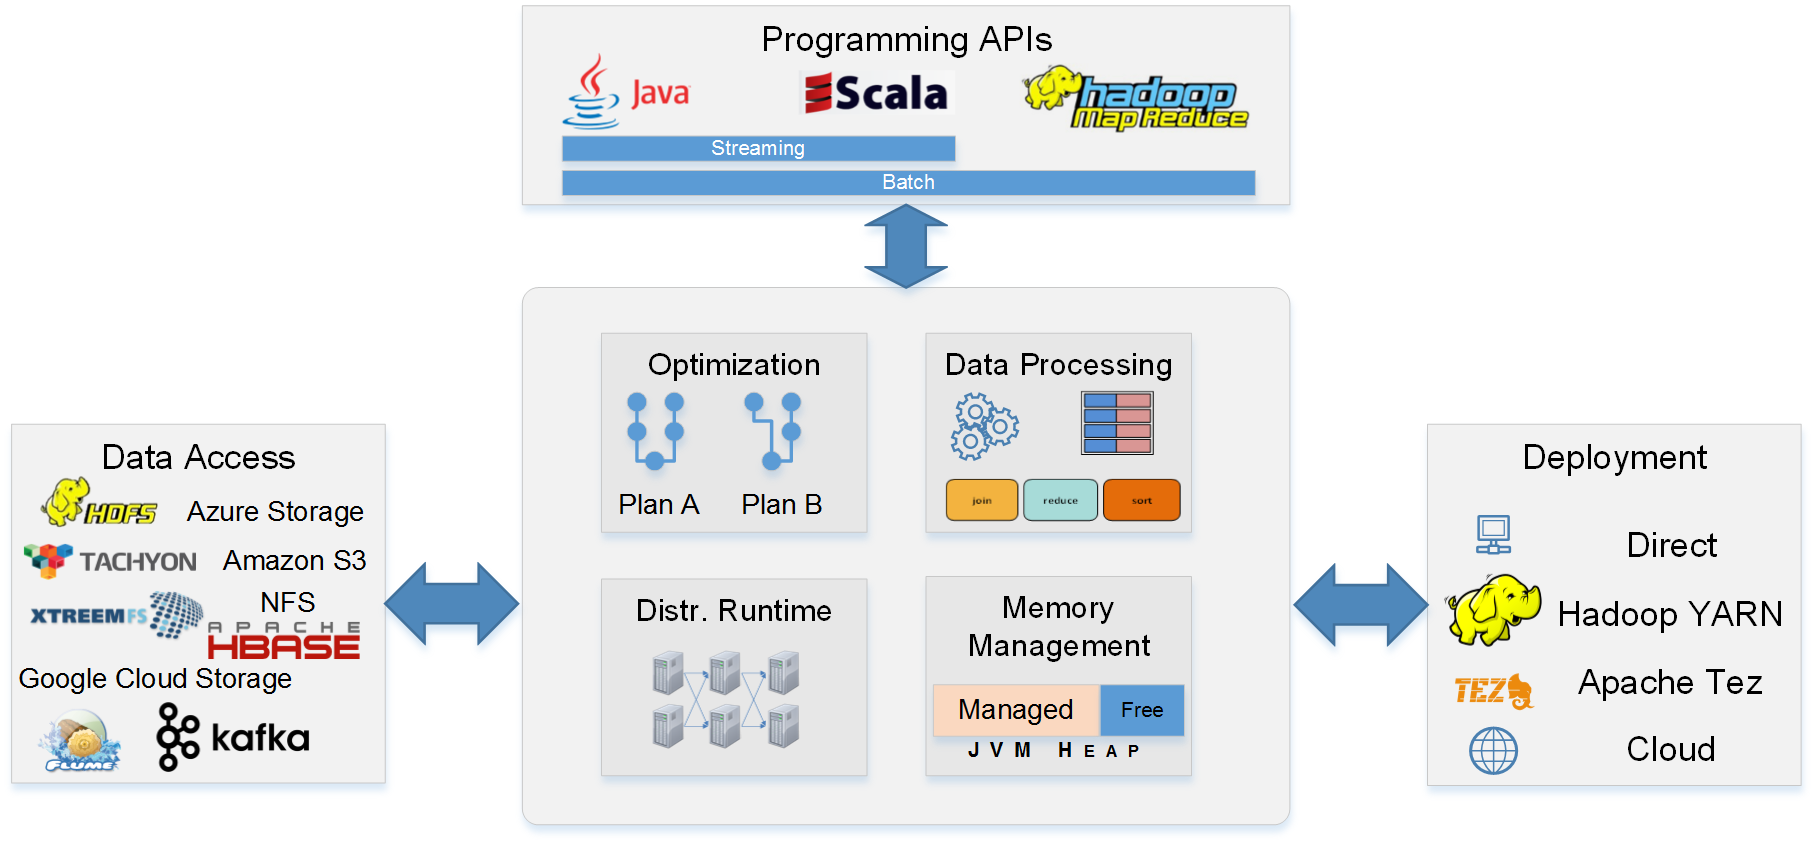
\includegraphics[width=1\textwidth]{ApacheFlink}
\caption{Apache Flink}
\label{fig:flink}
\end{figure}


Flink contains APIs in Java and Scala for analyzing data from batch and streaming data sources, as well as its own optimizer and distributed runtime with custom memory management (Figure~\ref{fig:flink})

However, similar to most of big data frameworks providing such rich APIs for imperative programing only, Flink is still struggling to gain traction from enterprise in relation of interaction UX.  First, users must spend time learning API documentation properly since those APIs are fairly new to them. Therefore, the cycle time to develop products taking longer. Second, given that most big data applications are fairly simple application-wise, a block of API codes might be less optimal to use for most the popular queries. We tackle solving the problem by building a extended version of ubiquitous SQL language on application layer of Flink. Since SQL is so popular, compact, well-design and easy to use, it is the most suitable choice to rely on for our extension. In the first step, this thesis aims to analyze and implement an SQL-extension (FlinkCQL - Flink Continuous Query Language) for Stream Processing Engine in Flink.

\subsection*{FlinkCQL and related works}
\textbf{//TODO}: missing

\subsection*{Structure}
We organize the thesis falls into 4 chapters:
\begin{itemize}
	\item Chapter 2: Data Stream Model in explains. The chapter describes the concept of data stream and what different between data stream and traditional database. 
	\item Chapter 3: The execution semantic dedicated to Flink Stream Processing. This part helps to understand how the streaming processing engine works under the hook.
	\item Chapter 4: FlinkCQL in details. We fully describe the specification of FlinkCQL syntax , as well as its semantics
	\item Chapater 5: Implementation of overall extensions.
\end{itemize}


\subsubsection*{My contribution:}
// TODO: add more information
\begin{itemize}
	\item Analyze the execution model of Flink Streaming
	\item Design and analyze language semantic of FlinkCQL
	\item Propose the architecture of implementation for FlinkCQL interpreter
\end{itemize}

%Challenge: so flexible on execution model : $t_{app}$ $t_{sys}$

%[2014] Fundamentals of Stream Processing- Application Design, Systems, and Analytics.pdf \citep{Henrique:2014}

%Sliding Window Query Processing over Data Stream  by Lukasz Golab




%Processing data streams is a a different paradigm, and moreover, Java is typicaly 50X less compact than say SQL – significantly more code required. Java and Scala require significant garbage collection which is particularly inefficient and troublesome for in-memory processing.
 
 
 
%\href {http://www.sqlstream.com/blog/2015/03/5-reasons-why-spark-streamings-batch-processing-of-data-streams-is-not-stream-processing/}{}

%BUILDING ALGEBRA SEMANTIC FOR FLINK STREAMING- IMPLEMENTATION

%*******************************************************************************
%****************************** Second Chapter *********************************
%*******************************************************************************

\chapter{Data Stream Model}

\ifpdf
    \graphicspath{{Chapter2/Figs/Raster/}{Chapter2/Figs/PDF/}{Chapter2/Figs/}}
\else
    \graphicspath{{Chapter2/Figs/Vector/}{Chapter2/Figs/}}
\fi


\subsection*{Order}
The concept of \textit{Order} is rather important in Distributed system, specially Stream Processing System in particular. 

In traditional model, there are a single program, one process, one memory space running on one CPU. Programs are written to be executed in an ordered fashion like a queue:  starting from the beginning, and then going towards the end. 

In distributed system, programs are designed to solve the same problems which one can solve on a single machine using multiple interconnected machines. Although these machines are physically located across the network with possible delays or failures, the system tries to reserve the order of the result as if running on a single machine only. In other words, the ideal is that a) we run the same operations and b) that we run them in the same order - even if there are multiple machines\citep{Mikito:2014}.

In theory, they have defined 2 types of orders: total order and partial order. 

\begin{defi}
 Paritial order \citep{Simovici:2008} is a binary relation $\leq$ over a set $P$ which is reflexive, anti-symmetric and transitive, i.e., which satisfies for all $a$, $b$ and $c$ in $S$:
 
 \begin{itemize}
	 \item $a \leq a$ (reflexivity)
	\item  if $a \leq b$ and $b \leq a$ then $a = b$ (antisymmetry) 
	\item if $a \leq b$ and $b \leq c$ then $a \leq c$  (transitivity)
\end{itemize}
\end{defi}

A set of elements, which is partially ordered, does not always ensure the order of  2 arbitrary elements. The natural state in a distributed system is partial order. Neither in the network nor between independent nodes the system is able to make any guarantee about relative order of two elements, probably due to many factors such as network latency, performance and so on; but at each node, one can observe a local total order.

\begin{defi}
 Total order \citep{Simovici:2008} is a binary relation `$\leq$' over a set $S$ which is anti-symmetric and transitive and total. Therefore, total order is a partial order with totality
 
 \begin{itemize}
	 \item $a \leq b$ or $b \leq a$  (totality)
\end{itemize}
\end{defi}

Total order ``<'' is strict on a set $S$ if and only if $(S, <)$ has no non-comparable pairs:
\begin{equation}
 \forall x, y \in S \Rightarrow  x < y \cup y < x 
\end{equation} 


In a totally ordered set, every two elements are comparable whereas in a partial ordered set, some pairs of elements are incomparable and hence we do not have the exact order of every element.

In streaming processing, one may not ask for entire stream  but rather a portion of data stream (i.e., window) periodically for further computation. For example, every 5 minutes, they would like to know the average volumes of last 100 transactions to detect any abnormal transaction. Any older element from $101^{th}$ will be discarded. Since the number of transactions is bounded within 100, the order of elements is crucially needed here to decide which one should fall into the window but others do not. This property also make stream processing model is different from rational data base system in which order of elements might not necessary. Traditional DBMS already knows the bounded data set involved in queries whereas stream processing engine has to decide its window based on the order.

Depend on the execution model of different systems, they may design different strategies of order such as temporal or positional order \citep{Petit:2012}.

The \textbf{temporal order} is induced by the timestamp of elements in a stream. Using the value of timestamp, one can determine whether something happen chronologically before something else. In practice, they usually use time as a source of order. System can attach timestamps to unordered events to maintain an order between events. Nevertheless, if some elements happen simultaneously, they will have the identical timestamp, then the order is total but non-strict. For instance, there are two elements with the same timestamps but system is required to take one element only, the chosen is non-deterministic between two because there is no difference between them in term of order. Therefore, we may require a strict order in order to avoid unfortunate random choices which mislead users about data stream's insight.

The \textbf{positional order} is a strict order induced by the position of elements in stream. Two elements  may have the same timestamp but one may arrive before the other so that they have different positional orders. The positional order can be defined by arrival order or id of element regardless of an explicit timestamp. 



\subsection*{Time}
\textbf{Time Domain} $\mathbb{T}$ is a discrete, total ordered, countably infinite set of time instants $t \in \mathbb{T}$. We assume that $\mathbb{T}$ is bounded in the past, but not necessarily in the future.

Time instant can be signified by either human-readable formatted string  such as ``Wed Aug 21 2013 00:00:00 GMT-0700 (PDT)'' or a \textit{Long} number as a milliseconds time value. In many high-level languages, the ``zero epoch'' moment $t = 0$ is usually set to the midnight of \textit{Jan 1 1970} and time unit is millisecond. Obviously, it is exchangeable between 2 representing formats.   
For the sake of simplicity, we will assume that the time domain is the domain of non-negative long number ($\mathbb{T} = \mathbb{N}$) {0,1,2,3,..} and totally ordered\citep{Dindar:2013}.

When considering the order, each event may be attached with either or both of : system time $t_{sys}$ (implicit) and application time $t_{app}$ (explicit). 

\textbf{Application Timestamps $t_{app}$}. In many case, each element in stream contains an explicit source-assigned timestamp itself. In other words, the timestamp attribute may be a part of the stream schema. To consider  a common log format for a web application which contains a timestamp specifying when the action is taken place. 
A log line records an action of user \textit{pablo} to get an image on Oct 10 2000:
\begin{verbatim}
216.58.209.174 user-identifier pablo [10/Oct/2000:13:55:36 -0700] 
"GET /image.gif HTTP/1.0" 200 1234
\end{verbatim}
Since web server may handle thousands of concurrent requests per second, it is possible to have many line of logs sharing a $t_{app}$ timestamp value. Therefore, application timestamp can be used as a source of total but non-strict ordering.

\textbf{System Timestamps $t_{sys}$}. Even if the element arrives at the system are not equipped with a timestamp, the system assigns a timestamp to each tuple, by default using the system’s local clock. While this process generates a raw stream with system timestamps that can be processed like a regular raw stream with application timestamps, one should be aware that application time and system time are not necessarily synchronized\citep{Kramer:2009}. Since system timestamp is assigned implicitly by system, one may not notice its presence on schema. 


Both application and system timestamp captures time information but they carry two different meanings. The former is related to the occurrence of the application event (when the event happens), whereas the latter is related to the occurrence of related system (when the corresponding event data arrive at system). Multiple elements may have the same application timestamps but they will not arrive in the same order. Therefore, system will assign the different unique system timestamp based on their arrival. System then can believe in the system timestamp as a strict total ordered basis for reasoning about arrival elements to perform processing. For example, another log from different users arrive at system:
\begin{verbatim}
219.53.210.143 user-identifier fabio [10/Oct/2000:13:55:36 -0700] 
"GET /image.gif HTTP/1.0" 200 1432
\end{verbatim}
However, it might arrive after the first log for user \textit{pablo} then system would response \textit{pablo}'s first, instead of \textit{fabio}'s request.

As we mentions above, in general, time domain is total ordered in local machine, but partial ordered across the system because of possible postpone on processing or asynchronous timestamp at different nodes. From now on, we are going to analyze the execution model of stream processing on logical layer which means that it work like it would on a single machine. Thus, we could assume that time domain is the source for total ordering.

%\textbf{\\TODO}: more on Timestamp in Streams \citep{Babcock:2002} page 13

\subsection*{Tuple}
A tuple is a finite sequence of atomic values. Each tuple can be defined by a \textit{Schema} corresponding to a composite type. Tuple can represent a relational tuple, a event or a record of sensor data and so on \citep{Arasu:2006}. For instance, the line of log in previous example follow a schema:

\begin{verbatim}
<SourceIP, IdentityType, user, timestamp, action, response, packageSize>
\end{verbatim}

A data tuple is the fundamental, or atomic data element, embedded in a data stream and processed by an application. A tuple is similar to a database row in that it has a set of named and typed attributes. Each instance of an attribute is associated with a value\citep{Henrique:2014}. Furthermore, one can consider a tuple as a partial order mapping a finite subset of attribute names to atomic values\citep{Petit:2012}. A tuple consists of a set of \textit{(Attribute $\times$ Value)} pairs such as $(SourceIP, 219.53.210.143)$


\section{Stream Model}


Based on time and tuple domain, basically, CQL in STREAM  \citep{Arasu:2006} engine defines a data stream as
\begin{defi}
	A stream $\mathbb{S}$ is a countably continuous and infinite set of elements $s:<v,t> \in \mathbb{S}$, where $v$ is a tuple belonging to the schema of $\mathbb{S}$ and $t \in \mathbb{T}$ is the timestamp of the element. 
\end{defi}

There are several definitions of data stream varying based on the execution model of systems. On the previous definition, a timestamp attribute can be a non-strict total ordered application timestamp so that system may not rely on it to select tuples on some operations requiring proper order between any pair of tuples. For this reason, stream can contain an extra physical identifier  $\varphi$ \citep{Petit:2010} such as increment tuple id to specify its order. The tuple with smaller id mean that they arrive and should be processed before the tuples with bigger id. Another way to identify the order of a tuple element is to separate the concept of application and system timestamp. In SECRET model \citep{Dindar:2013}, each stream element is composed of a tuple for event contents, an application timestamp, a system timestamp, and a batch-id value. The idea of batch-id is critical to SECRET system we do not mention in the thesis.
In short, we learn that elements of a stream are totally ordered by the system timestamp and physical identifier.

In Apache Flink, for the flexibility, system accepts a user-defined timestamp function   $f: \mathbb{TP} \rightarrow \mathbb{T}$ to map a tuple to its application timestamp value. One of the most common scenario is that the function $f$ extract one attribute of Schema and consider it as timestamp value in milliseconds.

Consider the example of temperature sensors, the sensors feed a stream $S(TIME\ :\ long,TEMP:\ int)$ indicating that at the moment of \textit{TIME}, the ambient temperature is \textit{TEMP}. Since $TIME$ attribute has the $long$ data type, we are able to consider it as a timestamp value due to function
\begin{equation}
f: (TIME, TEMP) \rightarrow TIME
\end{equation}

However, we may receive the stream signal from a different timezone. Thus, the application timestamp must be converted to the current timezone for the sake of data integration. For instance, one acquires the timestamp value (in milliseconds) in next timezone.
\begin{equation}
f: (TIME, TEMP) \rightarrow TIME + 3600*1000
\end{equation}


%%I propose the definition of Stream $s:<v>$ extends to $s:<v, t_{app}, t_{sys}>$, with $t_{app} = f(v)$, $t_{app} \in \mathbb{T}$, $t_{sys} \in \mathbb{T}$

For further analysis on execution model in Apache Flink, I propose a extend definition of a data stream as:
\begin{defi}
	A stream $\mathbb{S}$ is a countably infinite set of elements $s \in \mathbb{S}$. Each  stream element $s: <v, t_{app}, t_{sys}>$, consists of a relational tuple v conforming to a schema $S$, with an \textit{optional} application time value $t_{app} \in \mathbb{T}^*$ with $\mathbb{T}^* = \{-1\} \bigcup \mathbb{T}$ and a timestamp $t_{sys} \in \mathbb{T}^*$ generated automatically by system, due to the event arrival.
\end{defi}

With the partial function $f$ to extract an application timestamp value from tuple: $f: \mathbb{TP} \rightarrow \mathbb{T}$,
\begin{equation}
	t_{app} = 
	\begin{cases}
		f(v) \qquad\qquad if\,funtion\, f\, is\, defined\\
		   \\
		-1 \qquad\qquad\qquad otherwise
	\end{cases}
\end{equation}



 
\subsection*{Data Stream Properties} 
In the data stream model, some of all the input data that are to be operated are not available for random access from disk or memory, but rather arrive as one or more continuous data streams. 

%Data streams differ from the conventional stored relation model in several ways\citep{Babcock:2002}

Data Stream may have the following properties \citep{Golab:2010}:
\begin{itemize}
	\item They are considered as sequences of records, ordered by arrival time or by another ordered attributed such as generation time which is explicitly specified in schema, that arrive for processing over time instead of being available a priori. Totally order by time. 
	\item They are emitted by a variety of external sources. Therefore, the system has no control over the arrival order or data rate, either within a stream or across multiple streams
	\item They are produced continually and, therefore, have unbounded, or at least unknown, length. Thus, a DSMS may not know if or when the stream ``ends''. We may set a time-out waiting for new event. Exceeding the time-out, the stream considerably terminated. 
	\item Typically, big volume of data arrives at very high speed so that data need to process on the fly. Once an element from a data stream model has been processed it is discarded or archived. Stream elements cannot be retrieved, unless it is explicitly stored in storage or memory, which typically is small relative to the size of the data stream\citep{Babcock:2002}.
	
\end{itemize}


\subsection*{Stream Representations}
\subsubsection*{Base Stream vs. Derived Stream}
We distinguish 2 kinds of streams: \textit{base stream}(source stream) and \textit{derived stream}. Base stream stream is produced by the sources whereas derived stream is produced by continuous queries and their operators\citep{Arasu:2006}. 
%For example, \citep{Golab:2010} page 17
From now on, we give example queries on input stream named \textit{StockTick}\citep{StreamBaseTut} and the schema associated with the incoming tuples includes 4 fields:
\begin{itemize}
\item \textbf{Symbol}, a string field of maximum length 25 characters that contains the symbol for a stock being traded (e.g. IBM);
\item \textbf{SourceTimestamp}, a timestamp field containing the time at which the tuple was generated by the source application(timestamp is represented with date time format or long integer);
\item \textbf{Price}, a double field containing transaction price
\item \textbf{Quantity}, a integer fields that contains the transaction volume
\item \textbf{Exchange}, a string field of maximum length 4 that contains the name of Exchange the trade occurred on (e.g. NYSE)

\end{itemize}
A sample tuple represents the price of IBM stock unit is 81.37 at ``1 May 2015 10:18:23" from NYSE market 
\begin{verbatim}
<IBM,1430468303,81.37,NYSE>
\end{verbatim}

The \textit{StockTick} is emitted directly from source so that it is a base stream. However, a below \textit{HighStockTick} stream is a derived stream originated from \textit{StockTick}. \textit{HighStockTick} contains only transaction of stock with price of more than \$100 each unit.

\begin{verbatim}
CREATE STREAM HighStockTick AS
	SELECT * FROM StockTick 
	WHERE price > 100
\end{verbatim}

In practice, base stream are almost always append-only, mean that previously arrived stream elements are never modified. However, derived stream may or may not be append-only\cite{Golab:2010}. A derived stream that present the average transaction volumes between interval time $[t_1, t_2]$. The query produce an element $s_1$ to the stream immediately after $t_2$. However, an element of \textit{StockTick} stream with timestamp 
$t_{12} \in [t_1,t_2]$ arrive late at $t_2+\phi$. If the system takes into account of the late arrival element, it will update the previous average volumes at $[t_1, t_2]$. In this case, this derived stream is not append-only. Unfortunately, Flink has not supported Delay function, so that all stream is apparently append-only.


%\textbf{Note}: another examples from \textbf{epl-guide}
%\textbf{Note}: stock example : http://www.codeproject.com/Articles/553206/An-Introduction-to-Real-Time-Stock-Market-Data-Pro


\subsubsection*{Logical Stream vs. Physical Stream}
%// TODO : Logical vs. physical stream ?  \citep{Kramer:2009}

Logical stream is a conceptual and abstract data stream which is processed linearly through a series of chaining operators. According to logical data flow graph, one is able to observe the order of operators that data is processed and what are the input and output of process.

Physical stream flow graph indicates how system really process the data in data parallelism environment. Physical operator is replicated and the internal operator state is partitioned and segmented. Figure~\ref{fig:streamRepresent} depicts the different between logical and physical data flow.
A logical stream from source go straight through an aggregate and a filter operator before written to Sink, whereas physical streams are segmented and go through different internal replica of the same logical operator. Eventually, all physical streams will be merged and written to one Sink. 

%\begin{wrapfigure}{l}{0.7\textwidth} 
 %   \centering
  %  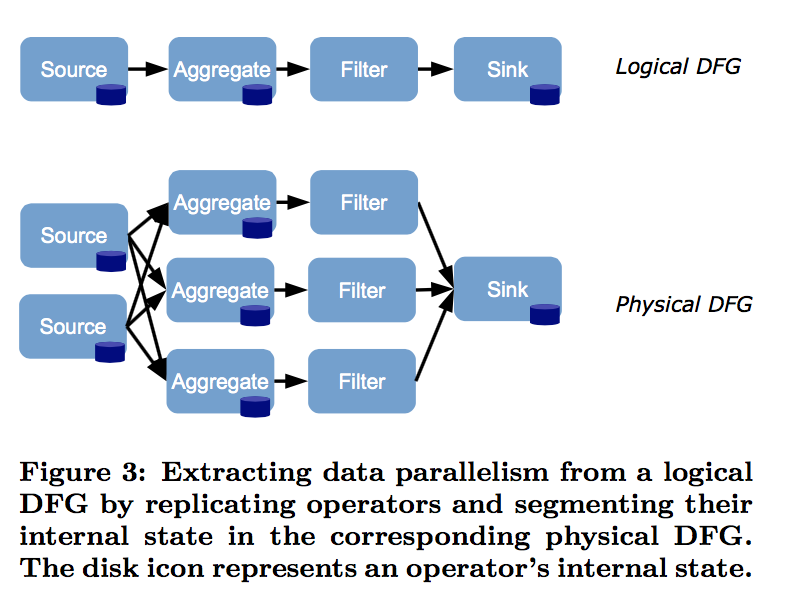
\includegraphics[width=0.7\textwidth]{logicalPhysicalDataFlow}
%\caption[Minion]{Stream Processing in Action. Henrique Andrade}
%\label{fig:streamRepresent}
%\end{wrapfigure}

\begin{figure}[htbp!] 
\centering    
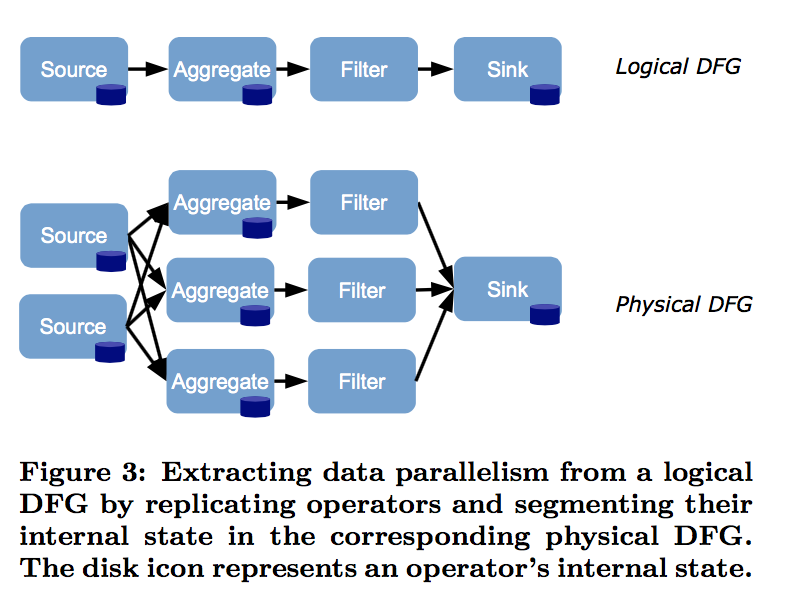
\includegraphics[width=0.7\textwidth]{logicalPhysicalDataFlow}
\caption[Minion]{Extract data parallelism from a logical DFG by replicating operators and segmenting their internal state in the corresponding physical DFG. The disk icon represent an operator's internal state \citep{Henrique:2013}}
\label{fig:streamRepresent}
\end{figure}

   
%\subsection*{Signals[Option] \citep{Golab:2010}}     
    
    
\section{Stream Windows}

From the system's point of view, it is often infeasible to maintain the entire history of the input data stream. Because data stream is running infinitely, we may not know exactly when it ends. It nearly impossible to query over the entire stream with some operators such as sum, average. Accumulating a tuple attribute for entire stream may results to a very big value causing  buffer overflow.  When a bounded amount of memory is limited, hence it is barely capable of producing exact answers for data stream queries. Nevertheless, high-quality approximate answers are often acceptable instead. 

We have seen many techniques to tackle the problem such as sketches, random sampling, histogram and so on. However, the most preferred technique is windowing technique which continually runs queries over recent portion of data stream  in lieu of then entire of its past history. For examples, every 10 minutes, asking for total numbers of transaction happened last hour only. The semantic of window is clear and well-defined that makes it easy to operated by system and understood by users. The size of window is relatively smaller than size of stream so that system can keep latency of computation low.  More importantly, from the user's point of view, recent data may be more insightful and informative to make a data-driven decision immediately. Those reasons motivated the use of windows to restrict to the scope of continuous queries. Indeed, many stateful stream processing operators are designed to work on windows of tuples, making it a fundamental concept in stream processing. Therefore, a stream processing language must have rich windowing semantics to support the large diversity in how stream processing engine can consume data on a continuous basis.


\begin{defi}
A \textbf{Window} $W$ over a stream $\mathbb{S}$ is a finite subset of stream $\mathbb{S}$ \cite{Dindar:2013}
\end{defi}


A window over streaming data can be created, buffering a continuous sequence of individual tuples. However, the size of window is a finite number so that system must decide what and how to buffer data based on the window specification. 

The specification consists of several parameters :
\begin{enumerate}
\item an optional partitioning clause, which partitions data in window into several groups. Query on window will be taken place regard for each group, instead of the whole window
\item a window size, that may be expressed either as the number of tuples included in it or as the temporal interval spanning its contents
\item an window slide, the distance between the starts of 2 consecutive window (i.e., waiting 2 seconds or 5 data elements before starting a new window). This crucial property determine whether and in what way a window change state over time. If the window slide parameter is missing, system can  assign implicitly that the slide size is equal to the window size. In this case, we have a stream of disjoint windows so called batch windows or tumbling windows.
\item an optional filtering predicate, keeping only elements that satisfy the predicate.
\end{enumerate}

For example, a window specification 
\begin{lstlisting}
	[
		SIZE 3 hours EVERY 1 hours 
	 	PARTITIONED BY Exchange
	 	WHERE Quantity > 100.000
	 ]
\end{lstlisting}
means that window cover all transactions with $Quantity > 100.000$ over last 3 hours once every 1 hour. Transaction tuples inside the window are partitioned into groups specified by Exchange keyword Figure~\ref{fig:winSpec}
\begin{lstlisting}
	[
		SIZE 3 hours EVERY 1 hours 
	 	PARTITIONED BY Exchange
	 	WHERE Quantity > 100.000
	 ]
\end{lstlisting}

\begin{figure}[htbp!] 
\centering    
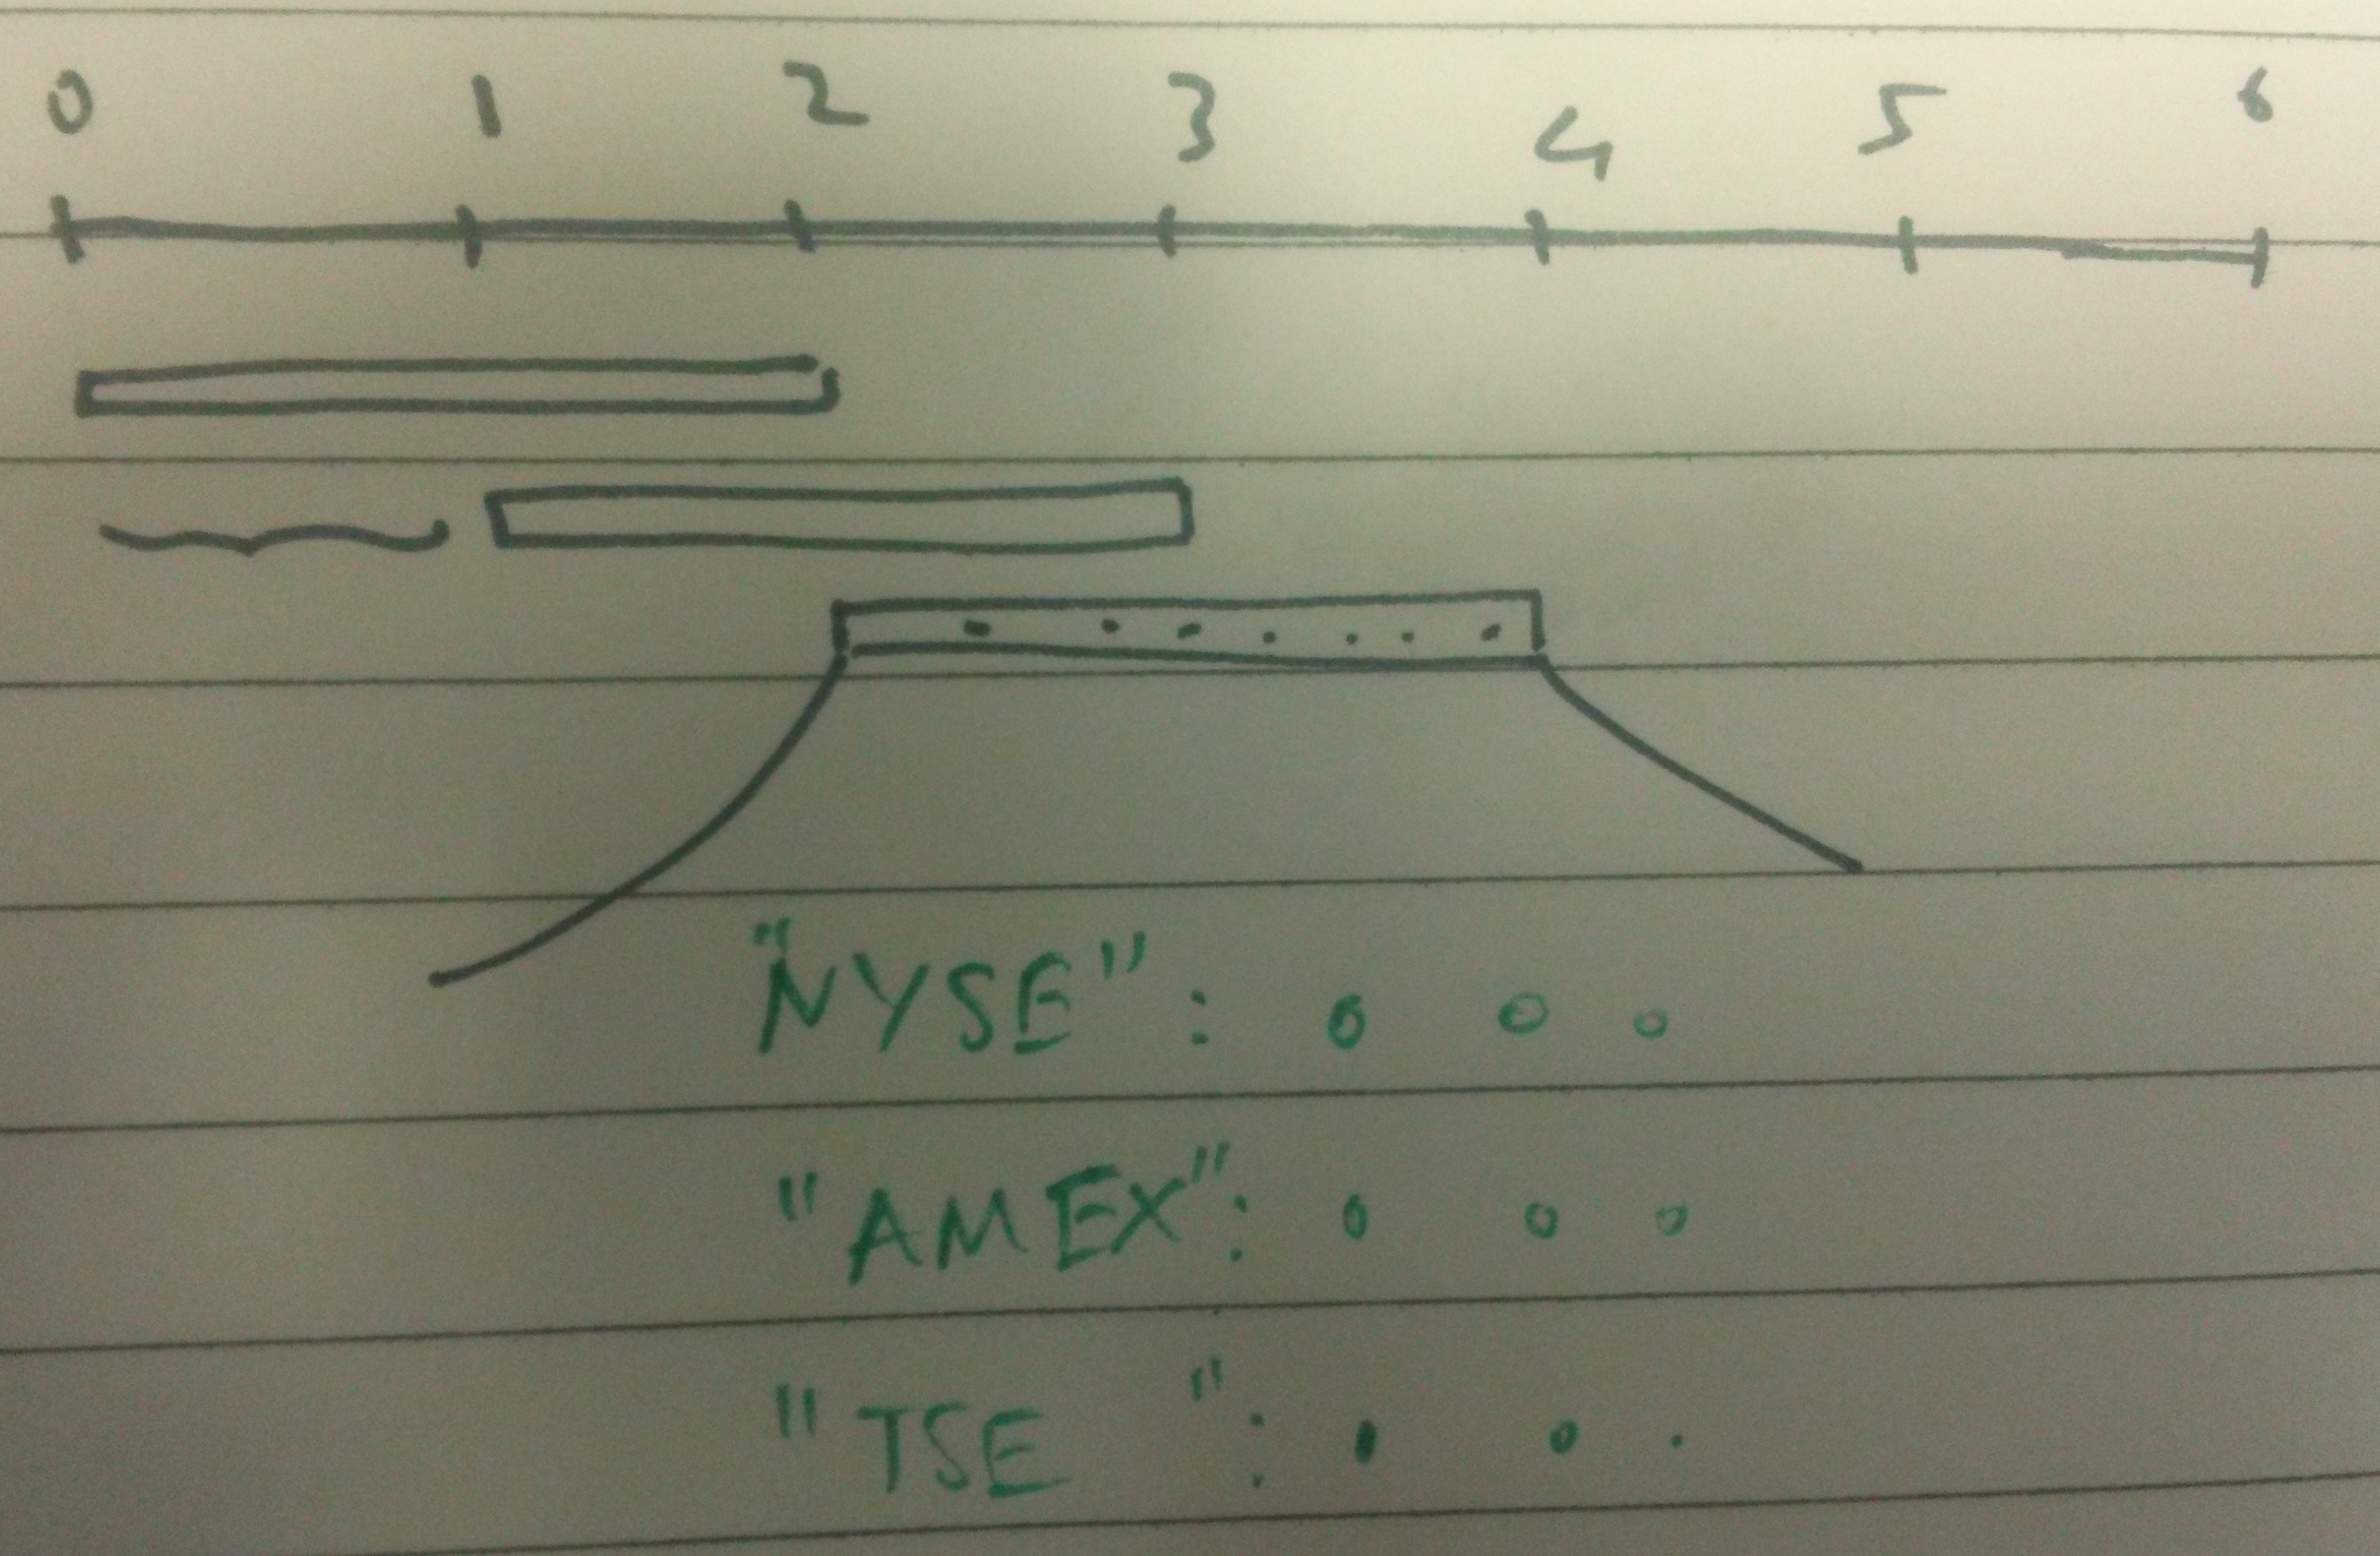
\includegraphics[width=0.7\textwidth]{winSpec}
\caption{Windowed Stream}
\label{fig:winSpec}
\end{figure}

Windows can be construct according to (window specification) that defines what to buffer, resulting in many window variations. These variations differ in their policies with respect to evicting old data that should no longer be buffered, as well as in when to process the data that is already in the window.\citep{Henrique:2014}


Window may be classified according the following criteria:

\subsection{Direction of movements}
Window can fixed or sliding along the stream.
\begin{itemize}

\item Fixed Window:  has both upper-bound and lower-bound fixed. Therefore the window is evaluated only once and capture a constant portion information of stream. For instance, window stores the transactions generated in 2 hours from ''2015/01/01 12:00:00" to ''2015/01/01 14:00:00"

\item Landmark Window: One of the bounds remains  anchored at a specific system timestamp. The other edge of the window is allowed to move freely. Usually, the lower-bound is fixed, and the upper-bound shifted forward in pace with time progression.
For example, windows capture all transaction from 1a.m once every hour. Figure~\ref{fig:landMarkWin}

\begin{figure}[htbp!] 
\centering    
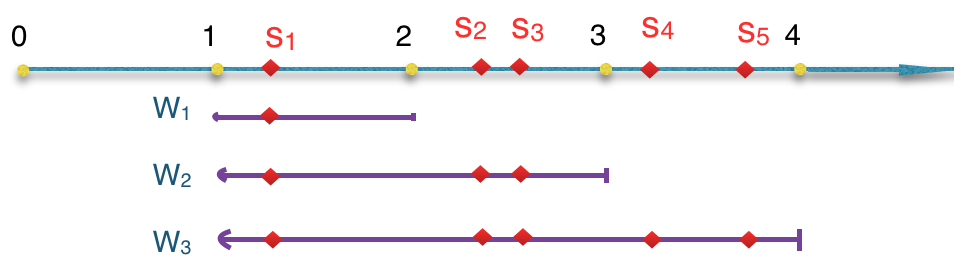
\includegraphics[width=0.7\textwidth]{landMarkWin}
\caption{Landmark Window}
\label{fig:landMarkWin}
\end{figure}

Up to 4am, the stream contains 3 window 
\begin{itemize}
\item $W_1(1,2):\{s_1\}$ 
\item $W_2(1,3):{s_1, s_2, s_3}$ 
\item $W_3(1,4):{s_1, s_2, s_3, s_4,s_5}$ 
\end{itemize}

\item Sliding window: the width of the window may be fixed in term of logical unit (i.e., time interval units) or physical unit (i.e., tuple count in window). However, the boundaries of windows change overtime along the stream.

For example, window contains last 3 transactions once every 1 transaction passed. Up to 4am, the stream contains 5 windows. Figure~\ref{fig:slideWin}
\begin{itemize}
\item $W_1:\{s_1\}$ : at the beginning there is only tuple $s_1$ on stream
\item $W_2:{s_1, s_2}$ there are only tuple $s_1$ and $s_2$ on stream. Window may take up to 3 tuples so that both $s_1$ and $s_2$ are included  
\item $W_3:{s_1, s_2, s_3}$ 
\item $W_4:{s_2, s_3, s_4}$ there are 4 tuples on stream but window can take last 3 tuples only. Therefore, window buffer will insert $s_4$ and drop $s_1$
\item $W_5:{s_3, s_4,s_5}$  window buffer insert $s_5$ and drop $s_2$
\end{itemize}

\begin{figure}[htbp!] 
\centering    
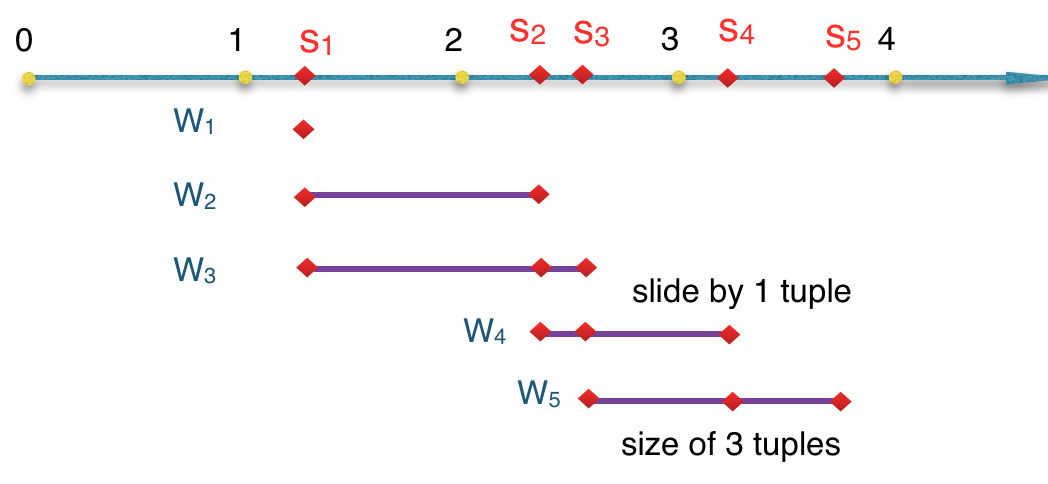
\includegraphics[width=0.7\textwidth]{slideWin}
\caption{Sliding Window}
\label{fig:slideWin}
\end{figure}



\item Tumbling window: a particular sliding window where the boundaries move is equal to the window's width. Windows are disjoint or non-overlapped each other. Windowed stream will cover all elements on based stream.

Example: For example, window contains last 2 transactions once every 2 transaction passed. Up to 5am, the stream contains 3 windows. Figure~\ref{fig:tumblingWin}

\begin{itemize}
\item $W_1:\{s_1,s_2\}$ 
\item $W_2:\{s_3, s_4\}$ 
\item $W_3:\{s_5,s_6\}$ 
\end{itemize}

\begin{figure}[htbp!] 
\centering    
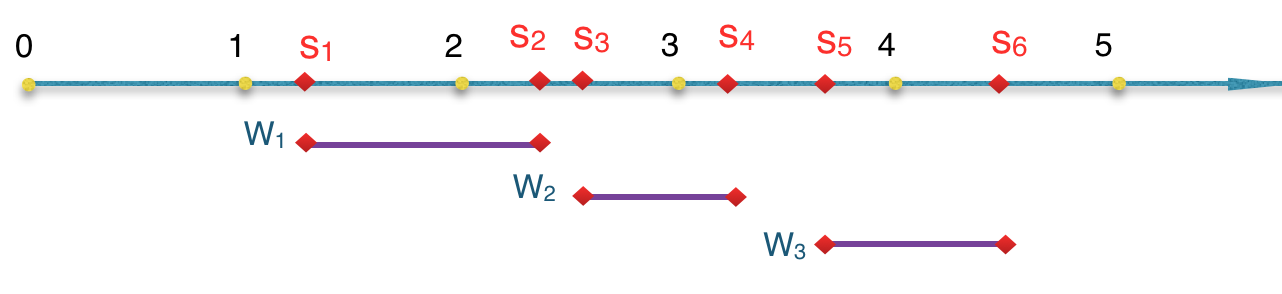
\includegraphics[width=0.8\textwidth]{tumblingWin}
\caption{Tumbling Window}
\label{fig:tumblingWin}
\end{figure}


\item Jumping window: a particular sliding window where the boundaries move is larger than the window's width. Windows are disjoint or non-overlapped each other but some of tuples may be discarded. For example, window contains last 2 transactions once every 4 transaction passed. Up to 5am, the stream contains 2 windows. Figure~\ref{fig:jumpingWin}
\begin{itemize}
\item $W_1:\{s_3,s_4\}$ When $s_4$ has arrived, window buffer contains 4 tuples $\{s_1,s_2,s_3,s_4\}$ but window's width is 2 so that $\{s_1,s_2\}$ will be evicted from window. Window buffer keeps $\{s_3,s_4\}$ then emits $W_1$
\item $W_2:\{s_7, s_8\}$ Window buffer evicts $\{s_5,s_6\}$, keeps $\{s_7,s_8\}$ then emits $W_2$
\end{itemize}

\begin{figure}[htbp!] 
\centering    
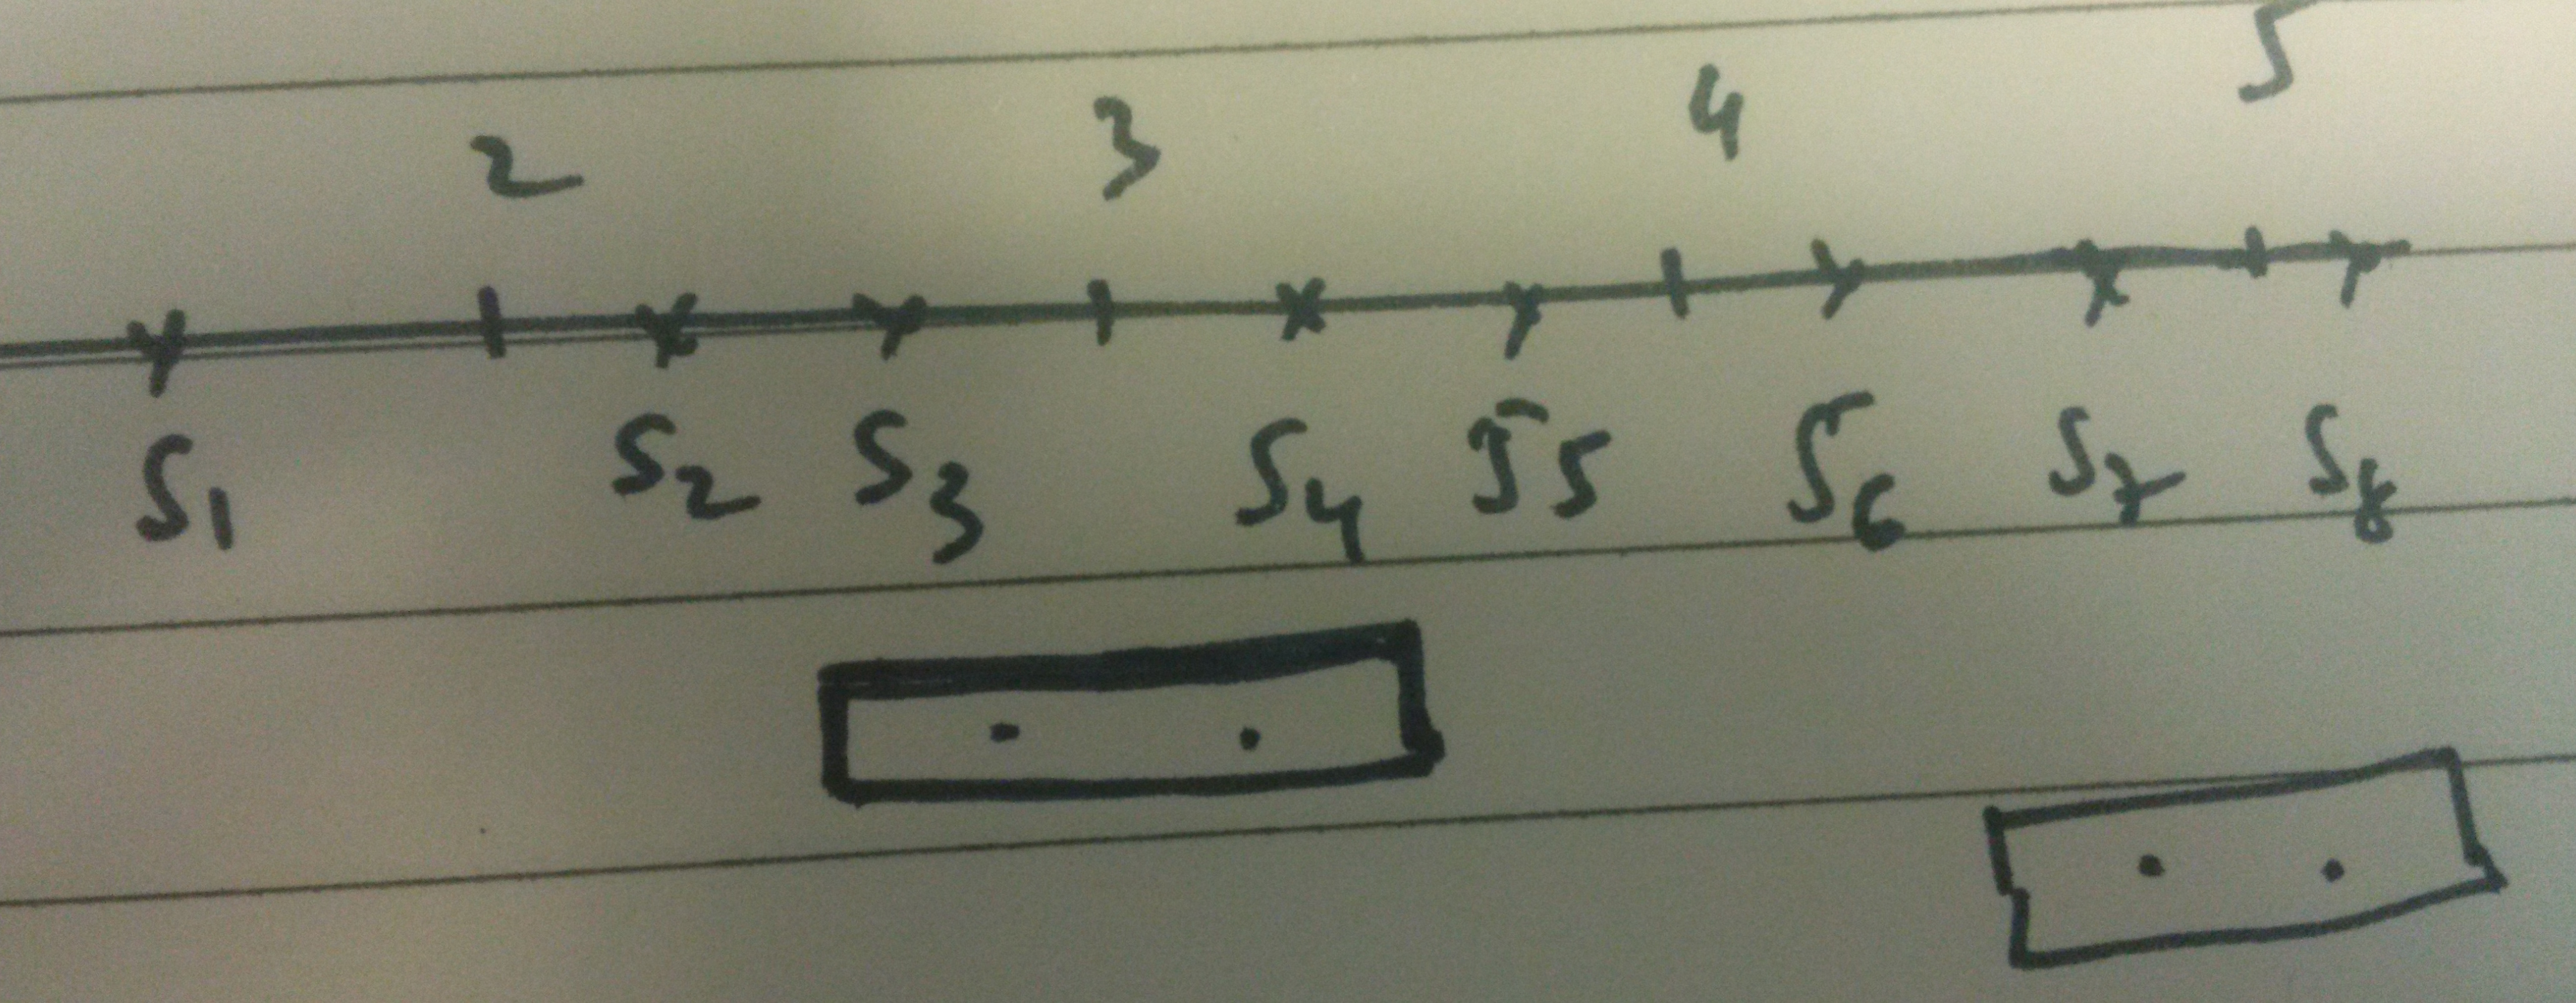
\includegraphics[width=1\textwidth]{jumpingWin}
\caption{Jumping Window}
\label{fig:jumpingWin}
\end{figure}


\end{itemize}


\subsection{Definition of contents} 

\begin{itemize}
	\item Logical or time-based windows are defined in terms of time interval, e.g., a time-base sliding window may maintain the the last one minutes of data.
	
	\item Physical(also known as count-based or tuple-based) windows are defined in terms of the number of tuples, e.g., a count-based window may store the last arrived 100 tuples.
	
	\item Delta-based windows are defined in terms of a delta function and a threshold value. The function calculates a delta between 2 elements such as absolute distance or Euclidean distance between 2 data elements. In delta-based windows, the delta between the first element and any of the rest must not be larger than the threshold, respectively. Currently new arrival data point will join the window if the delta between it and the first elements of window is equal or less than threshold. Otherwise, the window is closed and emitted; the currently arrival data point trigger a new window. 
	
Formally, a delta windows $W$ contains $n$ interval ordered elements $s_1, s_2,...,s_n$ continuously so that every elements $a_k$ with $k \in [1,n]$ must satisfies
	\begin{equation}
		\Delta(s_1,s_k) \leq \phi
	\end{equation}

There is a new arrival tuple $s_{n+1}$.
\begin{itemize}
\item if $\Delta(s_1,s_{n+1}) \leq \phi$, $s_{n+1}$ will join window $W$
\item Otherwise, window $W$ is closed and emitted for further computation. $s_{n+1}$ will trigger new window $W': \{s_{n+1}\}$
\end{itemize}

	
For example, assuming that stream $S$ contains 4 tuples so far (Figure~\ref{fig:deltaWin}). Element in window $W$ must satisfy the condition that the absolute distance between it and the first elements is not higher than 10.

Up to the moment $s_4$ has processed, Stream $S$ is discretized into window streams of 
\begin{itemize}
\item $W_1:\{s_1,s_2, s_3\}$ satisfies $\Delta(s_k,s_1) =|s_k-s_1| < 10 $ where $k \in [1,3]$
\item $W_2:\{s_4\}$ because $\Delta(s_4,s_1) = |s_4-s_1| = 12 > 10$, $s_4$ trigger a new window $W_2$
\end{itemize}

\begin{figure}[htbp!] 
\centering    
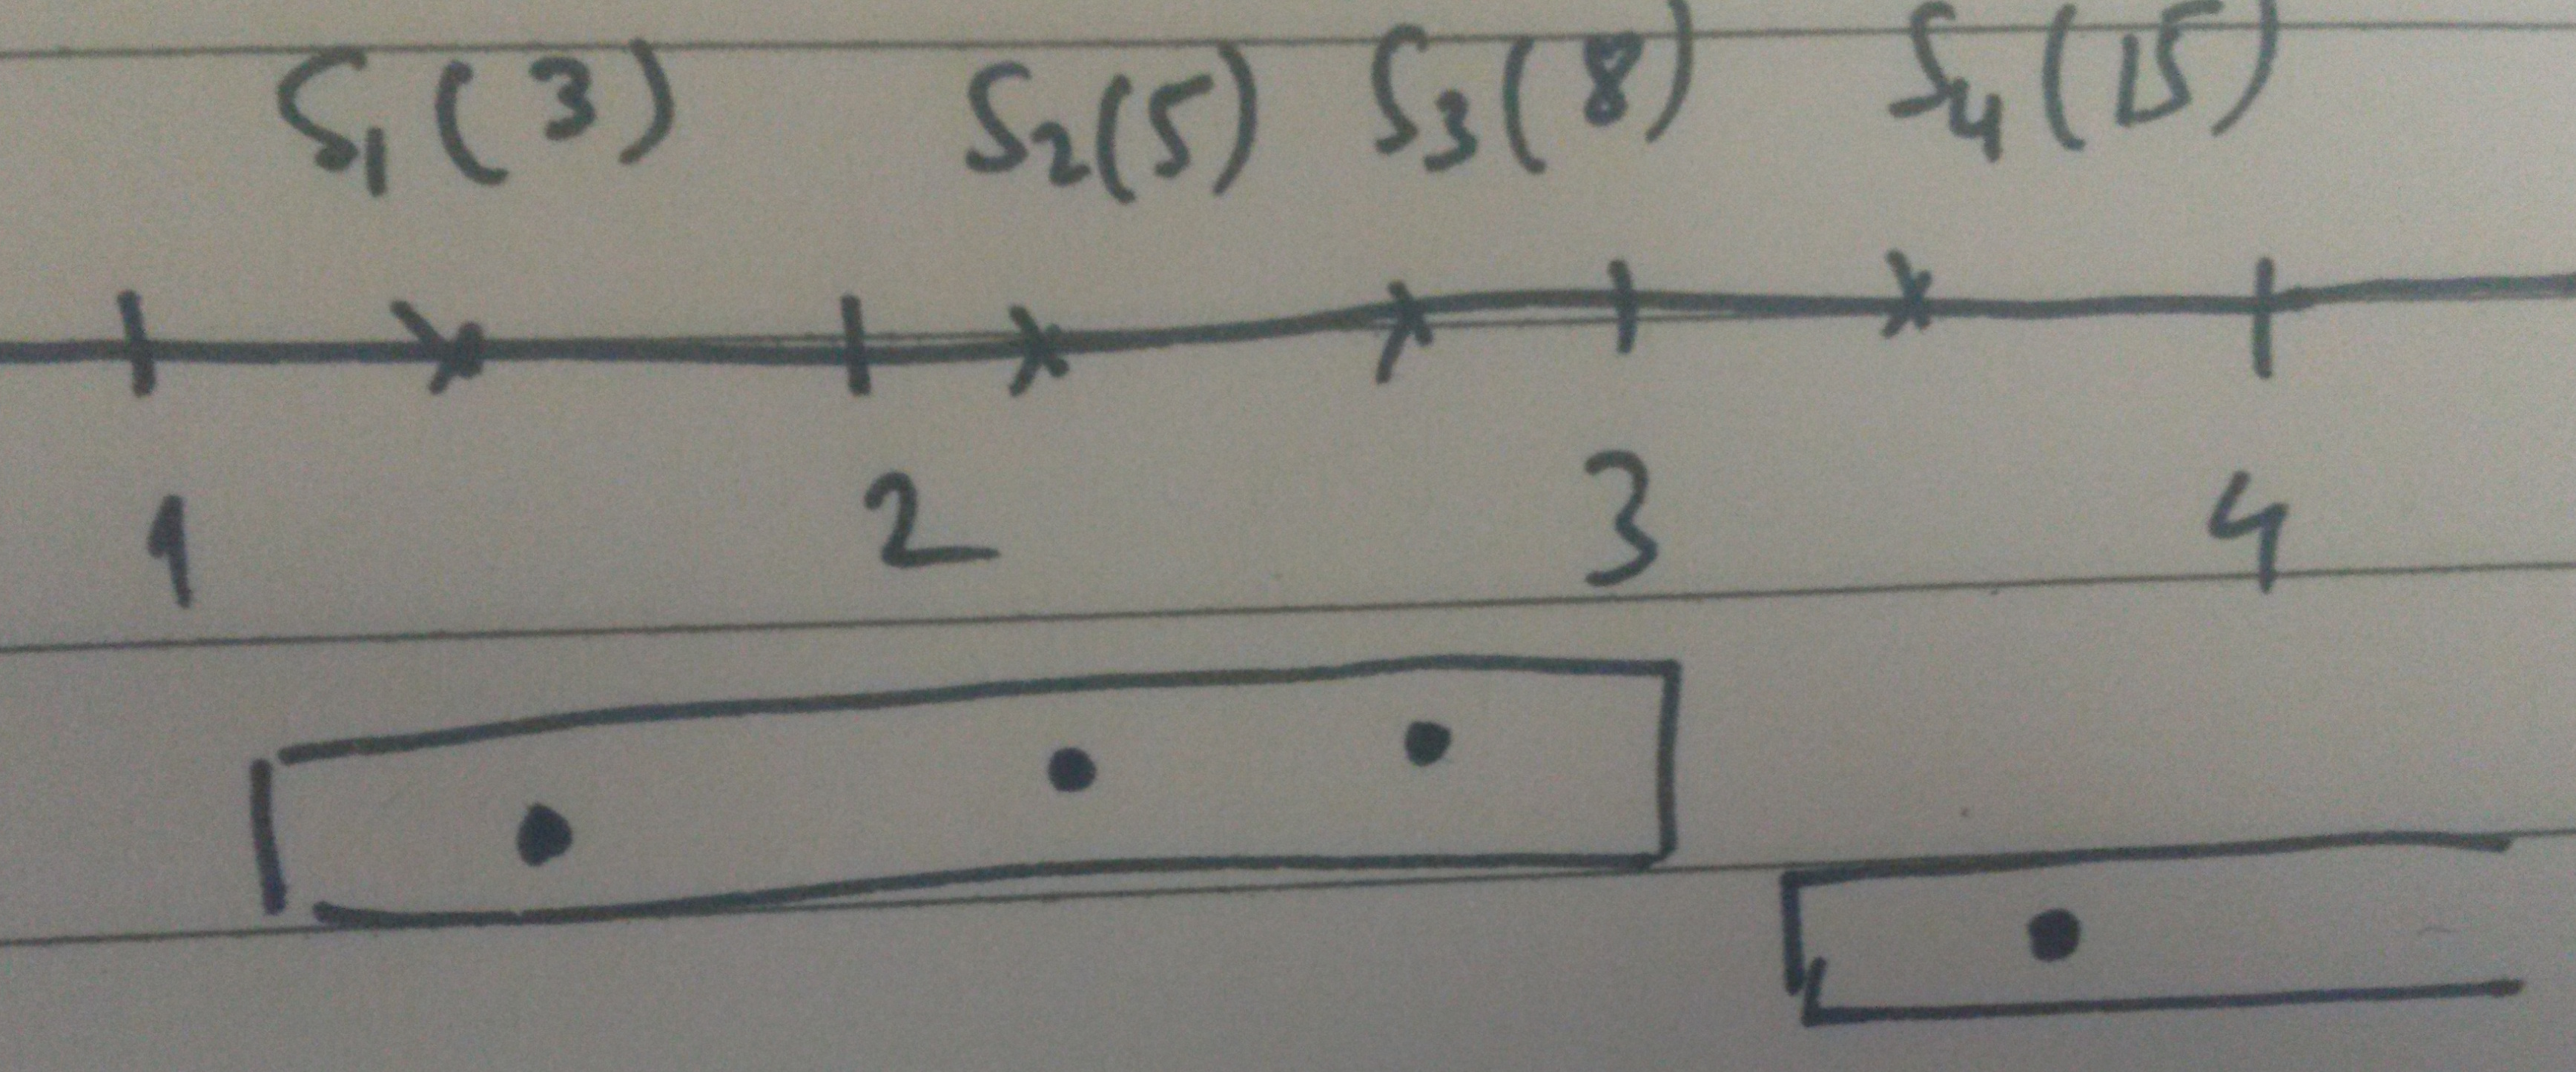
\includegraphics[width=1\textwidth]{deltaWin}
\caption{Delta-based Window}
\label{fig:deltaWin}
\end{figure}



	\item Partitioned Windows contain only the elements  in the same group which differentiates itself from the other groups  by the value of a grouping attributes (subset of its schema), e.g., a partitioned window store last 100 elements with the same value of (\textit{StockSymbol}, \textit{Exchange})(Figure~\ref{fig:partitionedWin}). Thus, several  substreams are derived logically from the base stream, each one is represented by an existing combinations of value$<a_1,a_2,...,a_k> \in Dom(S)$ on the grouping attributes $<A_1, A_2,...,A_k> \subset S$ ($S$ is schema of tuples, $Dom(S)$ is domain of $S$). Each group maintains a separate window buffer to capture arrival events and emit when satisfies window specification.
	
\begin{figure}[htbp!] 
\centering    
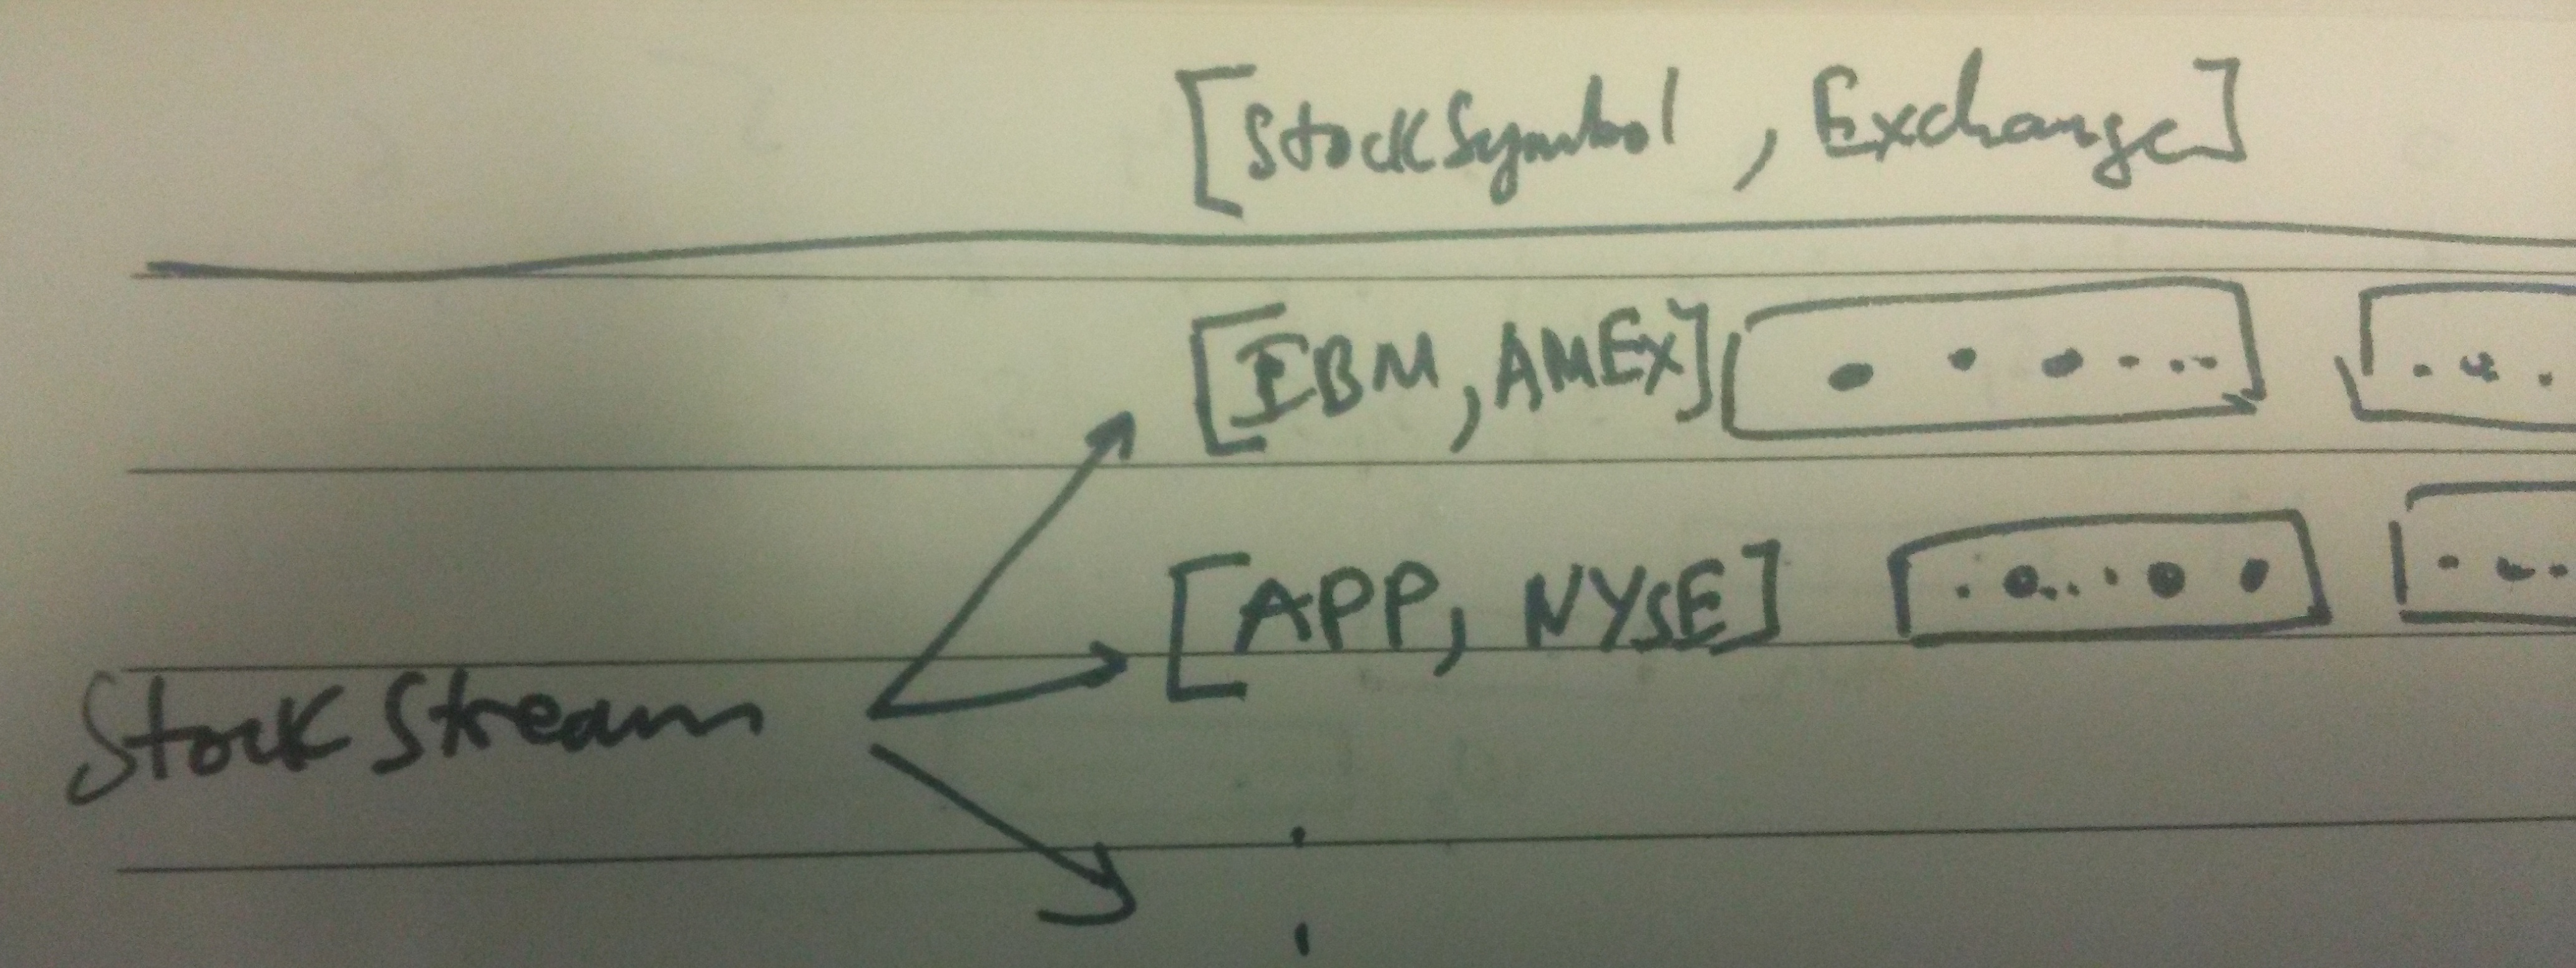
\includegraphics[width=0.75\textwidth]{partitionedWin}
\caption{Partitioned Window}
\label{fig:partitionedWin}
\end{figure}
	
%	\textbf{TODO: check Towards a Streaming SQL standard page 1385}
	
	
	
	\item Predicate window \citep{Ghanem:2008}, in which an arbitrary logical predicate specifies the contents. Only tuples that satisfies the predicate will join the window, otherwise it is discarded. e.g.,predicate window maintain last 100 transactions which have more than 100.000 units in terms of \textit{volume}, respectively. Every transaction with fewer quantity will be discarded.
	
\end{itemize}

%\subsection{Frequency of movement[Optional]} jumping window, mixed jumping window, tumbling window

%By default, a time-based window is updated at every time tick, and a count-based window is updated when a new tuple arrives. A jumping window is updated every k ticks or after every kth arrival. Note that a count-based window may be updated periodically, and a time-based window may be updated after some number of new tuples have arrived; these are referred to as mixed jumping windows [Ma et al., 2005]. If k is equal to the window size, then the result is a series of non-overlapping tumbling windows [Abadi et al., 2003].
%In practice, tumbling windows, such as the one-minute windows in query Q1 from Sec- tion 2.1.1, are popular due to the simplicity of their implementation—at the end of each window, the query resets its state and starts over. Forward-sliding windows (time-based and count-based) are also appealing due to their intuitive semantics, especially with joins and aggregation, as we will discuss below. However, sliding windows are more difficult to implement than tumbling windows; over time, a continuous query must insert new tuples into a window and remove expired tuples that have fallen out of the window range.


%\textbf{//TODO}:(check Sliding Window Query Processing over Data Stream pages 25)


%The notion of sliding windows requires at least an ordering on data stream elements. In many cases, the arrival orders of the elements suffices as an \"implicit timestamp\" attached to each data element. However, sometimes it is preferable to user \"explicit timestamp\" provided as part of data stream. Formally, we say that a data stream consists of a set of (tuple, timestamp) pairs. Timestamp attribute could be a traditional timestamp or it could be a sequence number - all that is required is that it come from a totally ordered domain with a distance metric. The ordering induced by the timestamp is used when selecting the data elements making up a sliding window. 


%\textbf{Notes}: in CQL tuple-based sliding window may be non-deterministic - and therefore may not be appropriate - when timestamp are not unique


%\textbf{Notes}: Tuple relational calculus by Edgar F. Codd

%\textbf{Notes}: \href{http://en.wikipedia.org/wiki/Relational\_algebra}{http://en.wikipedia.org/wiki/Relational\_algebra}


%*******************************************************************************
%****************************** Second Chapter *********************************
%*******************************************************************************

\chapter{The execution semantic of Stream Processing in Flink (10 pages)}

\ifpdf
    \graphicspath{{Chapter3/Figs/Raster/}{Chapter3/Figs/PDF/}{Chapter3/Figs/}}
\else
    \graphicspath{{Chapter3/Figs/Vector/}{Chapter3/Figs/}}
\fi

\section{Heterogeneity}\label{Heterogeneity}
Since the first commercial project of Complex Event Processing launched by Bell Labs in 1998 with its "Sunrise Project", we have seen the fast growing of many stream processing frameworks. However, there is a huge degree of heterogeneity across these frameworks in various forms\citep{Dindar:2013}

\begin{enumerate}

	\item Syntax: Although the ISO/IEC 9075 is published standard to defines the complete syntax and operations in SQL language as a whole, there is no standard language for stream processing. Different stream processing engines use different syntax to depict the same function. For example,every 5 seconds, a window captures all event last 10 seconds. 
	\begin{verbatim}
	CQL: 	[RANGE 10 seconds SLIDE 5 second ] 
	Flink: 	[SIZE 10 sec EVERY 5 sec]
	\end{verbatim}
	
	\item Capability heterogeneity:
	Those engines also provide different set of query types and operations based on which functions they are capable of. For examples, \textit{Streambase} support pattern matching on stream, whereas STREAM does not.
	
	\item Execution Model: Below the language level, hidden from application layers, each stream processing engine has its own underlying execution model. With the same data stream but different model produce different output which varies based on the differences on tuple ordering,  window construction, evaluation and so on. We are going to focus on the differences between several existing execution models below.
	
	
\end{enumerate}
 
We have learned that there are at least three different execution models:
\begin{itemize}
	\item \textbf{Time-driven} execution model, followed by CQL, Oracle CEP. In the model, each tuple have a timestamp. Timestamp induces the total order of tuples on stream, but not a strict total order. Or more specifically, there is no ordering between tuples with identical timestamps. These tuples are consider as simultaneous tuples. It is problematic when we select a window of last 10 tuples but more than 10 simultaneous tuples arrived at a given time instant. In this case, there is no different between those tuples, the system will select only 10 out of all in a non-deterministic way.
	
Assuming that we has stream $\mathbb{S}$
	\begin{equation}
			\mathbb{S}(value, t_{app}) = (1,1),(10,2),(20,2), (100,3)
	\end{equation}
	

	
Consider a query which continuously recall the last arrival tuple i.e., we select tuple-based window with size of 1 tuple. In the time-based execution model,  the state of a window changes as timestamp progress. Window get re-evaluated only when timestamp change. At $t=1$ or $t=3$, there is only 1 arrival tuple, new 1-tuple-size window will open , pick the tuple then close. Thus the stream derives window $W_1: \{(1,1)\}$ and $W_3: \{(100,3)\}$. On other hand, at $t=2$, there are 3 new arrival tuples. New window $W_2$ opens and be able to pick 1 tuple only. Since these 3 tuples arrive simultaneously, they will have the same timestamp and thus no any temporal differences between them.
Engine randomly pick one of them for window $W_2$. In short, window $W_2$ contains one of following options: $(10,2)$ or $(20,2)$. The derived stream will be one of the streams:
\begin{verbatim}
(1,1),(10,2), (100,3) or (1,1),(20,2), (100,3)
\end{verbatim}

\begin{figure}[htbp!] 
\centering    
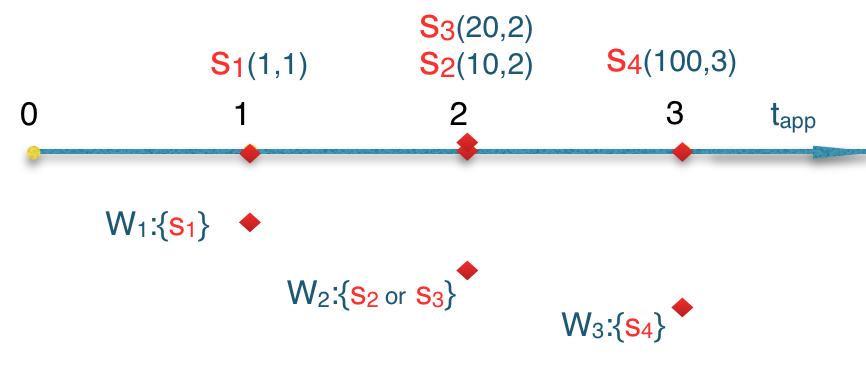
\includegraphics[width=0.5\textwidth]{time-driven}
\caption{time-driven}
\label{fig:time-driven}
\end{figure}
	
	\item \textbf{Tuple-driven} execution model, followed by StreamBase, Apache Flink. In this model, tuples may have an application timestamp attribute on its schema. Some of timestamp values might be identical but tuples themselves are completely distinguished in stream. There exists a strict total order in stream based on their arrival order. 
	
	There are several ways to represent tuple order in stream. StreamBase system assigns an incremental internal rank to tuples to arriving tuples. It ensures that the tuple with lower rank with be processed before tuples with higher rank. In Apache Flink, we implicitly use system timestamp   $t_{sys}$ at which system receives the tuple. Since system timestamp are strictly totally ordered, it is simply suitable for Flink execution model. Several other works propose to use tuple Id \citep{Dindar:2013} or a physical identifier\citep{Petit:2010} instead. 	
	
	In tuple-drive execution model, each tuple arrival cause a system to react, instead of each application timestamp progress. In previous example, tuple $(10,2)$ and $(20,2)$ has the same application timestamp but system will open a new 1-tuple-size window for each of them. Therefore,assuming that tuple $(10,2)$ arrives before tuple $(20,2)$, the derived stream will be exact as 
	\begin{verbatim}
		(1,1),(10,2),(20,2), (100,3)
	\end{verbatim}
	
	\begin{figure}[htbp!] 
\centering    
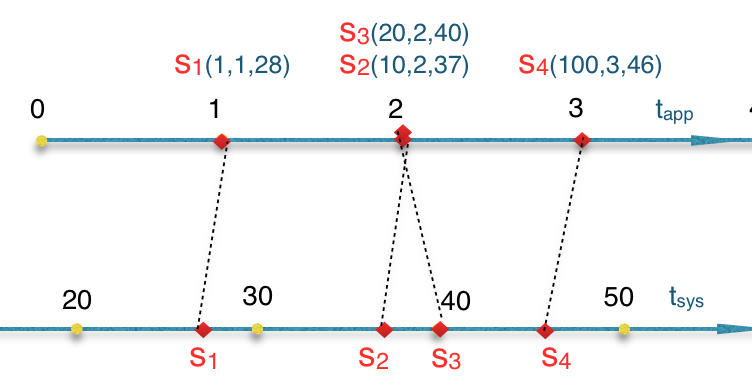
\includegraphics[width=0.5\textwidth]{tuple-driven}
\caption{tuple-driven}
\label{fig:tuple-driven}
\end{figure}
	
	\item \textbf{Batch-driven} execution model, followed by Coral8, mentioned in SECRET\citep{Botan:2010} descriptive model
\end{itemize}. In this model, each tuple is assigned an batch-id. Every tuple which belong to a batch must have the same timestamp, but 2 separate tuple with the identical timestamp may belong to two different batches. As we can see, batch-driven model is in between of tuple-driven and time-driven model (Figure~\ref{fig:executionModel}). Assuming that at a given application timestamp $\tau$, the system receives 5 tuples ${<v_1,\tau>,<v_2,\tau>,<v_3,\tau>,<v_4,\tau>,<v_5,\tau>}$. Time-driven model treats them as simultaneous tuples with no difference. Tuple-driven considers them as 5 concrete tuples in strict order. And batch-driven model may divide them into 2 batches $\{<v_1,\tau>,<v_2,\tau>,<v_3,\tau>\}$, $\{<v_4,\tau>,<v_5,\tau>\}$ depending on window specification.


	\begin{figure}[htbp!] 
\centering    
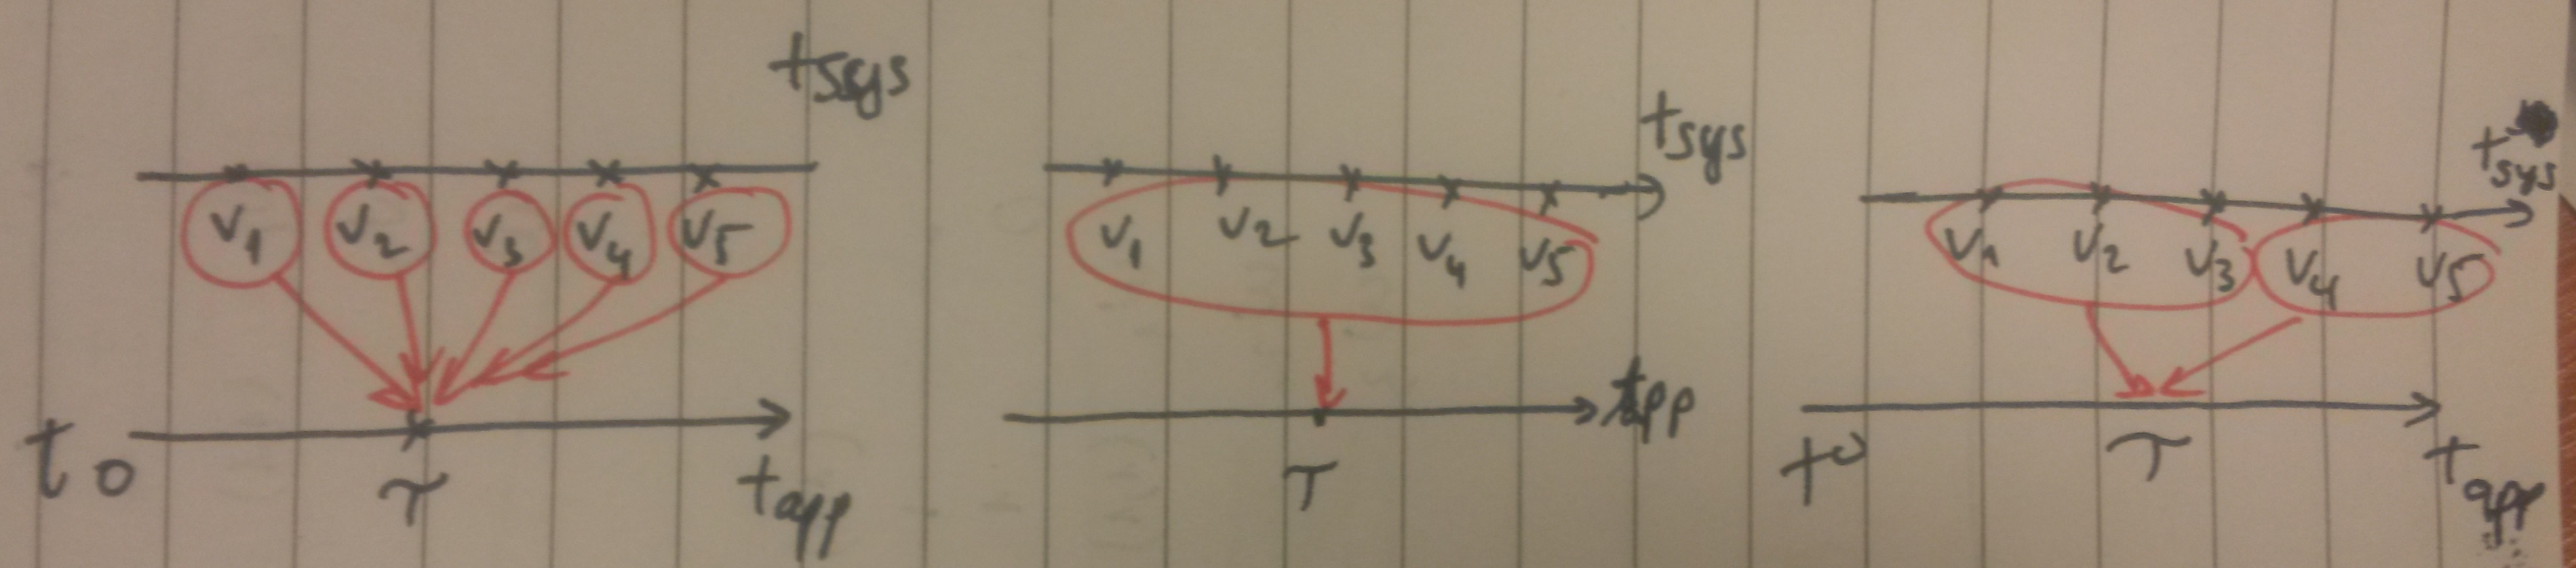
\includegraphics[width=1\textwidth]{executionModel}
\caption{Execution Model}
\label{fig:executionModel}
\end{figure}


We extends the examples \citep{Dindar:2013} with Flink implementation in order to demonstrate that system with different execution model may produce different output , even with the same input and query. 
\begin{enumerate}

\item Example 1: differences in window constructions
Given \textit{Instream} stream with schema $S(time, value)$. Consider a query which continuously computes the average value of tuples in a time-based tumbling window of size 3.
\begin{align*}
Instream(time,value) &= \{(10,10),(11,20),(12,30),(13,40),(14,50),\\
&\qquad (15,60),(16,70),...\} \\
Oracle\, CEP\, (avg)		&= \{(20), (50),...\} \\
Flink\, (avg)			&= \{(15), (40),...\} \\
\end{align*}

Obviously, Oracle CEP constructs the first window with first 3 tuples whereas Flink picks first 2 tuples only. The second window , they both take next 3 tuples. We implement the test on Flink with default configuration, however we are able to customize the upper bound of the first window ($startTime = 12$)so that it produces the same result as Oracle CEP.


\item Example 2: differences in window evaluations

Consider a query which continuously computer the average value of tuples over last 5 second once every 1 second (time-based window of size 5s that slides by 1s)

\begin{align*}
Instream(time,value) 	&= \{(30,10),(31,20),(36,30),...\} \\
Oracle\, CEP\, (avg)		&= \{(10), (15),(20),...\} \\
Flink\, (avg)			&= \{(10), (15), (15), (15), (15), (20),...\}\\
Coral8\, (avg)			&= \{(10), (15),(20),...\}			
\end{align*}

Flink produced a different result than Oracle and Coral8.
In Oracle and Coral8, a new window is emitted for invoking the average operator only when the window content's change; whereas in Flink, it emits a new window every second as the sliding progress , even if the content does not change. The state of window is depicted on Figure ~\ref{fig:winEvaluation}
\begin{figure}[htbp!] 
\centering    
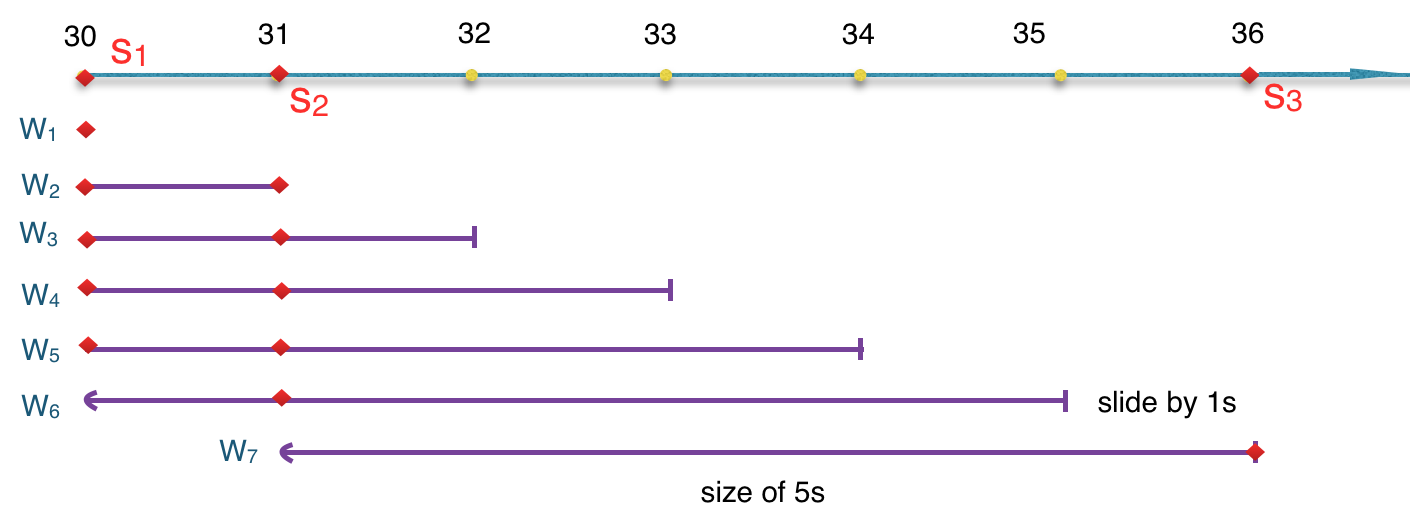
\includegraphics[width=0.7\textwidth]{winEvaluation}
\caption{Window State}
\label{fig:winEvaluation}
\end{figure}

Remember that window closes at upper boundary and opens at lower boundary so that in window $W_6$ cover from $t=35$ to right after $t=30$ will exclude tuple $(30,10)$. Similarly, $W_7$ excludes tuple $(31,20)$


\item Example 3: differences in processing granularity

Consider a query which computes the average value of tuples over a tuple-based tumbling window of size 1 tuple.
\begin{align*}
Instream(time,value) 	&= \{(10,10),(10,20),\\
						&\quad (11,30),\\
						&\quad (12,40),(12,50),(12,60),(12,70),\\
						&\quad (13,80),...\} \\
Oracle\, CEP\, (avg)		&= \{(20), (30),(70),(80)...\} \\
Flink\, (avg)			&= \{(10), (20), (30), (40), (50), (60),(70),(80)...\}\\
Coral8\, (avg)			&= \{(10), (20), (30), (40), (50), (60),(70),(80)...\}
\end{align*}

Oracle CEP implements time-based execution model so that it reacts to each application timestamp. If there are multiple simultaneously tuple arrive, it will pick one of them non-deterministically to construct the window , since window size is 1. In other hand, Flink and Coral8 react to every tuple arrival so that they emit new 1-tuple-size tumbling window for every tuple.

\end{enumerate}

tuple: each tuple arrival cause a system to react
time: the progress of tapp cause a system to react
batch:  where either a new batch arrival or the progress of tapp cause a system to react


http://blog.mikiobraun.de/2014/01/apache-spark.html


\section{Policy-based Window Semantics}


Flink constructs windows based on parameters in specification. Currently Flink does not support Predicate Window so that two of most critical parameters are to notify when system should trigger new windows (indicating the lower bound of window) and when system must end the window (indicating the upper bound of window) and emit it to window stream. For that purpose, Flink implements a mechanism called \textit{"Policy-based windowing"}. It is a highly flexible way to specify stream descretization. It has two independent policies corresponding to open and close window: Trigger and Eviction Policy.
To demonstrate the concepts of two policies, let's consider the scenario with \textit{StockTick} stream: check every 10 minutes the total transaction volume of all transaction last 30 minutes. In other words, in every 10 minutes create a new window to cover all the transactions in last 30 minutes. The syntax in Fink:

\begin{verbatim}
StockTick.window(Time.of(30, MINUTES))
		 .every(Time.of(10, MINUTES)).sum(Quantity)
\end{verbatim}

\begin{enumerate}

\item \textbf{Eviction Policy}: define the length of a window. The length is passed in to \textit{window(...)} function. It could be the time interval, number of tuples and delta function with threshold (in case of delta window).
We formalize the concept of window due to its size

\begin{defi}
A time-based window $W_{t} = (l,u,\omega)$ over a stream $S$ is a finite subset of  $\mathbb{S}$ containing all data elements $s \in \mathbb{S}$ where $l , u, \omega \in \mathbb{T}$ and$l < s.t \leq u$. The length of window in time unit is $\omega = u-l$
\end{defi}
Notice that in a time-based window, $s.t$ can be tuple's application or system timestamp depending on query. There are maybe many simultaneous tuples with an identical $t_{app}$. However, there is at least one arriving tuple at a given $t_{sys}$. The second point is that $W_t$ open at $t = l$, it does not include tuple at this time instant.

\begin{defi}
A count-based window $W_{c} = (l,u,\omega_c)$ over a stream $S$ is also a finite subset of  $\mathbb{S}$ containing all data elements $s \in \mathbb{S}$ where $l,u \in \mathbb{T}$, $\omega_c \in \mathbb{N}$ and $l \leq s.t_{sys} \leq u$. The length of window is the number of tuples in interval time $(l, u]$, i.e., $\omega_c = | {s \in \mathbb{S}(t_{sys}): l < s.t_{sys} \leq u}|$
\end{defi}
The count-based window $W_{c}$ is independent from application timestamp $t_{app}$. It is related to system timstamp $t_{sys}$ which indicate tuple's order in stream. 


\item \textbf{Trigger Policy}: In general, it defines window slide or the distance between 2 consecutive windows. On above example , trigger policy states that from beginning, system must trigger a new window every 10 minutes. No other window would be triggered in between.

Supposed that we have 2 consecutive windows $W^1 = (l_1, u_1, \_)$ and $W^2 = (l_2, u_2, \_)$  where $l_1 < l_2$. There is no window $W^1 = (l_3, u_3, \_)$ such that $l_1< l_3 < l_2$.
\begin{defi}
The distance or slide between 2 window $W^1$ and $W^2$ is the distance between two of their upper-bound tuple as
\begin{itemize}


\item  A time-based slide $\beta_{t} = u_2 - u_1$.  
\item A count-based slide $\beta_{c} = |{s \in \mathbb{S}(t_{sys}): u_1 < s.t_{sys} \leq u_2}| $ 

\end{itemize}

\end{defi}

\end{enumerate}

There is a correlation between window size and slide size  conforming to the movement type of windows.
\begin{itemize}
\item Sliding window: $\omega > \beta$ or $n > e$
\item Tumbling window: $\omega = \beta$ or $n = e$
\item Jumping window: $\omega < \beta$ or $n < e$
\end{itemize}

However, Flink allow to mix between time-based trigger policy with count-based eviction policy and vice versa. For example,
calculate sum of quantities of last 100 transactions every 1 hour.
\begin{verbatim}
StockTick.window(Count.of(100))
		 .every(Time.of(1, HOURS)).sum(Quantity)
\end{verbatim}

\section{The execution models in Flink}
We present here the execution models of Flink Stream Processing engine. Tick model specifies how the engine reacts to new tuple arrival while Window Construction show the way Flink constructs and emit the windows based on window specifications. There are pretty many reviews on window construction ... However, none of them give the full description in the case that we mix up time-based and time-based specification for window size and slice.  //TODO



%\begin{verbatim}
%
%		boolean isTriggered = false;
%
%		if (triggerPolicy.notifyTrigger(input)) {
%			emitWindow();
%			isTriggered = true;
%		}
%
%		evict(input, isTriggered);
%
%		collector.collect(windowEvent.setElement(input));
%		bufferSize++;
%
%\end{verbatim}

Window Buffer \textit{wb} is a linking list contain tuples with composite type $IN$



\begin{equation}
	t = 
	\begin{cases}
		t_{sys} \qquad if\,t_{app} = None\\
		   \\
		t_{app} \qquad\qquad\qquad otherwise
	\end{cases}
\end{equation}

$size_{t}(wb) = wb.last.t - wb.first.t$

$size_c(wb) = wb.length()$


\begin{algorithm}
\caption{Process new arrived tuple}
\label{algorithm:processNewTuple}
The first step, before processing a new arrived tuple, check if a current window buffer should be emit. If yes, copy the current window buffer to a window object and put to Windowed Stream. The second step, calculating which tuples should be evicted if the current window buffer appends new arrived tuple. There are two separate case for time-based and tuple-based window. The third step, evicting those tuples and appending new arrived tuple.


\algrenewcommand\algorithmicfunction{\textbf{class}}
\algrenewcommand\algorithmicprocedure{\textbf{method}}
  \begin{algorithmic}[1]
  	\Require {$wb$: the current window buffer}
  	
  			{$\omega_t$: size of window in time interval }
  			
  			{$\omega_c$: size of window in tuple count }
    %\Function{Mapper}{}
    \Procedure{processNewTuple}{$\textrm{newTuple }: IN$}
    
    \If{$\textsc{notifyTrigger}(newTuple) \textrm{ \& } size_c(wb) > 0$} \Comment{ trigger new window}
    		\State $\textrm{window} \gets \textrm{wb}$
    		\State $\textsc{Emit}(\textrm{window})$ \Comment {emit to Windowed stream}
    \EndIf
    
    \If{$\textrm{window is time-based}$}
    		\State $ evict_t \gets size_t (\textrm{wb.append(newTuple)}) - \omega_t$
    
    		\If{$evict_t > 0$} \Comment {remove old tuples}
    			\State $ \textrm{lastEvictedTimestamp} \gets wb.first.t + evict_t - 1$
    			\ForAll{element $e$ in window buffer $wb$}
    				\If {$e.t \leq \textrm{lastEvictedTimestamp}$}
    					\State $wb.remove(e)$
    				\EndIf
    			\EndFor
    		\EndIf
    \Else \Comment{window is count-based}
    		\State $evict_c \gets size_c(\textrm{wb.append(newTuple)}) - \omega_c$
    		\If{$evict_c > 0$} \Comment {remove old tuples}
    			\For {$i \gets 1, evict_c$}
    				\State $wb.removeFirst()$
    			\EndFor
    		\EndIf
    \EndIf
    
   	\State $wb \gets wb.append(newTuple)$ \Comment {add new tuple to current window buffer}
    
    
    \EndProcedure
    %\EndFunction
  \end{algorithmic}
  




\end{algorithm}


\begin{algorithm}
\caption{Whether system should trigger a new window }
\label{algorithm:notifyTrigger}
When a new tuple has arrive, system check whether the current window buffer reached the point where distance of 2 windows is equal to slide size or not. The new tuple is not really appended to buffer, use it for qualifying purpose only.

\algrenewcommand\algorithmicprocedure{\textbf{method}}
\begin{algorithmic}[1]
  	\Require {$\beta_c$: count-based slide size}
  	
  			{$\beta_t$: time-based slide size }

  			{$lastUpperBound$: timestamp of upper boundaries of previous window}
    %\Function{Mapper}{}
    \Procedure{notifyTrigger}{$\textrm{newTuple }: IN$}
    
   
    
    \If{$\textrm{slide is time-based}$}
    		\If{$(\textrm{newTuple.t} - lastUpperBound) > \beta_t$}
    			\State $\textrm{lastUpperBound} \gets \textrm{lastUpperBound} + \beta_t$
    			\State $\textrm{return true}$
    		\Else
    			\State$\textrm{return false}$
    		\EndIf
    
    \Else \Comment{window is count-based}
    		\If{$\textrm{counter} \geqslant \beta_c $}
    			\State $\textrm{counter} \gets 1$
    			\State $\textrm{return true}$
    		\Else
    			\State $\textrm{counter} \gets \textrm{counter} + 1$
    			\State $\textrm{return false}$
    		\EndIf
    	\EndIf
    
    
    \EndProcedure
    %\EndFunction
  \end{algorithmic}
\end{algorithm}


\subsection{Tick Model}
As we mentioned in \ref{Heterogeneity}, there are three common Tick execution models\citep{Dindar:2013} implemented in various systems. STREAM and Oracle CEP implements time-driven model which react once to all tuples with the identical application timestamp. Coral 8 with batch-driven model takes action on an atomic batch which may contain multiple tuples with the same batch-id. Flink and StreamBase with tuple-driven model actively trigger actions on every new arrived tuple. Tuples are strictly totally ordered based on its system-assigned timestamp. We describe a procedure taking on a recent arrived tuple in method \textit{processNewTuple}  (in algorithm\ref{algorithm:processNewTuple}). 
System takes action on new tuples one by one due to its moment of arrival. 
Basically, Flink employs a linked list as a window buffer to temporarily store a queue of arrived tuples. New tuple will be added to window buffer whereas old tuples will be removed from window buffer according to eviction policy.

Whenever a new tuple has arrived, the procedure is as following:
\begin{itemize}
\item \textbf{Step 1:} The system checks whether the stream reached the point where it should emit the current window buffer to windowed stream and trigger a new window. The condition to trigger a new window is represented in method \textit{notifyTrigger} (in algorithm \ref{algorithm:notifyTrigger}). If the condition is satisfied and window buffer is not empty, system will emit the current window buffer to discretized Windowed Stream for later computation.  

In method \textit{notifyTrigger}, system decides to trigger a new window according to trigger policy defined in window specification. 
Supposed that the previous emitted window is $W^1$, the current window buffer is $wb$, and new arrived tuple $s$.
If the distance between $W^1$ and $\textrm{wb} \bigcup \{s\}$ start exceeding slide size $\beta$ (defined in window specification), system confirms the trigger point and reset the slide measurement:
\begin{itemize}
\item If the slide is time-based, set timestamp of new upper boundaries as \textit{lastUpperBound}
\item If the slide is count-based, reset counter to 1

\end{itemize}

Notice that system has not inserted new tuple to window buffer yet, but at last step.

\item \textbf{Step 2: }evict old tuples in window buffer.
Supposed that system adds new tuple to window buffer, system evicts a number of oldest tuples so that size of the buffer does not exceed pre-defined window size $\omega$. This eviction policy is activated whenever a new tuple has arrived to ensure that window buffer size  never exceed $\omega$
\begin{itemize}
	\item if the window is time-based, time interval cover the window is not bigger than $\omega_t$
	\item if the window is tuple-based, number of tuples in the window does not exceed $\omega_c$
\end{itemize}
\item \textbf{Step 3:} officially insert new tuple to window buffer.
\end{itemize}

In short, we figure out some crucial properties of Tick model in Flink
\begin{itemize}
\item Flink implements tuple-driven model reacting to every new arrived tuple.
\item The eviction policy is to keep size of window buffer shrink shrunk to pre-defined window size $\omega$
\item One is able to mix up different type of window and slide size. For instance, tuple-based window slide by time interval.
\end{itemize}



\subsection{Window Constructions}
We are able to define window and slide size based on application timestamp, system timestamp or number of tuple. Therefore, we have 9 ways to construct a basic window with combination of window and slide size.


\subsubsection{Upper boundary}
In time-based slide,  supposed that $u_1$ is  the upper boundary of the first window. 
The upper boundary of the $k$th window is $u_k = u_1 + k.\beta_t$

\begin{figure}[htbp!] 
\centering    
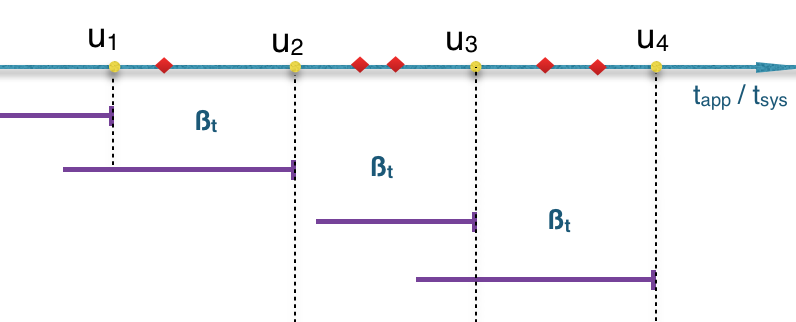
\includegraphics[width=0.5\textwidth]{timebased_slide}
\caption{time-based slide}
\label{fig:timebased_slide}
\end{figure}

In count-based slide, supposed that $u_1$ is the system timestamp of last element of the first window, the last element $s<v,_,t_k>$ of the $k$th window must satisfies $|{s \in \mathbb{S}(t_{sys}): u_1 < s.t_{sys} \leq u_2}| = n.\omega_c$

\begin{figure}[htbp!] 
\centering    
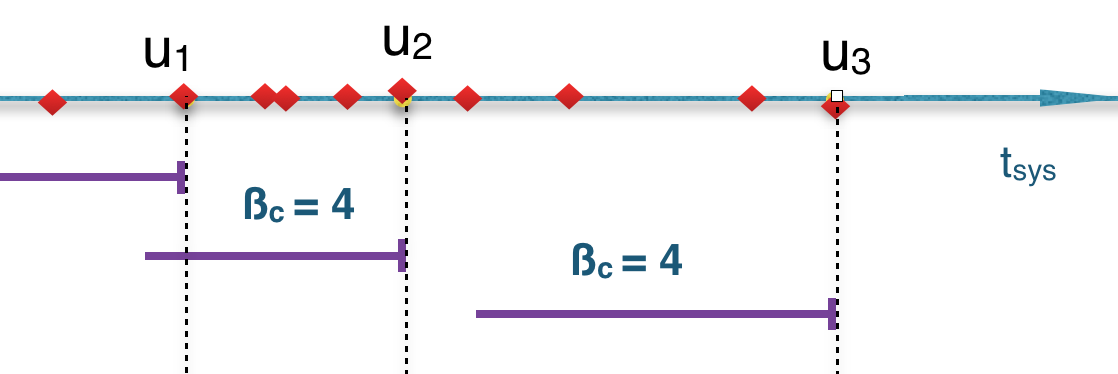
\includegraphics[width=0.5\textwidth]{countbased_slide}
\caption{count-based slide}
\label{fig:countbased_slide}
\end{figure}

\subsubsection{Lower boundary}

In time-based windows, windows are defined in terms of of timestamp. Supposed that we know the upper bound $u_k$ of the $k$ window. The lower bound $l_k = max(0, u_k - \beta_t)$

\begin{figure}[htbp!] 
\centering    
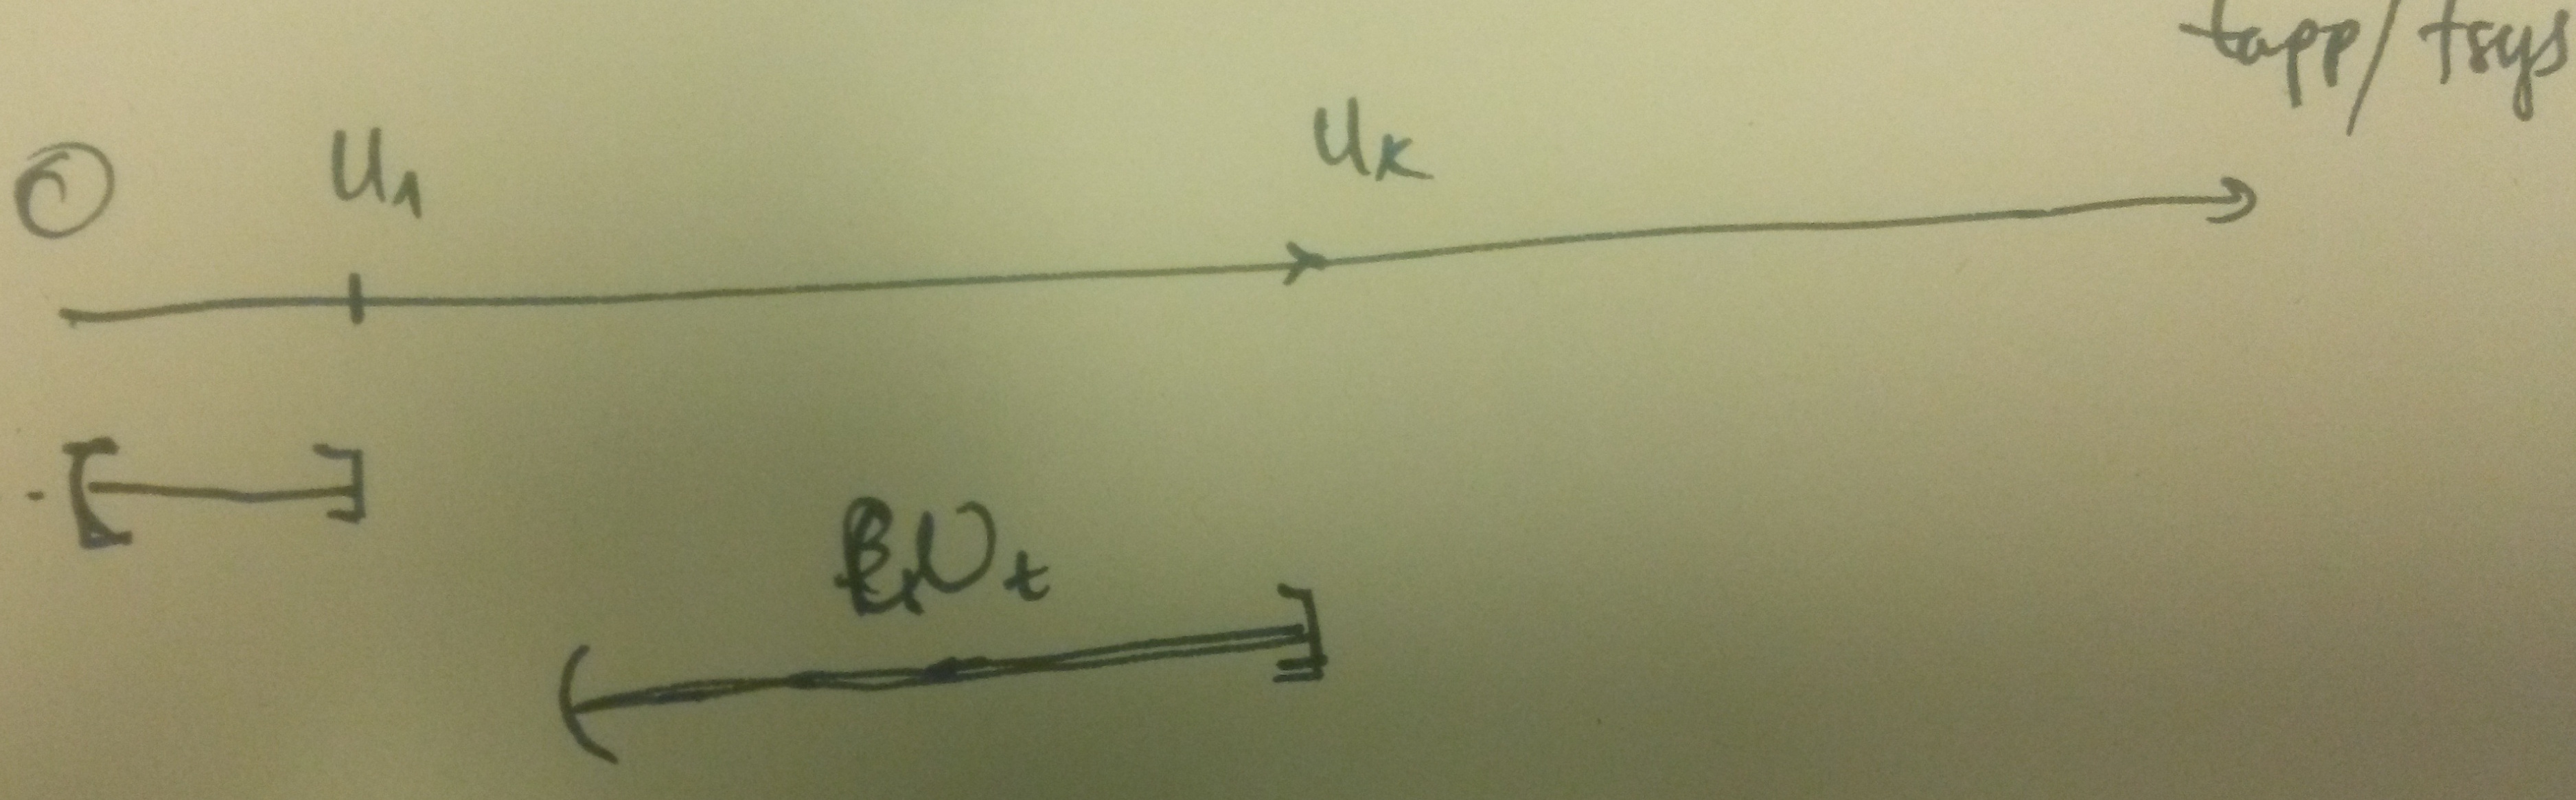
\includegraphics[width=0.5\textwidth]{timebased_window}
\caption{time-based window}
\label{fig:timebased_window}
\end{figure}

\begin{itemize}
\item Using application timestamp. The window content is $W = \{s:<v, t_{app},\_> \in \mathbb{S} \wedge max(0, u_k - \omega_{t_{app}}) < t_{app} \leq u_k\}$ where $u_k$ is upper boundary of window in application timestamp unit


\item using system timestamp. The window content is $W = \{s:<v,\_, t_{sys}> \in \mathbb{S} \wedge max (0, u_k - \omega_{t_{sys}}) < t_{sys} \leq u_k\}$ where $u_k$ is upper boundary of window in system timestamp unit
\end{itemize} 


In count-based windows, the scope of window is defined in terms of number of tuples. Thus, given the last tuple $s:<v, \_, u_k>$ of the window. The window content is 
$W=\{s:<v, \_, t_{sys}> \in \mathbb{S} \wedge t_{sys} \leq u_k \wedge  |\{<v,\_,t'_{sys}> \in \mathbb{S} : t_{sys} \leq t'_{sys} \leq u_k\}| \leq \omega_c \}$

\begin{figure}[htbp!] 
\centering    
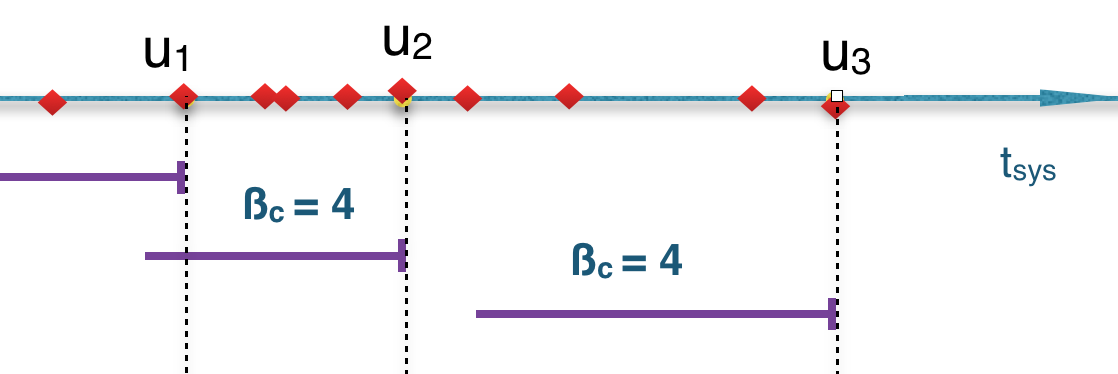
\includegraphics[width=0.5\textwidth]{countbased_slide}
\caption{count-based slide}
\label{fig:countbased_slide}
\end{figure}


\subsubsection*{In case of partitioned group within window}


%*******************************************************************************
%****************************** Second Chapter *********************************
%*******************************************************************************

\chapter{FlinkCQL- Queries over Data Stream}

\ifpdf
    \graphicspath{{Chapter4/Figs/Raster/}{Chapter4/Figs/PDF/}{Chapter4/Figs/}}
\else
    \graphicspath{{Chapter4/Figs/Vector/}{Chapter4/Figs/}}
\fi

\section{Fundamental of query languages}
\subsection*{Query}

A query is a request telling system what to do in order to retrieve or alter desired information stored or processed by system. For instances, asking ``How many products are sold today?''. Queries over data stream and in a traditional DBMS have a lot in common; however, due to characteristic of continuousness in data stream, we may classify a query as one-time query or continuous query \citep{Terry:1992} \citep{Babcock:2002}. 
\begin{itemize}
	\item \textbf{One-time queries} are evaluated once over data set at a given time instant, and terminated after returning its result. This is also called \textit{passive query} \citep{SmartVotex:2011} since system require queries and passively waits for users to issue these queries before executing. 
	\item \textbf{Continuous queries}, in contrast, get evaluated continually as new data arrives to the observed stream. System continuously delivery new results  over time according to the snapshot or state of data stream seen so far. Thus the output of queries is not a single result, but rather new streams of results for further operators if desired. Obviously, continuous queries really fit to user's requirements to observed data streams till its end. 
\end{itemize}


\subsection*{Query Language}
Queries are expressed in terms of some query languages. They provide for users and programmers a very general way to specify data selections, projections, combination, computation and so on over data set/stream. In the meanwhile, users can send the queries using either imperative or declarative language.

\subsubsection*{Imperative vs. Declarative language}
\begin{itemize}
	\item \textbf{Imperative language} requires users to define explicitly step by step \textbf{how} code should be executed to get \textbf{what} they want. They need to break the program into sequences of commands in particular order for the system to perform. Actually, many existing programming languages are imperative supporting \textit{assignment}, \textit{for-loop}, \textit{if-else} statements and so on to construct a complete program. For example, assuming that \textit{StockTick} is a  list of stock transactions,  to filter through \textit{StockTick} to get all stock transactions from `NYSE' only: 
\begin{lstlisting}
	function getTransFromNYSE {
		var fromNYSE = []
		for (var i = 0; i < StockTick.length; i++) {
			if (StockTick[i].Exchange == "NYSE")
				fromNYSE.add(StockTick[i])
		}
	}
\end{lstlisting}
	\item \textbf{Declarative language}, like SQL or LINQ, users just specify \textbf{what} they want - which sort of data, which transformation they want it to be afterwards, but \textbf{not how} to achieve the result. The corresponding declarative program for previous examples is written in SQL language as below:
	\begin{verbatim}
		SELECT * from StockTick where Exchange = "NYSE"
	\end{verbatim}
\end{itemize}

There are several advantages of declarative over imperative language \citep{Martin:2014}:

\begin{itemize}
	\item Declarative language is typically more concise , more friendly and easier to work with. For instance, comparing 2 previous programs, the former has 7 lines of code while the latter goes with 1 line. According to \citep{Ronnie:2015}, Java program is typically 50 times less compact than SQL query for the same purpose. Generally, that is because they have different level of abstraction. Declarative language already hides complicated implementation details. It makes the program much more simpler but possible for system to introduce underneath improvement without any impact on queries.
	\item Declarative languages, for example SQL, HTML,  are usually followed a set of standard syntax which make it more limited in functionality, give the system more room for automatic optimization. 
	\item In terms of parallel execution environment, declarative language like SQL has a better chance to be executed faster. Imperative code instructs its sequence of operators to be performed in a certain order so that it is really hard to parallelize programs across distributed system. In the other hand, declarative queries are more atomic to be implemented in parallel if appropriate.
\end{itemize}

\subsection*{FlinkCQL - a SQL-like dialect for Flink Streaming Processing}
Recently, there are 2 common forms of declarative language applying to data query: SQL and LINQ. However, we decide to extend SQL syntax for our continuous query language due to several advantages:
\begin{itemize}
	\item Traditional database model and data stream model are distinguished but till share many common features and operators. Since, SQL is well-designed for handle data in batch mode, extending it to handle data-in-motion in data stream model is a possible incremental approach to quickly define language with less effort.
	\item SQL is so common and recognized by most of developers. Therefore, extended SQL languare would not challenge them to learn and master it.
	\item SQL is a standard adopted by most of relational database systems. As a result, their syntax is well-designed and quality-guaranteed to use. Moreover, parsers, visualizers and composers for SQL are readily available to extend.
\end{itemize}

%//TODO:http://www.sqlstream.com/blog/2015/03/why-we-need-sql-for-real-time-streaming-analytics/

	
%\subsubsection*{LINQ}
%https://www.linqpad.net/WhyLINQBeatsSQL.aspx
%http://pankajtiwarii.blogspot.hu/2012/09/advantages-and-disadvantages-of-linq_3.html

%Despite its power, LINQ doesn't deprecate SQL. It takes more than 95 percents of the querying brunt, but you still sometimes need SQL for:

%Hand-tweaked queries (especially with optimization or locking hints)

%Queries that involve selecting into temporary tables, then querying those tables

%Predicated updates and bulk inserts

%\subsubsection*{Visual languages} \citep{Henrique:2014}


There are several properties of data stream which we take into account when extending SQL to FlinkCQL:

\begin{itemize}
	\item \textbf{Language closure}: In Relational algebra, closure property states that each operation takes one or more input relations and return an output relation. Thanks to this property, we are able to write nested relational expression. For example, a nested \textit{Select} query in \textit{From} clause or in \textit{Insert} statement. 
	Therefore, to give more room for user to create a complex query at once, FlinkCQL should support nested queries and pay attention to the closure property. 
	
	\item \textbf{Windowing} FlinkCQL should allow to define window specifications and  implement related operators. There is no doubt that Windowing is a essential technique in Stream Processing, not only because it is a mean to find a approximate query answering but also because it is strongly inspired from users' requirements. 
	
	\item \textbf{Blocking and Non-blocking operators} Naturally, blocking operation is not applicable to data stream.  According to~\citep{Babcock:2002}:
	\begin{defi}
		A blocking query operator is a query operator that unable to produce the first tuple of its output until it has seen its entire input.
	\end{defi} 

Sorting, joining or aggregation such as SUM, COUNT, MIN, MAX, AVG are examples of blocking operators. Obviously, the end point of a data stream is nearly unpredictable so that these blocking operators are not very suitable to the data stream model. 

In contrast, non-blocking operators, which can produce some tuples of output before it has detected the end of input, can be applied on data stream. Some of non-blocking operators such as projection, selection, partition, merge, split stream, can process new tuples on-the-fly without storing any temporary results~(stateless).

However, it would be a huge drawback if blocking operators is missing in query language since they are very common for simple analytics. Fortunately, since a window contains a finite set of tuples, we are able to implement a blocking operators on each window in the lieu of the whole stream. 

In short, blocking operators are possible to query on Windows only  while non-blocking operators can be applied on both concrete data streams or windows. 
	
\end{itemize}

I propose FlinkCQL and describe its syntax on session~\ref{language} then its semantic  on session~\ref{semantic}

// TODO: stronger statement


%//TODO
%In the streaming literature, query language model a stream as a representation for an infinite append-only relation. The append-only stream model effects the following limitations\citep{Ghanem:2008}
%\begin{itemize}
%\item It limits the applicability of the language since the append-only models cannot represent streams from the various domain( e.g., the update streams or streams that represent concatenation of the states of a fixed size relation).
%\item The append-only stream model limits the types of queries that the language can express since only non-blocking queries can produce append-only streams as output
%\item The semantics of query composition in the append-only stream model is complex and the meaning of the composed queries is difficult to understand.
%\end{itemize}

% //TODO: reference

%Query \citep{Babcock:2002} 

%Query : Smart Votex , page 2

%Window Specification over Data Streams.pdf

%[Stream] Evaluate CQL

%Designing\_Data\_Intensive\_Applications.pdf



%\section{Fundamental Features}

%\begin{itemize}
%\item Stream-oriented Query Languages and Operators
%	\begin{itemize}
%		\item Language closure
%		\item Windowing
%		\item Correlation
%		\item Pattern Matching
%	\end{itemize}
	
%\item Fundamental of Stream Processing : page 110
%	\begin{itemize}
%		\item Compositional elements
%		\item Declarative operators
%		\item Expression language
%		\item Type System
%		\item Windowing
%		\item Standard operators and adapters
%		\item Modularity
%		\item Configuration
%		\item Extensiblity
%	\end{itemize}
%\end{itemize}


\section{Continuous Query Language} \label{language}

\subsection{Data Type}

FlinkCQL supports numbers of data types including numeric types (\textit{Byte}, \textit{Short}, \textit{Int}, \textit{Long}, \textit{Float}, \textit{Double}), \textit{Boolean}  type, string types (\textit{Char}, \textit{String}), deta type (\textit{Datetime}) with detailed descriptions in (Table~\ref{table:Data Type})


\begin{table}[h]
\caption{Data Type}
\centering
\label{table:Data Type}
\setlength\extrarowheight{5pt}
\begin{tabular}{||>{\centering\bfseries}m{1in} |>{\centering}m{3in}  |>{\centering\arraybackslash}m{2in}||}
\hline
%\rowcolor[HTML]{ECF4FF} 
%{\color[HTML]{ECF4FF} \textbf{Scala Type}} & {\color[HTML]{ECF4FF} \textbf{Flink Type}} & {\color[HTML]{ECF4FF} \textbf{Viewable as}} \\ \hline
\textbf{FlinkCQL Type} & \textbf{Description}  & \textbf{Convertable to} \\ \hline\hline
                    String  & A sequence of Chars                               &  \\ \hline
                    Boolean	& Either the literal true or the literal false			               &   \\ \hline
                   Char		& 16 bit unsigned Unicode character. Range from U+0000 to U+FFFF			 &  Byte, Short, Integer, Long, Double\\ \hline
					Byte		 & 8 bit signed value. Range from -128 to 127          	                   & Short, Integer, Long,Float, Double \\ \hline
					Short	& 16 bit signed value. Range -32768 to 32767			               & Integer, Long, Float, Double\\ \hline								
					Int		& 32 bit signed value. Range -2147483648 to 2147483647			 & Long, Float, Double\\ \hline
					Long		& 64 bit signed value. -9223372036854775808 to 9223372036854775807	 		                     & Float, Double \\ \hline								
					Float	& 32 bit IEEE 754 single-precision float			                    & Double \\ \hline
					Double	& 64 bit IEEE 754 double-precision float			                  &   \\ \hline							
	Datetime				&     'YYYY-MM-DD HH:MM:SS' format. The supported range is '1000-01-01 00:00:00' to '9999-12-31 23:59:59'               &        	\\ \hline           							           							           							           							           
\end{tabular}
\end{table}



\subsection{Data Definition Language (DDL)}
We utilize Extended Backus–Naur Form (EBNF) to make a formal descriptions of FlinkCQL. To understand the syntax, there are some EBNF notations to know
\begin{itemize}
	\item $\textbf{[...]}$ : Expression inside squared brackets is \textit{optional}
	\item $\textbf{\{...\}}$ : Expression, which is wrapped by curly braces, is omitted or repeated. 
	\item $\textbf{|}$ : alternation (or)
\end{itemize} 
Moreover, be aware that \textit{ident} stands for \textit{Identifier} which is recognized as name of schema, stream, data attribute and so on.
\subsubsection{Create Schema}

%\setlength{\grammarparsep}{20pt plus 1pt minus 1pt} % increase separation between rules
\setlength{\grammarindent}{12em} % increase separation between LHS/RHS 

\begin{grammar}

<schema statement> ::= CREATE SCHEMA <schema ident> \\
(<named schema ident>|<anonymous schema>) \\
  { }[EXTENDS <parent schema ident>]

<anonymous schema> ::= `(' <typedAttribute> \{`,' <typedAttribute>\}`)'

<typedAttribute> ::= <attribute ident> <data type>

\end{grammar}
	
Similar to CREATE TABLE statement in SQL, we are able to identify a schema of stream tuples. Each schema consist of name followed by list of data attributes (the combination of attribute identifier and its data type). For example, we create schema for \textit{StockTick} stream:
\begin{verbatim}
CREATE SCHEMA StockTickSchema (symbol String, sourceTimestamp Long, 
price Double, quantity Int, exchange String)
\end{verbatim}

We extends the grammar so that a schema can be referenced or extended to another schema. For examples, in below examples, \textit{StockTickSchema2} is referencing to previous \textit{StockTickSchema} so that they own a similar set of attributes. Meanwhile, \textit{StockTickSchema3} extends from it to have one more attribute (\textit{"id"})
\begin{verbatim}
CREATE SCHEMA StockTickSchema2 StockTickSchema
CREATE SCHEMA StockTickSchema3 (id Int) EXTENDS StockTickSchema
\end{verbatim}

\subsubsection{Create Stream}
	
					
\begin{grammar}
<Stream statement> ::= CREATE STREAM <schema ident> \\		(<named schema ident>|<anonymous schema> ) \\
{ }[<source>]

<source> ::= (AS <derived source>) | ( SOURCE <raw source>)

<derived source> ::=  <stream ident>| <subSelect>

<raw source> ::= 
				SOCKET `('<host>, <port> [, <delimiter>]`)'
					\alt FILE `('<file path> [, <delimiter>]`)'
\end{grammar}

A stream cannot be queried unless it is registered with a schema, simply because system require users to specify name of attributes for expression in most of cases. For this reason, we allow to entitle a stream to its schema using CREATE STREAM statement. Except for the reserved keywords, the statement consists of 3 parts. Stream name declaration is followed by schema definition and source of stream. Its schema can be recalled from a previously-defined named schema such as \textit{StockTickSchema}. 
\begin{verbatim}
CREATE STREAM StockTick StockTickSchema;
\end{verbatim}

One also has abilities to define new schema with a set of attribute name and type. In this case, the stream and its schema share the same name.
\begin{verbatim}
CREATE STREAM StockTick (symbol String, price Double, quantity Int)
\end{verbatim}

The last part is optional source of stream. Recall that we have two kind of stream representations: base stream and derived stream. \textit{<raw source>} clause indicates that this is a base stream obtained through a network connection (\textit{<host>, <post>}) or from a text file. For instance, \textit{StockTick} stream originates from host \textit{98.138.253.109} via port \textit{2000}

\begin{verbatim}
	CREATE STREAM StockTick StockTickSchema 
	SOURCE SOCKET ("98.138.253.109", 2000)
\end{verbatim}

Derived stream may come from another existing stream or output of a query and its operators. \textit{<derived source>} clause indicates these two possibilities. For example, we register a new stream \textit{StockPrice} which is derived from \textit{StockTick} but pay attention to stock symbol and its price only
\begin{lstlisting}
	CREATE STREAM StockPrice (symbol String, price Double) AS
	SELECT symbol, price 
	FROM StockTick
\end{lstlisting}


\subsection{Data Manipulation Language (DML)}

\subsubsection{Insert}

\begin{grammar}
<insert statement> ::= INSERT INTO <stream ident> [AS] 
							(<stream ident> | <subSelect>)
\end{grammar}
% <merge>

In CREATE STREAM statement, stream identifier and its schema definition are required but its source is optional. It means that registered stream could attached its source later when it is available. In this case, we take the advantage of INSERT statement to complete stream registration procedure. However, we support INSERT statement for derived stream only. It naturally makes sense because a base stream is concrete and should be permanently registered from beginning. We then can insert it into other stream if possible.
Keep in mind that INSERT statement is a complementary to CREATE STREAM statement in case \textit{<source>} is missing. It will not work for a stream identifier which already refer to a real stream source.

\begin{verbatim}
	CREATE STREAM StockTick StockTickSchema;
	INSERT INTO StockTick AS stockStream;
\end{verbatim}


\subsubsection{Merge}
\begin{grammar}
<merge statement> ::= MERGE <stream ident> `,' <stream ident> {`,'<stream ident>}
\end{grammar}

One of data stream properties is that data are emitted by a variety of external sources. It is cumbersome to write a similar query for each of substream. To eliminate this duplication, Flink allows to merge various registered stream with same Schema into one. For example, we integrate all StockTick from several Exchange into one:
\begin{verbatim}
	MERGE stockTickFromNYSE, stockTickFromAMEX, stockTickFromNASDAQ
\end{verbatim}


\subsubsection{Split}
\begin{grammar}
<split statement> ::= ON <stream ident> \\
						<insert clause> \{, <insert clause>\}
						
<insert clause> ::= INSERT INTO <stream ident> \\SELECT <target entry list> WHERE <predicate>
\end{grammar}

Sometimes, user would like to divide an original stream into several sub-streams according to given criteria. And hence, it is more convenient to observe changes on different sub-streams or sends further queries. Consider the following examples, we classify the original \textit{StockTick} stream and divide into 3 sub-streams based on quantity of transaction.

\begin{verbatim}
on StockTick
insert into LargeTicks select symbol, price where quantity >= 100000
insert into MediumTicks select symbol, price where quantity between 20000 and 100000
insert into SmallTicks select symbol, price where quantity > 0
\end{verbatim}

\subsubsection{Select}
\begin{grammar}
<select statement> ::= SELECT <target entry> \{, <target entry>\}\\
	FROM <stream references> \\
	WHERE <predicate> \\
	GROUP BY <attribute ident> \{,<attribute ident>\} \\
	INTO <stream ident>
	
<stream references> ::= <stream refererence> [<join clause>]

<stream reference> ::= (<stream ident>| <subSelect>) [`['Window specification`]']

<join clause> ::= CROSS JOIN <stream reference>
				\alt [INNER] JOIN <stream  reference> (ON <predicate> | USING <attribute ident>)

<window specification> ::= 
								SIZE <spec> \\
								{ }[EVERY <spec>]\\
								{ }[PARTITIONED BY <attribute ident> \{,<attribute ident>\}]

<spec> ::= <int> ON <attribute ident>
			\alt <int> <time unit>
			\alt <int>
\end{grammar}

The specification of a SELECT query in FlinkCQL resembles the formulation of one-time queries in standard SQL with common SELECT, FROM, WHERE and GROUP BY clause. However, we did enhance the FROM clause with a \textit{<window specification>} to cope with window operators. The semantic of GROUP BY  also differ from one in native SQL as well. All changes will be mentioned in details in the following:

\subsubsection*{FROM clause}
First, windowing constructs play an crucial role in stream processing and it really makes FlinkCQL distinctive. Our \textit{<window specification>} fully supports all kind of window semantics. It is made up of 3 parts: \textit{SIZE} denotes the window size, \textit{EVERY} indicates the slide size, and \textit{PARTITION BY} is to classify tuples of window into disjoint group. Recall the example in Figure~\ref{fig:winSpec} which query continuously on   windows grouped by Exchange value, over last 3 hours once every 1 hour
\begin{lstlisting}
	[
		SIZE 3 hours 
		EVERY 1 hours 
	 	PARTITIONED BY Exchange
	 ]
\end{lstlisting}

Furthermore, we assign different formulations of \textit{<spec>} for different measurement unit. Let us consider different windows:
\begin{itemize}
	\item System-timestamp-based windows: \textit{SIZE 1 min}: means that window captures all tuples last minute of system clock.
	\item Application-timestamp-based windows: \textit{SIZE 60 on sourceTimestamp}: means window size is 60 seconds based on \textit{sourceTimestamp} attribute
	\item Count-based windows: \textit{SIZE 100}: means that only last 100 tuples can be buffered in window.
\end{itemize}
Be aware that, if \textit{EVERY} clause is missing, window specification refer to a tumbling window by default.


Second, window specification has to follow a stream identifier or a sub query which producing a data stream. Consider a query which continuously computes the average value of transaction quantities in \textit{StockTick} stream using tumbling window spanning last 100 transaction:

\begin{verbatim}
	SELECT avg(quantity) FROM StockTick [SIZE 100]
\end{verbatim}

If window specification is unavailable, the query is taken place on the scope of stream which can support non-blocking operators only. For examples, the following query is invalid:
\begin{lstlisting}
	SELECT avg(quantity) FROM StockTick
\end{lstlisting}

Third, currently \textit{JOIN} and \textit{CROSS JOIN} operators are supported only on time-based windows. Temporal operators take the current windows of both streams and apply the join/cross logic on these window pairs.

The Join transformation produces a new tuple data stream with two fields. Each tuple holds a joined element of the first input data stream in the first tuple field and a matching element of the second input data stream in the second field for the current window.

The Cross transformation combines two data streams into one stream. It builds all pairwise combinations of the elements of both input data streams in the current window, i.e., it builds a temporal Cartesian product.


%\textbf{TODO}: examples in \citep{Kramer:2009} page 14
\subsubsection*{GROUP BY clause}
\textit{GROUP BY} clause in FlinkCQL have a slight different meaning agains one in SQL. This clause in native SQL is used to collect data across data set and group the results by one or more columns. System then can compute some aggregation functions in each group. However, applying \textit{GROUP BY} operator on a data stream results in several sub-streams distinguished by their ``group keys''. Since the output are streams, we are not able to apply any blocking operators on them.\textit{HAVING} clause is also not applicable in this case. However,  we may obtain a stream of partitioned windows (Figure~\ref{fig:partitionedWin}) when discretizing those sub-streams using window operators. We present here the query to compute continuously average of transaction quantities in partitioned windows at  (Figure~\ref{fig:partitionedWin})
\begin{lstlisting}
	SELECT ave(quantity)
	FROM StockTick [SIZE 2]
	GROUP BY symbol, exchange
\end{lstlisting}


\subsubsection{Operators}
\begin{enumerate}

\item Scala-based Operators
	\begin{itemize}
        \item Arithmetic
        \item Logical
        \item Comparison / Relational
        \item Bitwise
	\end{itemize}
	
 \item List and Range Operators
 	\begin{itemize}
        \item In / Not in
        \item Between
        \item Null
 	\end{itemize}
 \item String Operators
 	\begin{itemize}
        \item Like
        \item Regex
 	\end{itemize}
 \item Function 
 	\begin{itemize}
        \item Aggregate Func
        \item Conversion Func
       	\item Data and Time Func
        \item String func
 	\end{itemize}

\end{enumerate}
Semantic and Implementation of Continuous Sliding window queries over data streams

[thesis] CQL over data stream [BNF] alias



\section{Continuous Query Semantics and Operators} \label{semantic}
%Semantics of Data Streams and Operators

%\href{http://en.wikipedia.org/wiki/Relational\_algebra}{http://en.wikipedia.org/wiki/Relational\_algebra}

\subsection*{Streams and Relations}
As we mentioned, it is nearly impossible to perform non-blocking operators on data streams due to its infinity or velocity. However, those operators usually bring up many useful and concise insights about the recent state of the stream such as joining, aggregation and so on. Stream processing engine offers windowing techniques to restrict the scope of the operators to a finite set of elements from underlying stream. The set of tuples within a window is really closed to concept of relations in traditional database system in terms of 
\begin{itemize}
	\item the size of data set is finite so that system can perform all relation-to-relation operators on it.
	\item Each element of data set belongs to a predefined Schema.
	\item The order of elements is not a matter, since most of non-blocking operators treat every element equally. 
\end{itemize} 

For that reason, the concept of relation in data stream was first proposed in CQL \citep{Arasu:2006} for further analysis. 

\begin{defi}
	A relation R is a partial function mapping from each time instant $t \in \mathbb{T}$ to a finite but unbound set of tuples belonging to the schema of R.
\end{defi}

In our model, we make a clear different between application and system timestamp. $R(t_{app} = \tau)$ denotes an unordered set of tuples at any application time instant $\tau$ in a condition that $R(t_{app} = -1) = \emptyset$ since function $f$ is not defined. $R(t_{sys} = \tau)$ also implies the tuple at the system time instant if existing because there is at most one tuples at that given time instant. 

Querying operators on FlinkCQL falls into 4 classes (Figure~\ref{fig:relation}):
\begin{itemize}
	\item \textbf{Stream-to-Relation} operators: are based on windowing technique. It takes a stream as an input then produces a relation. System continuously buffers and reflects the interested part of the stream as a relation for further process. Relation of a window can be thought of as the set of all tuples within the window.
	\item  \textbf{Relation-to-Relation} operators: produce a output relation from one or more input relations. The operators are directly inherited from the standard SQL operators as a whole.
	\item \textbf{Relation-to-Stream} operator is responsible for producing a output stream from a input relation. Flink provides a flatten function to unwrap a windows and convert a windowed stream to normal data stream. Thanks to this function, FlinkCQL perform a single Relation-To-Stream right after finishing \textit{projection} operator (specified on SELECT clause), and produce a new output stream.
	\item \textbf{Stream-to-Stream} operators: Three of previous operator classes is fully support in CQL. However, it does not support direct operators between stream. To do so, system transforms a stream into relation, perform a chain of relational operators then convert back to stream format. In contrast, Flink allows to transform directly from input streams to output streams on all non-blocking operators and preserves the order of elements in stream.
\end{itemize}
\begin{figure}[h!] 
\centering    
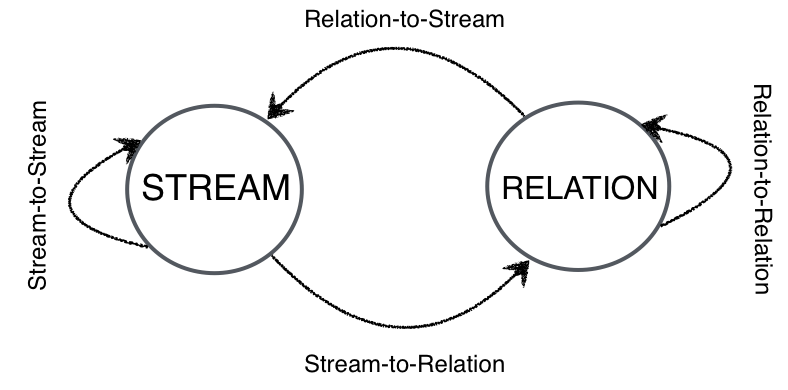
\includegraphics[width=0.7\textwidth]{relation}
\caption{FlinkCQL operators}
\label{fig:relation}
\end{figure}


%\subsection*{Denotation Language}
%\subsection*{Lamda Calculus}
%\subsection{Abstract Syntax}
%\subsection{Domain}
%\subsection{Denotation Semantics}


\subsection*{Stream-to-Stream}
\begin{enumerate}
	\item Projection
	
	$\mathcal{M}_{S2S}\sembrack{Select(A_1,A_2,..,A_k)} \\
		{}\qquad= \lambda_S.\{<(v.A_1,v.A_2,...,v.A_k),\tau_{app},\tau_{sys}>: \forall s<v,\tau_{app},\tau_{sys}>\in S \\
		{}\qquad\land (A_1,A_2,..,A_k) \subset Schema \}$ 
		
	\item Selection
	
	$\mathcal{M}_{S2S}\sembrack{Where(p)} \\
		{}\qquad= \lambda_S.\{s: \forall s \in S  \land p(s.v) = true \}$ 
		
	\item Merge/Union
	$\mathcal{M}_{S2S}\sembrack{Merge} \\
		{}\qquad= \lambda_{S_1}\lambda_{S_1}...\lambda_{S_k}.\{s: s \in S_1 \lor s \in S_1 \lor ... \lor s \in S_k \}$ 
	
	\item Split
	$\mathcal{M}_{S2S}\sembrack{Split} \\
		{}\qquad= \lambda_{S}.\lambda_{f}.\{s: s \in S \land f(s.v) = true \}$ 
	\item Grouping
	
	$\mathcal{M}_{S2S}\sembrack{GroupBy(A_1,A_2,..,A_k)} \\
		{}\qquad= \lambda_S.\lambda_{a_1}.\lambda_{a_2}...\lambda_{a_k}.\{s: s \in S  \land  s.v.A_i= a_i \,for\, \forall i \in [1,k]\\
		{}\qquad\land (A_1,A_2,..,A_k) \subset Schema \}$ 
\end{enumerate}

\subsection*{Stream-to-Relation}
\begin{enumerate}
	\item Application-time based
	$\mathcal{M}_{S2R}\sembrack{Size\, T\, on\, A} \\
		{}\qquad= \lambda_S.\lambda_{t_{app}}\{v:  s<v,t_{app}',t_{sys}> \in S  \land t'_{app} = v.A \\
		{}\qquad max(T-t_{app},0) < t'_{app} \leq t_{app} \}$ 
		
	\item System-time based
	
	$\mathcal{M}_{S2R}\sembrack{Size\, T\, milliseconds} \\
		{}\qquad= \lambda_S.\lambda_{t_{sys}}.\{v:  s<v,t_{app},t'_{sys}> \in S  \land 
		max(T-t_{sys},0) < t'_{sys} \leq t_{sys} \}$ 
		
	\item Count-based
	
	$\mathcal{M}_{S2R}\sembrack{Size\, N} \\
		{}\qquad= \lambda_S.\lambda_{t_{sys}}\{v:  s<v,t_{app},t'_{sys}> \in S  \land (t'_{sys} \leq t_{sys}) \\
		{}\qquad \land (N \geqslant |\{<e'',t''_{app},t''_{sys}> \in S: t'_{sys} \leq t''_{sys} \leq t_{sys}\}|) \}$
\end{enumerate}

\subsection*{Relation-to-Relation}
\begin{enumerate}
		
	\item Production
	
	$\mathcal{M}_{R2R}\sembrack{CrossJoin} \\
		{}\qquad= \lambda_{t_{sys}}.\lambda_{t_{sys}}.\{(e_1,e_2) : e_1 \in E_1 \land e_2 \in E_2 \}$
		
	\item Join
	
	$\mathcal{M}_{R2R}\sembrack{InnerJoin(a,b)} \\
		{}\qquad= \lambda_{E_1}.\lambda_{E_2}.\{(e_1,e_2) : e_1 \in E_1 \land e_2 \in E_2 \land e_1.a = e_2.b \land a \in Schema(e_1) \\
		{}\qquad= \land b \in Schema(e_2) \}$
		
	\item Grouping
	
		$\mathcal{M}_{R2R}\sembrack{GroupBy(A_1,A_2,..,A_k) Selection(AggFunc)} \\
		{}\qquad= \lambda_E.\lambda_{a_1}.\lambda_{a_2}...\lambda_{a_k}.\{AggFunc(E)  \land  \forall e \in E, \,\forall i \in [1,k] e.A_i= a_i \, \\
		{}\qquad\land (A_1,A_2,..,A_k) \subset Schema(e) \}$ 
	
	\item Projection
	
		$\mathcal{M}_{R2R}\sembrack{Select(A_1,A_2,..,A_k)} \\
		{}\qquad= \lambda_E.\{(e.A_1,e.A_2,...,e.A_k):e \in E \\
		{}\qquad\land (A_1,A_2,..,A_k) \subset Schema(e) \}$
	
\end{enumerate}

%\subsection*{Relation-to-Stream}
%$\mathcal{M}_{R2S}\sembrack{IStream} \\
%		{}\qquad= \lambda_R.\lambda_{t_{sys}}.\{v:  s<v,t_{app},t'_{sys}> \in S  \land 
%		max(T-t_{sys},0) < t'_{sys} \leq t_{sys} \}$ 

// TODO: Zoltan: some conclusion, reflection

%*******************************************************************************
%****************************** Second Chapter *********************************
%*******************************************************************************

\chapter{Implementations}

\ifpdf
    \graphicspath{{Chapter5/Figs/Raster/}{Chapter5/Figs/PDF/}{Chapter5/Figs/}}
\else
    \graphicspath{{Chapter5/Figs/Vector/}{Chapter5/Figs/}}
\fi

\section{Architecture}

\begin{figure}[h!] 
\centering    
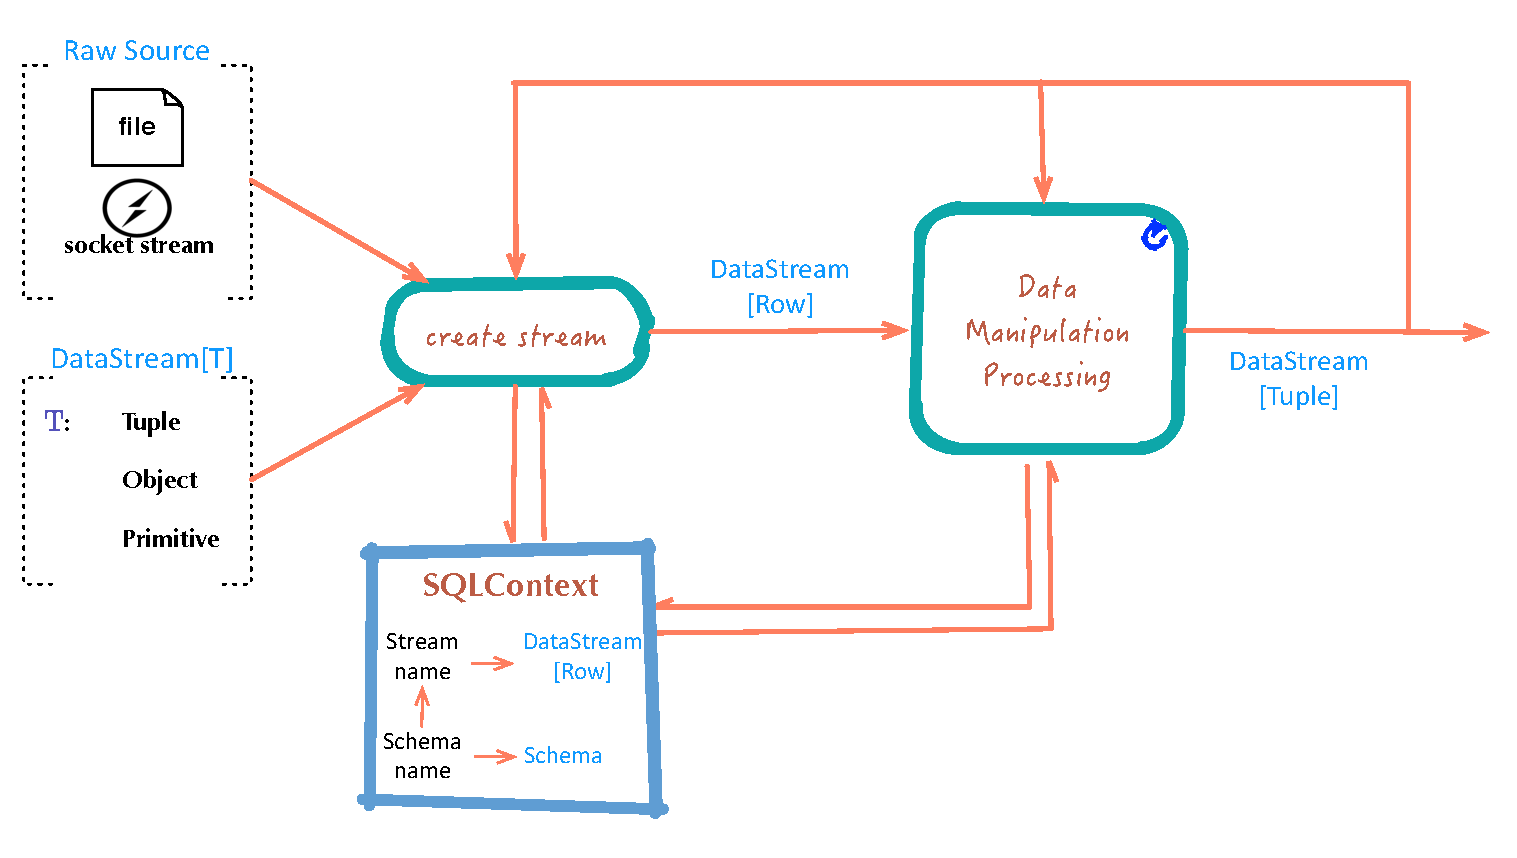
\includegraphics[width=1\textwidth]{Architecture}
\caption{Architecture}
\label{fig:Architecture}
\end{figure}


Figure~\ref{fig:Architecture} depicts the overall architecture of FlinkCQL query processing layer. It accepts data streams, query string and SQLContext as inputs and return one or more output data streams.
\subsection{Input Sources}
The query processing layer can connect to and process data streams from different data sources like file sources, web sockets, message queues (Apache Kafka, RabbitMQ, Twitter Streaming API …), and also from any user defined data sources. We classify the sources into 2 categories: \textit{Raw source} and predefined \textit{DataStream[T]} with \textit{T} is the type of elements.

\subsubsection*{Raw Source}


\textbf{Text file stream}: the source stream contains the lines of the files created (or modified) in a given directory. The system continuously monitors the given path, and processes any new files or modifications. The file will be read with the system’s default character set. FlinkCQL expresses the text file stream source via ``SOURCE FILE ( \textit{filePath, delimiter})'', the default delimiter is a comma. The delimiter is used to tokenize string and convert its result into tuples according to a schema


\textbf{Socket text stream}: the source stream contains the strings received from the given socket. Strings are decoded by the system’s default character set. Socket text stream is specified in FlinkCQL as ``SOURCE SOCKET ( \textit{filePath, delimiter})''
The user can optionally set a delimiter for the same purpose as in Text file stream.


\textbf{Message queue connectors:} There are pre-implemented connectors for a number of popular message queue services. Connectors provide an interface for accessing data from various third party sources (message queues). Currently three connectors are natively supported, namely Apache Kafka, RabbitMQ and the Twitter Streaming API. In the recent prototype of FlinkCQL, we have not designed any syntax for those connectors due to lacking of testing facilities. However, in the next prototype, we could extend its syntax at ease.

\subsection*{DataStream[T]}
The \textit{DataStream[T]} is the basic data abstraction provided by Flink Streaming. It represents a continuous, parallel, immutable stream of data of a certain type \textit{T}. Type \textit{T} could be :
\begin{itemize}
\item Primitive data type: integer, double, ...
\item Tuple type: which is a composite of multiple primitive data types such as \textit{(integer, string, integer)}
\item Class object: such as \textit{CarEvent(id: Int, speed: Int)}
\end{itemize} 

\subsection{SQL Context} 

At the beginning, we encounter a problem of diverse data types of stream elements. A source stream can contains elements of string type (as in raw source), other primitive types, tuple or class instance. It is cumbersome and impractical to provide query processing for all kinds of source streams respectively. Thus, when a data stream is entitled to a schema (via \textit{Create Stream} or \textit{Insert} statement), we first transform the origin source stream to a Data Stream of a universal type \textit{Row} . \textit{Row} is simply a tuple containing \textit{an array of any data} including \textit{Null}. We do not specify the type of elements inside the Row. Those types will be derived from Schema.

Recall the example in ~\ref{query:createStream} to create schema and stream of ``StockTick''.
\begin{lstlisting}
	CREATE SCHEMA StockTickSchema (symbol String, sourceTimestamp Long, price Double, quantity Int, exchange String)
\end{lstlisting}

\begin{lstlisting} 
	CREATE STREAM StockTick StockTickSchema 
	SOURCE SOCKET ("98.138.253.109", 2000)
\end{lstlisting}

``StockTick'' is the Stream used inside FlinkCQL query. It is entitled to ``StockTickSchema'' and mapped to a real \textit{DataStream[Row]} which is derived from the socket text stream. The correlation between Stream and Schema is expressed in Figure~\ref{fig:SQLContext}. Be aware that the concept of Stream in FlinkSQL and DataStream in Flink is not identical. In fact, a Stream in FlinkSQL is a name to represent a \textit{DataStream[T]} in Flink.

All Stream-Schema-DataStream relationships are stored in 3 dictionaries of \textit{SQLContext}~(Figure~\ref{fig:Architecture}). 
Stream and Schema are unique but many Stream can share a Schema. And a Stream is mapped to a DataStream[T]. When user send out some further queries, query processing framework will lookup \textit{SQLContext} to decide which Stream-Schema is specified to generate an precise snippet of code.

\begin{figure}[h!] 
\centering    
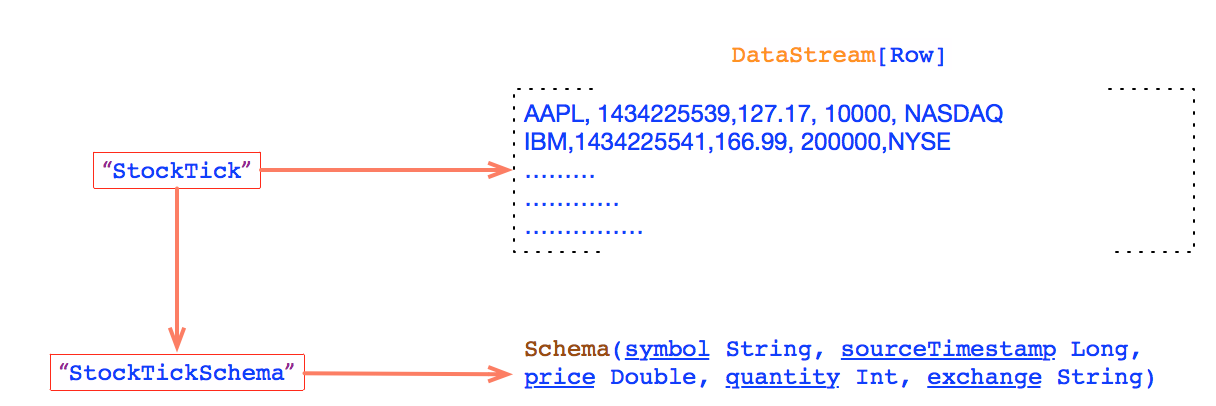
\includegraphics[width=0.8\textwidth]{SQLContext}
\caption{\textit{Stream}-\textit{Schema} mapping in \textit{SQLContext}}
\label{fig:SQLContext}
\end{figure}

\subsection{Data Manipulation Processing}
Data Manipulation Processing is used to process Data Manipulation Queries such as SELECT, MERGE, SPLIT, INSERT. These queries specify which operators to process on given Streams and its Fields. System will look up its SQLContext to retrieve the actual input DataStream[Row]. Operator and Schema are to decide how to transform input DataStreams to a new one. The output of processing is either one or more Streams which are updated into SQLContext or a DataStream of tuple. This DataStream of tuple can be consumed to create other Stream via \textit{CREATE STREAM} query. For examples, the output of \textit{SELECT} query is a DataStream of tuple but the outputs of \textit{SPLIT} query are more than one Stream~(along with its Schema and DataStream[Row]).

\section{FlinkCQL Query Interpreter}
\begin{figure}[h!] 
\centering    
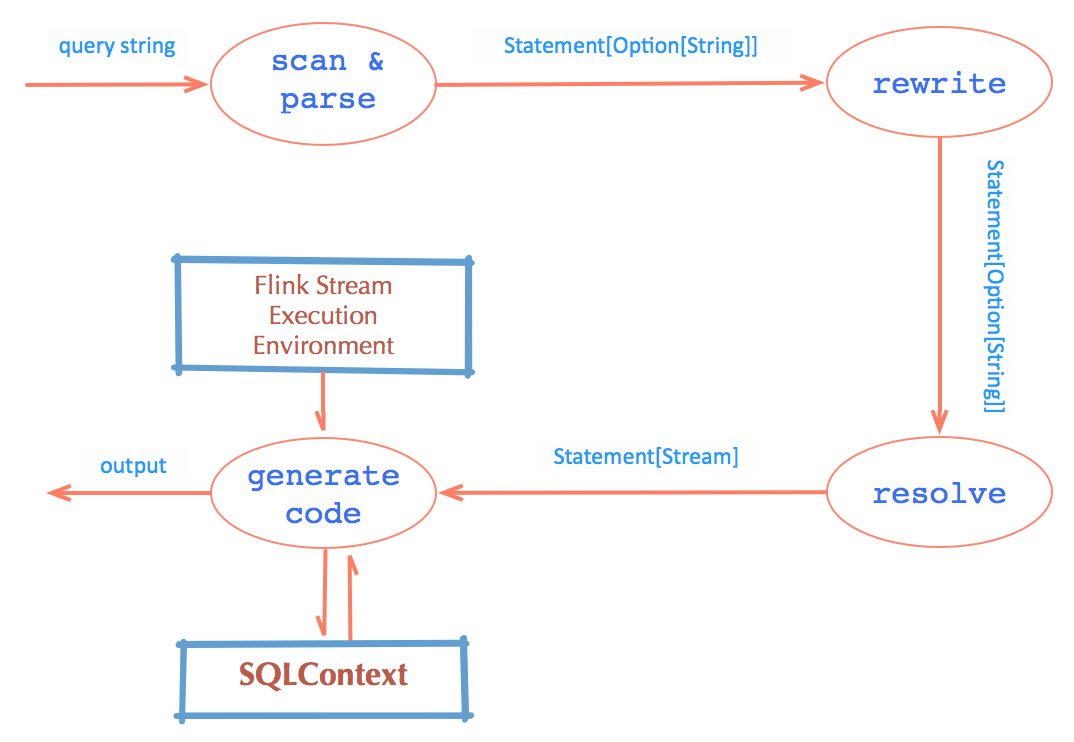
\includegraphics[width=0.7\textwidth]{QueryProcessing}
\caption{Query Processing}
\label{fig:QueryProcessing}
\end{figure}


//TODO: Tree-Based Interpreter~\citep{Parr:2009}
[Programming Language Pragmatics, Third Edition.pdf page 57


Flink Stream Processing is offering a rich set of API to deal with one or  multiple input DataStream[T]. Our goal is to build an extension which accepts FlinkCQL query strings as commands and translate the commands to  corresponding programs constructed with Flink's APIs. Thus we are simply required to build a interpreter instead of a compiler from a scratch. For the purpose, I have implemented a tree-based interpreter~\citep{Parr:2009} to process FlinkCQL query. The idea is that the query interpreter executes program by constructing an abstract syntax tree~(AST) from the input query string and walking through the tree to generate a executable Flink program. More specifically, AST is a form of intermediate representation of the hierarchical syntactical structure of the source program written in query.  
	

The interpretation proceed through a series of well-defined phrases (Figure~\ref{fig:QueryProcessing}). Each phrase transforms or extracts information of use from the output of previous phrase and return a result which is a input of next phrase. In first proof-of-concept prototype, we build a pipeline consisting of 4 steps:
\begin{itemize}
	\item \textbf{Scanning and parsing:} serve to recognize the structure of the program, without regard to its meaning. This steps produce an AST with its root is highest semantic level of query : \textit{Statement[Option[String]]}

	\item \textbf{Rewriting} is to modify a sub-tree of AST to a more compact, optimal AST without changing the semantic of program.
	
	\item \textbf{Resolving:} It is possible that two or more streams, which are specified in query,  shares the same Schema. Thus, there is a potential ambiguity between two fields which have a identical name but belong to different stream. This phrase is to figure out to which fields refers. It is clear that we cannot generate code from an ambiguous AST.
	
	\item \textbf{Code generation}: In addition to a compact and unambiguous AST, the interpreter also lookup Stream-Schema information from SQLContext to generate a Flink program based on pre-defined translation rules. Last but not at least, we need the Flink stream execution environment to execute our generated code.
	
I describe all phrases in following: 
	
\end{itemize}
\subsection{Scanning and Parsing}


 Heterogeneous AST

[Manning.DSLs.in.Action.pdf
Packrat parsing for left recursive DSL syntax

A DSL that needs a packrat parser


\begin{itemize}
	\item Step 1: Executing the grammar
	\item Step 2: Building the semantic model for the DSL
	\item Step 3: Designing the Order abstraction
	\item Step 4: Generating the AST using function application combinators
\end{itemize}




\begin{figure}[h!] 
\centering    
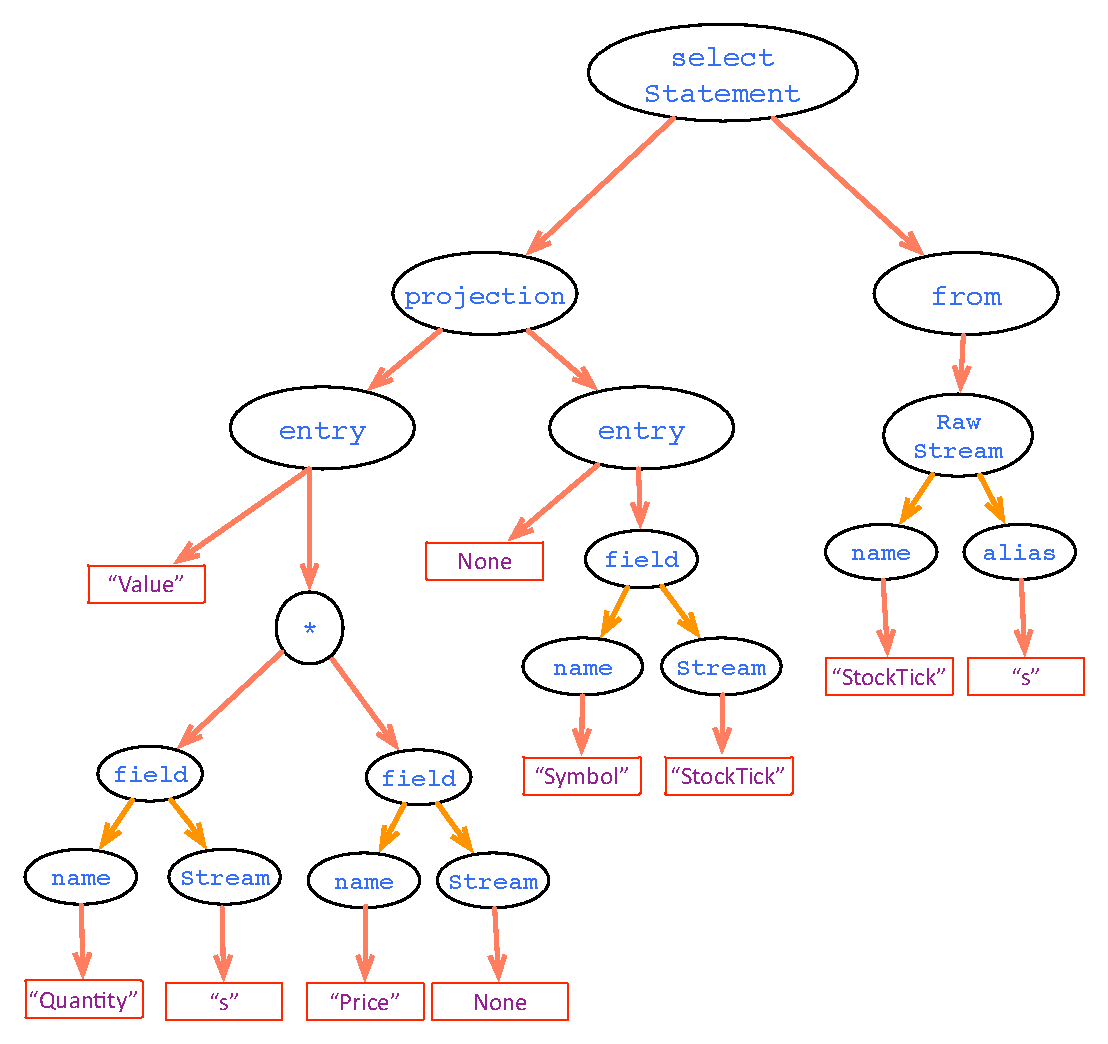
\includegraphics[width=0.7\textwidth]{Parse}
\caption{Parse}
\label{fig:Parse}
\end{figure}


\subsection{Query Rewriting}
Pattern Matching

We apply one rewriting rule for subquery:
\begin{lstlisting}
From (select Symbol,Price From StockTick [Size 3]) as s
=
From (select Symbol,Price From StockTick) [Size 3] as s
\end{lstlisting}

In the first query , its subquery will return a Windowed Stream which is not supported now. Therefore the query is invalid

In the second query, its subquery return a concrete DataStream which is acceptable.

However, the 2 queries are identical in term of semantics. Thus, we transform the first to the second.


\subsection{Resolving}
\begin{figure}[h!] 
\centering    
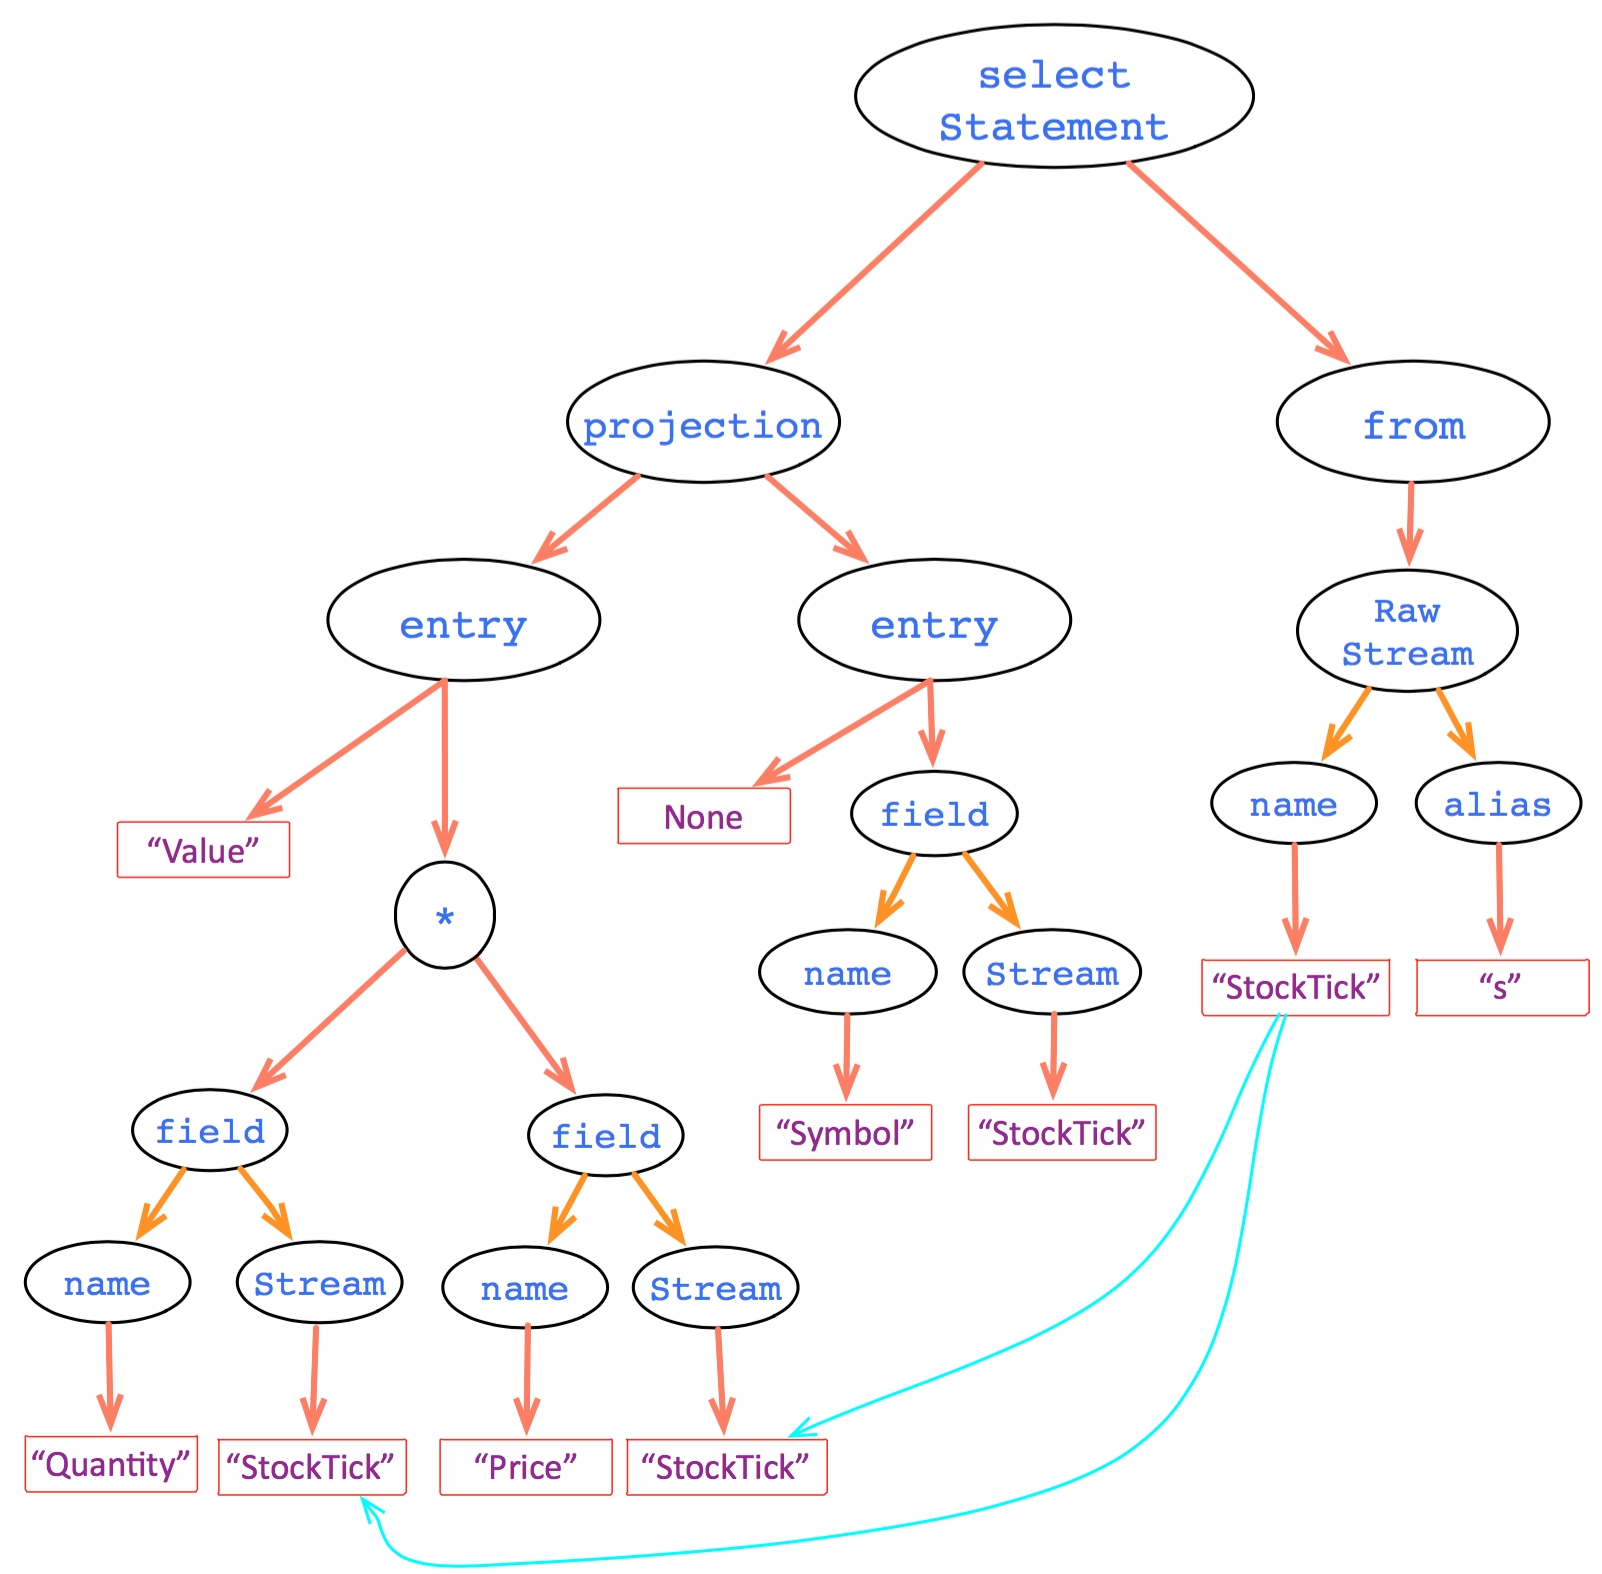
\includegraphics[width=0.7\textwidth]{Resolve}
\caption{Resolve}
\label{fig:Resolve}
\end{figure}

Pattern Matching
15 Tree pattern matcher


In the example, we are going to figure out  which streams that “StockTick.Symbol”, “s.Quantity”, “Price”  projections refer to. This step is important because perhaps many different streams have 2 fields which have an identical name. For example, 2 streams may own a field which is “Price”. 
This step helps to resolve which fields belongs to which streams so that we can generate the exact code for the query


\subsection{Code Generation}
Using Scala compile-time and run-time reflection to build a Scala Abstract Syntax Tree


Translation Rule


\section{Evaluations}

Compare to other systems


\section{Future Works}

Dynamic variable


http://www.sqlstream.com/blog/2015/03/5-reasons-why-spark-streamings-batch-processing-of-data-streams-is-not-stream-processing/



Data Input
http://flink.apache.org/news/2015/05/11/Juggling-with-Bits-and-Bytes.html


http://ci.apache.org/projects/flink/flink-docs-master/internals/fig/stack.svg

http://ci.apache.org/projects/flink/flink-docs-master/internals/general\_arch.html

%%*******************************************************************************
% * <duyvk142@gmail.com> 2015-04-13T09:15:03.064Z:
%
% 
%
%*********************************** First Chapter *****************************
%*******************************************************************************
% ^ <duyvk142@gmail.com> 2015-04-13T09:18:08.942Z.

\chapter{Getting started}  %Title of the First Chapter

\ifpdf
    \graphicspath{{Chapter01/Figs/Raster/}{Chapter01/Figs/PDF/}{Chapter01/Figs/}}
\else
    \graphicspath{{Chapter01/Figs/Vector/}{Chapter01/Figs/}}
\fi


%********************************** %First Section  **************************************
\section{What is loren ipsum? Title with math \texorpdfstring{$\sigma$}{[sigma]}} %Section - 1.1 

\begin{defi}
This is a definition
\end{defi}


\begin{defi}
This is a definition
\end{defi}

Lorem Ipsum is simply dummy text of the printing and typesetting industry (see 
Section~\ref{section1.3}). Lorem Ipsum~\citep{Aup91} has been the industry's 
standard dummy text ever since the 1500s, when an unknown printer took a galley 
of type and scrambled it to make a type specimen book. It has survived not only 
five centuries, but also the leap into electronic typesetting, remaining 
essentially unchanged. It was popularised in the 1960s with the release of 
Letraset sheets containing Lorem Ipsum passages, and more recently with desktop 
publishing software like Aldus PageMaker including versions of Lorem 
Ipsum~\citep{AAB95,Con90,LM65}.

The most famous equation in the world: $E^2 = (m_0c^2)^2 + (pc)^2$, which is 
known as the \textbf{energy-mass-momentum} relation as an in-line equation.

A {\em \LaTeX{} class file}\index{\LaTeX{} class file@LaTeX class file} is a file, which holds style information for a particular \LaTeX{}.


%\begin{align}
%CIF: \hspace*{5mm}F_0^j(a) = \frac{1}{2\pi \iota} \oint_{\gamma} \frac{F_0^j(z)}{z - a} dz
%\end{align}


\begin{equation}
	y_t = a_1y_{t-1}+a_2y_{t-2}+...+a_py_{t-p}+\epsilon_t
\end{equation}

\nomenclature[z-cif]{$CIF$}{Cauchy's Integral Formula}                                % first letter Z is for Acronyms 
\nomenclature[a-F]{$F$}{complex function}                                                   % first letter A is for Roman symbols
\nomenclature[g-p]{$\pi$}{ $\simeq 3.14\ldots$}                                             % first letter G is for Greek Symbols
\nomenclature[g-i]{$\iota$}{unit imaginary number $\sqrt{-1}$}                      % first letter G is for Greek Symbols
\nomenclature[g-g]{$\gamma$}{a simply closed curve on a complex plane}  % first letter G is for Greek Symbols
\nomenclature[x-i]{$\oint_\gamma$}{integration around a curve $\gamma$} % first letter X is for Other Symbols
\nomenclature[r-j]{$j$}{superscript index}                                                       % first letter R is for superscripts
\nomenclature[s-0]{$0$}{subscript index}                                                        % first letter S is for subscripts


%********************************** %Second Section  *************************************
\section{Why do we use loren ipsum?} %Section - 1.2


It is a long established fact that a reader will be distracted by the readable content of a page when looking at its layout. The point of using Lorem Ipsum is that it has a more-or-less normal distribution of letters, as opposed to using `Content here, content here', making it look like readable English. Many desktop publishing packages and web page editors now use Lorem Ipsum as their default model text, and a search for `lorem ipsum' will uncover many web sites still in their infancy. Various versions have evolved over the years, sometimes by accident, sometimes on purpose (injected humour and the like).

%********************************** % Third Section  *************************************
\section{Where does it come from?}  %Section - 1.3 
\label{section1.3}

Contrary to popular belief, Lorem Ipsum is not simply random text. It has roots in a piece of classical Latin literature from 45 BC, making it over 2000 years old. Richard McClintock, a Latin professor at Hampden-Sydney College in Virginia, looked up one of the more obscure Latin words, consectetur, from a Lorem Ipsum passage, and going through the cites of the word in classical literature, discovered the undoubtable source. Lorem Ipsum comes from sections 1.10.32 and 1.10.33 of "de Finibus Bonorum et Malorum" (The Extremes of Good and Evil) by Cicero, written in 45 BC. This book is a treatise on the theory of ethics, very popular during the Renaissance. The first line of Lorem Ipsum, "Lorem ipsum dolor sit amet..", comes from a line in section 1.10.32.

The standard chunk of Lorem Ipsum used since the 1500s is reproduced below for those interested. Sections 1.10.32 and 1.10.33 from ``de Finibus Bonorum et Malorum" by Cicero are also reproduced in their exact original form, accompanied by English versions from the 1914 translation by H. Rackham

``Lorem ipsum dolor sit amet, consectetur adipisicing elit, sed do eiusmod tempor incididunt ut labore et dolore magna aliqua. Ut enim ad minim veniam, quis nostrud exercitation ullamco laboris nisi ut aliquip ex ea commodo consequat. Duis aute irure dolor in reprehenderit in voluptate velit esse cillum dolore eu fugiat nulla pariatur. Excepteur sint occaecat cupidatat non proident, sunt in culpa qui officia deserunt mollit anim id est laborum."

Section 1.10.32 of ``de Finibus Bonorum et Malorum", written by Cicero in 45 BC: ``Sed ut perspiciatis unde omnis iste natus error sit voluptatem accusantium doloremque laudantium, totam rem aperiam, eaque ipsa quae ab illo inventore veritatis et quasi architecto beatae vitae dicta sunt explicabo. Nemo enim ipsam voluptatem quia voluptas sit aspernatur aut odit aut fugit, sed quia consequuntur magni dolores eos qui ratione voluptatem sequi nesciunt. Neque porro quisquam est, qui dolorem ipsum quia dolor sit amet, consectetur, adipisci velit, sed quia non numquam eius modi tempora incidunt ut labore et dolore magnam aliquam quaerat voluptatem. Ut enim ad minima veniam, quis nostrum exercitationem ullam corporis suscipit laboriosam, nisi ut aliquid ex ea commodi consequatur? Quis autem vel eum iure reprehenderit qui in ea voluptate velit esse quam nihil molestiae consequatur, vel illum qui dolorem eum fugiat quo voluptas nulla pariatur?"

1914 translation by H. Rackham: ``But I must explain to you how all this mistaken idea of denouncing pleasure and praising pain was born and I will give you a complete account of the system, and expound the actual teachings of the great explorer of the truth, the master-builder of human happiness. No one rejects, dislikes, or avoids pleasure itself, because it is pleasure, but because those who do not know how to pursue pleasure rationally encounter consequences that are extremely painful. Nor again is there anyone who loves or pursues or desires to obtain pain of itself, because it is pain, but because occasionally circumstances occur in which toil and pain can procure him some great pleasure. To take a trivial example, which of us ever undertakes laborious physical exercise, except to obtain some advantage from it? But who has any right to find fault with a man who chooses to enjoy a pleasure that has no annoying consequences, or one who avoids a pain that produces no resultant pleasure?"

Section 1.10.33 of ``de Finibus Bonorum et Malorum", written by Cicero in 45 BC: ``At vero eos et accusamus et iusto odio dignissimos ducimus qui blanditiis praesentium voluptatum deleniti atque corrupti quos dolores et quas molestias excepturi sint occaecati cupiditate non provident, similique sunt in culpa qui officia deserunt mollitia animi, id est laborum et dolorum fuga. Et harum quidem rerum facilis est et expedita distinctio. Nam libero tempore, cum soluta nobis est eligendi optio cumque nihil impedit quo minus id quod maxime placeat facere possimus, omnis voluptas assumenda est, omnis dolor repellendus. Temporibus autem quibusdam et aut officiis debitis aut rerum necessitatibus saepe eveniet ut et voluptates repudiandae sint et molestiae non recusandae. Itaque earum rerum hic tenetur a sapiente delectus, ut aut reiciendis voluptatibus maiores alias consequatur aut perferendis doloribus asperiores repellat."

1914 translation by H. Rackham: ``On the other hand, we denounce with righteous indignation and dislike men who are so beguiled and demoralized by the charms of pleasure of the moment, so blinded by desire, that they cannot foresee the pain and trouble that are bound to ensue; and equal blame belongs to those who fail in their duty through weakness of will, which is the same as saying through shrinking from toil and pain. These cases are perfectly simple and easy to distinguish. In a free hour, when our power of choice is untrammelled and when nothing prevents our being able to do what we like best, every pleasure is to be welcomed and every pain avoided. But in certain circumstances and owing to the claims of duty or the obligations of business it will frequently occur that pleasures have to be repudiated and annoyances accepted. The wise man therefore always holds in these matters to this principle of selection: he rejects pleasures to secure other greater pleasures, or else he endures pains to avoid worse pains."

%%*******************************************************************************
%****************************** Second Chapter *********************************
%*******************************************************************************

\chapter{My second chapter}

\ifpdf
    \graphicspath{{Chapter02/Figs/Raster/}{Chapter02/Figs/PDF/}{Chapter02/Figs/}}
\else
    \graphicspath{{Chapter02/Figs/Vector/}{Chapter02/Figs/}}
\fi


\section[Short title]{Reasonably long section title}
\subsection{This is a short title}

% Uncomment this line, when you have siunitx package loaded.
%The SI Units for dynamic viscosity is \si{\newton\second\per\metre\squared}.

I'm going to randomly include a picture Figure~\ref{fig:minion}.


If you have trouble viewing this document contact Krishna at: \href{mailto:kks32@cam.ac.uk}{kks32@cam.ac.uk} or raise an issue at \url{https://github.com/kks32/phd-thesis-template/}


\begin{figure}[htbp!] 
\centering    

\includegraphics[width=1.0\textwidth]{minion}
\caption[Minion]{This is just a long figure caption for the minion in Despicable Me from Pixar}
\label{fig:minion}
\end{figure}


\section*{Enumeration}
\begin{enumerate}
\item The first topic is dull
\item The second topic is duller
\begin{enumerate}
\item The first subtopic is silly
\item The second subtopic is stupid
\end{enumerate}
\item The third topic is the dullest
\end{enumerate}

\section*{itemize}
\begin{itemize}
\item The first topic is dull
\item The second topic is duller
\begin{itemize}
\item The first subtopic is silly
\item The second subtopic is stupid
\end{itemize}
\item The third topic is the dullest
\end{itemize}

\section*{description}
\begin{description}
\item[The first topic] is dull
\item[The second topic] is duller
\begin{description}
\item[The first subtopic] is silly
\item[The second subtopic] is stupid
\end{description}
\item[The third topic] is the dullest
\end{description}


\clearpage

\tochide\section{Hidden section}
\textbf{Lorem ipsum dolor sit amet}, \textit{consectetur adipiscing elit}. In magna nisi, aliquam id blandit id, congue ac est. Fusce porta consequat leo. Proin feugiat at felis vel consectetur. Ut tempus ipsum sit amet congue posuere. Nulla varius rutrum quam. Donec sed purus luctus, faucibus velit id, ultrices sapien. Cras diam purus, tincidunt eget tristique ut, egestas quis nulla. Curabitur vel iaculis lectus. Nunc nulla urna, ultrices et eleifend in, accumsan ut erat. In ut ante leo. Aenean a lacinia nisl, sit amet ullamcorper dolor. Maecenas blandit, tortor ut scelerisque congue, velit diam volutpat metus, sed vestibulum eros justo ut nulla. Etiam nec ipsum non enim luctus porta in in massa. Cras arcu urna, malesuada ut tellus ut, pellentesque mollis risus.Morbi vel tortor imperdiet arcu auctor mattis sit amet eu nisi. Nulla gravida urna vel nisl egestas varius. Aliquam posuere ante quis malesuada dignissim. Mauris ultrices tristique eros, a dignissim nisl iaculis nec. Praesent dapibus tincidunt mauris nec tempor. Curabitur et consequat nisi. Quisque viverra egestas risus, ut sodales enim blandit at. Mauris quis odio nulla. Cras euismod turpis magna, in facilisis diam congue non. Mauris faucibus nisl a orci dictum, et tempus mi cursus.

Etiam elementum tristique lacus, sit amet eleifend nibh eleifend sed \footnote{My footnote goes blah blah blah! \dots}. Maecenas dapibu augue ut urna malesuada, non tempor nibh mollis. Donec sed sem sollicitudin, convallis velit aliquam, tincidunt diam. In eu venenatis lorem. Aliquam non augue porttitor tellus faucibus porta et nec ante. Proin sodales, libero vitae commodo sodales, dolor nisi cursus magna, non tincidunt ipsum nibh eget purus. Nam rutrum tincidunt arcu, tincidunt vulputate mi sagittis id. Proin et nisi nec orci tincidunt auctor et porta elit. Praesent eu dolor ac magna cursus euismod. Integer non dictum nunc.
\ref{fig:Minnion}


\begin{landscape}

\section*{Subplots}
I can cite Wall-E (see Fig.~\ref{fig:WallE}) and Minions in despicable me (Fig.~\ref{fig:Minnion}) or I can cite the whole figure as Fig.~\ref{fig:animations}


\begin{figure}
  \centering
  \begin{subfigure}[b]{0.3\textwidth}
    
\includegraphics[width=\textwidth]{TomandJerry}
    \caption{Tom and Jerry}
    \label{fig:TomJerry}   
  \end{subfigure}             
  \begin{subfigure}[b]{0.3\textwidth}
    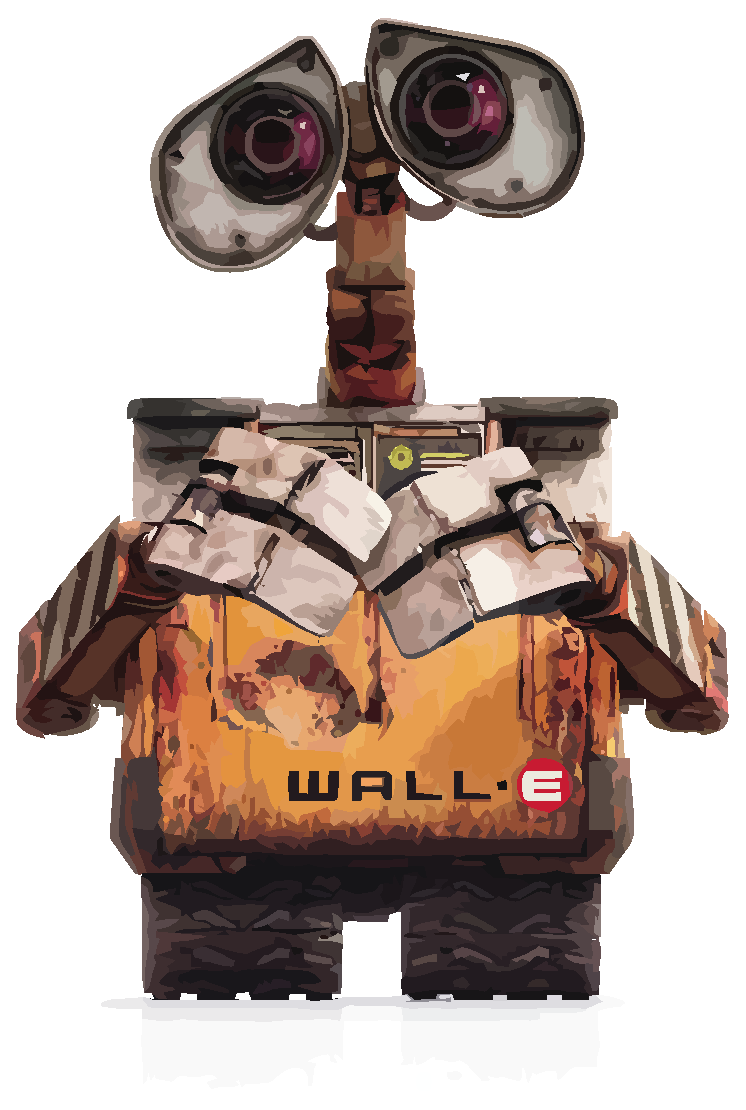
\includegraphics[width=\textwidth]{WallE}
    \caption{Wall-E}
    \label{fig:WallE}
  \end{subfigure}             
  \begin{subfigure}[b]{0.3\textwidth}
    
\includegraphics[width=\textwidth]{minion}
    \caption{Minions}
    \label{fig:Minnion}
  \end{subfigure}
  \caption{Best Animations}
  \label{fig:animations}
\end{figure}


\end{landscape}

%\chapter{My third chapter}

% **************************** Define Graphics Path **************************
\ifpdf
    \graphicspath{{Chapter3/Figs/Raster/}{Chapter3/Figs/PDF/}{Chapter3/Figs/}}
\else
    \graphicspath{{Chapter3/Figs/Vector/}{Chapter3/Figs/}}
\fi

\section{First section of the third chapter}
And now I begin my third chapter here \dots

And now to cite some more people~\citet{Rea85,Ancey1996}

\subsection{First subsection in the first section}
\dots and some more 

\subsection{Second subsection in the first section}
\dots and some more \dots

\subsubsection{First subsub section in the second subsection}
\dots and some more in the first subsub section otherwise it all looks the same
doesn't it? well we can add some text to it \dots

\subsection{Third subsection in the first section}
\dots and some more \dots

\subsubsection{First subsub section in the third subsection}
\dots and some more in the first subsub section otherwise it all looks the same
doesn't it? well we can add some text to it and some more and some more and
some more and some more and some more and some more and some more \dots

\subsubsection{Second subsub section in the third subsection}
\dots and some more in the first subsub section otherwise it all looks the same
doesn't it? well we can add some text to it \dots

\section{Second section of the third chapter}
and here I write more \dots

\section{The layout of formal tables}
This section has been modified from ``Publication quality tables in \LaTeX*''
 by Simon Fear.

The layout of a table has been established over centuries of experience and 
should only be altered in extraordinary circumstances. 

When formatting a table, remember two simple guidelines at all times:

\begin{enumerate}
  \item Never, ever use vertical rules (lines).
  \item Never use double rules.
\end{enumerate}

These guidelines may seem extreme but I have
never found a good argument in favour of breaking them. For
example, if you feel that the information in the left half of
a table is so different from that on the right that it needs
to be separated by a vertical line, then you should use two
tables instead. Not everyone follows the second guideline:

There are three further guidelines worth mentioning here as they
are generally not known outside the circle of professional
typesetters and subeditors:

\begin{enumerate}\setcounter{enumi}{2}
  \item Put the units in the column heading (not in the body of
          the table).
  \item Always precede a decimal point by a digit; thus 0.1
      {\em not} just .1.
  \item Do not use `ditto' signs or any other such convention to
      repeat a previous value. In many circumstances a blank
      will serve just as well. If it won't, then repeat the value.
\end{enumerate}

A frequently seen mistake is to use `\textbackslash begin\{center\}' \dots `\textbackslash end\{center\}' inside a figure or table environment. This center environment can cause additional vertical space. If you want to avoid that just use `\textbackslash centering'


\begin{table}
\caption{A badly formatted table}
\centering
\label{table:bad_table}
\begin{tabular}{|l|c|c|c|c|}
\hline 
& \multicolumn{2}{c}{Species I} & \multicolumn{2}{c|}{Species II} \\ 
\hline
Dental measurement  & mean & SD  & mean & SD  \\ \hline 
\hline
I1MD & 6.23 & 0.91 & 5.2  & 0.7  \\
\hline 
I1LL & 7.48 & 0.56 & 8.7  & 0.71 \\
\hline 
I2MD & 3.99 & 0.63 & 4.22 & 0.54 \\
\hline 
I2LL & 6.81 & 0.02 & 6.66 & 0.01 \\
\hline 
CMD & 13.47 & 0.09 & 10.55 & 0.05 \\
\hline 
CBL & 11.88 & 0.05 & 13.11 & 0.04\\ 
\hline 
\end{tabular}
\end{table}

\begin{table}
\caption{A nice looking table}
\centering
\label{table:nice_table}
\begin{tabular}{l c c c c}
\hline 
\multirow{2}{*}{Dental measurement} & \multicolumn{2}{c}{Species I} & \multicolumn{2}{c}{Species II} \\ 
\cline{2-5}
  & mean & SD  & mean & SD  \\ 
\hline
I1MD & 6.23 & 0.91 & 5.2  & 0.7  \\

I1LL & 7.48 & 0.56 & 8.7  & 0.71 \\

I2MD & 3.99 & 0.63 & 4.22 & 0.54 \\

I2LL & 6.81 & 0.02 & 6.66 & 0.01 \\

CMD & 13.47 & 0.09 & 10.55 & 0.05 \\

CBL & 11.88 & 0.05 & 13.11 & 0.04\\ 
\hline 
\end{tabular}
\end{table}


\begin{table}
\caption{Even better looking table using booktabs}
\centering
\label{table:good_table}
\begin{tabular}{l c c c c}
\toprule
\multirow{2}{*}{Dental measurement} & \multicolumn{2}{c}{Species I} & \multicolumn{2}{c}{Species II} \\ 
\cmidrule{2-5}
  & mean & SD  & mean & SD  \\ 
\midrule
I1MD & 6.23 & 0.91 & 5.2  & 0.7  \\

I1LL & 7.48 & 0.56 & 8.7  & 0.71 \\

I2MD & 3.99 & 0.63 & 4.22 & 0.54 \\

I2LL & 6.81 & 0.02 & 6.66 & 0.01 \\

CMD & 13.47 & 0.09 & 10.55 & 0.05 \\

CBL & 11.88 & 0.05 & 13.11 & 0.04\\ 
\bottomrule
\end{tabular}
\end{table}




% ********************************** Back Matter *******************************
% Backmatter should be commented out, if you are using appendices after References
%\backmatter

% ********************************** Bibliography ******************************
\begin{spacing}{0.9}

% To use the conventional natbib style referencing
% Bibliography style previews: http://nodonn.tipido.net/bibstyle.php
% Reference styles: http://sites.stat.psu.edu/~surajit/present/bib.htm

\bibliographystyle{apalike}
%\bibliographystyle{plainnat} % use this to have URLs listed in References
\cleardoublepage
\bibliography{References/references} % Path to your References.bib file


% If you would like to use BibLaTeX for your references, pass `custombib' as
% an option in the document class. The location of 'reference.bib' should be
% specified in the preamble.tex file in the custombib section.
% Comment out the lines related to natbib above and uncomment the following line.

%\printbibliography[heading=bibintoc, title={References}]


\end{spacing}

% ********************************** Appendices ********************************

\begin{appendices} % Using appendices environment for more functunality
%% ******************************* Thesis Appendix A ****************************
\chapter{Notices} 


\textbf{NOTE}
file:///Volumes/Data/WORKSPACE/git/thesis/rrd-antlr4/target/output/Json/index.html








\subsubsection*{Installation}
\begin{enumerate}
\item	Mount the ISO file in the mnt directory
\begin{verbatim}
mount -t iso9660 -o ro,loop,noauto /your/texlive####.iso /mnt
\end{verbatim}

\item	Install wget on your OS (use rpm, apt-get or yum install)
\item	Run the installer script install-tl.
\begin{verbatim}
	cd /your/download/directory
	./install-tl
\end{verbatim}
\item	Enter command `i' for installation

\item	Post-Installation configuration:\\
\href{http://www.tug.org/texlive/doc/texlive-en/texlive-en.html\#x1-320003.4.1}
{http://www.tug.org/texlive/doc/texlive-en/texlive-en.html\#x1-320003.4.1} 
\item	Set the path for the directory of TexLive binaries in your .bashrc file
\end{enumerate}

\subsubsection*{For 32bit OS}
For Bourne-compatible shells such as bash, and using Intel x86 GNU/Linux and a default directory setup as an example, the file to edit might be \begin{verbatim}
edit $~/.bashrc file and add following lines
PATH=/usr/local/texlive/2011/bin/i386-linux:$PATH; 
export PATH 
MANPATH=/usr/local/texlive/2011/texmf/doc/man:$MANPATH;
export MANPATH 
INFOPATH=/usr/local/texlive/2011/texmf/doc/info:$INFOPATH;
export INFOPATH
\end{verbatim}
\subsubsection*{For 64bit OS}
\begin{verbatim}
edit $~/.bashrc file and add following lines
PATH=/usr/local/texlive/2011/bin/x86_64-linux:$PATH;
export PATH 
MANPATH=/usr/local/texlive/2011/texmf/doc/man:$MANPATH;
export MANPATH 
INFOPATH=/usr/local/texlive/2011/texmf/doc/info:$INFOPATH;
export INFOPATH

\end{verbatim}



%% ******************************* Thesis Appendix B ********************************

\chapter{Installing the CUED class file}

\LaTeX.cls files can be accessed system-wide when they are placed in the
<texmf>/tex/latex directory, where <texmf> is the root directory of the user’s \TeX installation. On systems that have a local texmf tree (<texmflocal>), which
may be named ``texmf-local'' or ``localtexmf'', it may be advisable to install packages in <texmflocal>, rather than <texmf> as the contents of the former, unlike that of the latter, are preserved after the \LaTeX system is reinstalled and/or upgraded.

It is recommended that the user create a subdirectory <texmf>/tex/latex/CUED for all CUED related \LaTeX class and package files. On some \LaTeX systems, the directory look-up tables will need to be refreshed after making additions or deletions to the system files. For \TeX Live systems this is accomplished via executing ``texhash'' as root. MIK\TeX users can run ``initexmf -u'' to accomplish the same thing.

Users not willing or able to install the files system-wide can install them in their personal directories, but will then have to provide the path (full or relative) in addition to the filename when referring to them in \LaTeX.

\end{appendices}

% *************************************** Index ********************************
\printthesisindex % If index is present

\end{document}
